\documentclass[12pt]{report}
\usepackage{WSU}

%-----------------------------------------------------------------------
% Latex Thesis Template for Wright State University
% Written by Sean A. Mortara
% 28 June 2001
%-----------------------------------------------------------------------
%
%  Modified fields
%-----------------------------------------------------------------------
\newcommand{\authorfirst}{Orville}
\newcommand{\authorMI}{R.~}
\newcommand{\authorlast}{Bennett}
\newcommand{\degreefull}{Master of Science}
\newcommand{\degreeshort}{M.S.}
\newcommand{\dept}{Department of Neuroscience, Cell Biology and Physiology}
\newcommand{\institution}{Wright State University}
\newcommand{\thesistitle}{Expressing human Orai3 in insect cells for pharmacological studies}  % 
%No spaces should be before or after this title.
\newcommand{\pdfsubject}{     Store Operated Calcium Entry                }
\newcommand{\pdfkeywords}{    SOCE, Ca2+ entry, Calcium entry        }
\newcommand{\yearcomplete}{   2012}
%-----------------------------------------------------------------------
%  Thesis Advisor, Department Chair, Dean of Graduate Studies
%-----------------------------------------------------------------------
\newcommand{\thesisdirector}{J. Ashot Kozak}
\newcommand{\thesisdirectortitle}{Ph.D.}
\newcommand{\deptchair}{Timothy Cope}
\newcommand{\deptchairtitle}{Ph.D.}
\newcommand{\dean}{Andrew Hsu}
\newcommand{\deantitle}{Ph.D.}
%-----------------------------------------------------------------------
%  Final Examination Committee
%-----------------------------------------------------------------------
\newcommand{\fecone}{                    J. Ashot Kozak, Ph. D.            }

\newcommand{\fectwo}{                  Thomas Brown, Ph. D.            }

\newcommand{\fecthree}{                    Adrian Corbett, Ph. D.           }

%Uncomment for fourth committee member as needed. Also uncomment in WSU.sty file. 
\newcommand{\fecfour}{                  Robert Putnam, Ph. D.             }

% For more then 4 committee members, edit WSU.sty to insert fifth or so on. Sorry.


% Modify this if needed for getting citations to "look right" according to your field. Read the natbib documentation on how to use this. 
\usepackage{natbib}
%\usepackage[numbers,super]{natbib}
%\usepackage{utf8} % for utf-8 input
\usepackage{amsmath} % nice math symbols
%\usepackage{amssymb} % more math symbols
\usepackage{bm} % bold math
%\usepackage[usenames,dvipsnames]{color} % change text color
\usepackage[table,usenames,dvipsnames]{xcolor} % for adding color to table rows
\usepackage{multirow} % provides multiple row spanning table entries 
\usepackage{tikz}
\usepackage[colorinlistoftodos,textwidth=3cm]{todonotes} % for easy TODO creation
\reversemarginpar % use left margin
\setlength{\marginparwidth}{3cm} % use for todonotes margins
\usepackage{syntonly} % syntonly package: checks syntax only when next line is uncommented
%\syntaxonly
%\usepackage{epstopdf} % to convert EPS images to PDFs for use as figures
\usepackage{graphicx}
\DeclareGraphicsExtensions{.pdf,.eps,.jpg}

\usepackage[labelfont=bf]{caption} % Bold caption label

\usepackage{lpic}
\usetikzlibrary{decorations.pathmorphing} % for snake lines
\usetikzlibrary{matrix} % for block alignment
\usetikzlibrary{arrows} % for arrow heads
\usetikzlibrary{calc} % for manipulation of coordinates

\usepackage{paralist} % for in-paragraph lists
\usepackage{textcomp} % use for \textcelsius{}
\usepackage{subfig} 	% gives the author the ability to have subfigures within figures, or subtables within table floats.

%\usepackage{doublespace}
%\usepackage{setspace} % for control of spacing

% LaTeX macros specific to this thesis.
\newcommand\Ca{Ca$^{2+}$}
\newcommand\Mg{Mg$^{2+}$}
\newcommand\Na{Na$^{+}$}
\newcommand\K{K$^{+}$}
\newcommand\cai{\textbf{[}Ca$^{2+}$\textbf{]}$_i$}
\newcommand\SOCE{SOCE{}}
\newcommand\Stim{Stim1{}}
\newcommand\stim{STIM1}
\newcommand\droso{\emph{Drosophila}}
\newcommand\dorai{\emph{dOrai}}
\newcommand\dstim{\emph{dStim}}
\newcommand\rnai{RNA$_i$}


\newcommand\MgCl{MgCl$_2$}
\newcommand\CaCl{CaCl$_2$}
\newcommand\CuSO{CuSO$_4$\textperiodcentered5H$_2$O}
\newcommand\cuso{CuSO$_4$}

\newcommand\Pluronic{Pluronic\textsuperscript{\textregistered} F-127{~}}
\newcommand\transit{\emph{Trans}IT\textsuperscript{\textregistered}-2020{~}}

\newcommand\sali{\texttt{SalI}}
\newcommand\xbai{\texttt{XbaI}}
\newcommand\nrui{\texttt{NruI}}
\newcommand\bamhi{\texttt{BamHI}}
\newcommand\stui{\texttt{StuI}}
\newcommand\xhoi{\texttt{XhoI}}
\newcommand\apai{\texttt{ApaI}}
\newcommand\kpni{\texttt{KpnI}}

\newcommand\salisite{\texttt{\textbf{GTCGAC}}}
\newcommand\xbaisite{\texttt{\textbf{TCTAGA}}}
\newcommand\nruisite{\texttt{\textbf{TGCCGA}}}

\newcommand\salprime{\ttfamily {TGCCGA\textcolor{red}{GTCGAC}}}
\newcommand\xbaprime{\ttfamily {TGCCGA\textcolor{OliveGreen}{TCTAGA}}}

\newcommand\oraiivector{{puc\-Hyg\-MT-Orai1}}
\newcommand\oraiiiivector{{puc\-Hyg\-MT-Orai3}}
\newcommand\stimivector{{puc\-Hyg\-MT-STIM1}}
\newcommand\puchygmt{{puc\-HygroMT}}
\newcommand\pucgfp{{puc18-act-gfp}}

\newcommand\stimclonefwd{{\tt Stim1 start salI} {}}
\newcommand\stimclonerev{{\tt Stim1 end xbaI} {}}
\newcommand\oraioneclonefwd{{orai1\_start\_nruI\_salI} {}}
\newcommand\oraioneclonerev{{orai1\_end\_nruI\_xbaI} {}}
\newcommand\oraithreeclonefwd{{\tt Orai3 start salI} {}}
\newcommand\oraithreeclonerev{{\tt Orai3 end xbaI} {}}

\newcommand\oraionertfwd{{orai1\_rtpcr\_fwd} {}}
\newcommand\oraionertrev{{orai1\_rtpcr\_rev} {}}
\newcommand\oraithreertfwd{{orai3\_rtpcr\_fwd} {}}
\newcommand\oraithreertrev{{orai3\_rtpcr\_rev} {}}
\newcommand\stimrtfwd{{hstim1\_end\_fwd} {}}
\newcommand\stimrtrev{{hstim1\_rev} {}}
\newcommand\rpfwd{rp49-fwd {}}
\newcommand\rprev{rp49-rev {}}
\newcommand\hygbfwd{HygBP3 {}}
\newcommand\hygbrev{HygBP4 {}}

\newcommand\vectormcsstart{\texttt{GGGGAT\textcolor{purple}{CTCGAG}CTCGCGAAAGCTTGCATGCCTGCAG\textcolor{red}{GTCGAC}}}
\newcommand\vectormcsend{\texttt{\textcolor{OliveGreen}{TCTAGA}\textcolor{pink}{GGATCC}\textcolor{orange}{GCGGCCGC}CCTCGACGGATCCAGACATGATAAGATACATT}\\}

\newcommand\oraiiiiseq{{\tt ATGAAGGGCGGCGAGGGGGACGCGGGCGAGCAGGCCCCGCTGAACCCTGAGGGCGAGAGC\\
CCTGCAGGCTCGGCCACGTACCGGGAGTTCGTGCACCGCGGCTACCTGGACCTCATGGGG\\
GCCAGTCAGCACTCGCTGCGGGCGCTCAGCTGGCGCCGCCTCTACCTCAGCCGGGCCAAG\\
CTCAAAGCTTCCAGCCGCACGTCTGCCTTGCTCTCGGGCTTCGCCATGGTGGCCATGGTG\\
GAGGTGCAGCTGGAGAGTGACCACGAGTACCCACCAGGCCTGCTGGTGGCCTTCAGTGCC\\
TGCACCACCGTGCTGGTGGCTGTGCACCTCTTTGCACTCATGGTCTCCACGTGTCTGCTG\\
CCCCACATTGAAGCTGTGAGCAACATCCACAACCTCAACTCTGTCCACCAGTCGCCACAC\\
CAGAGACTGCACCGCTACGTGGAGCTGGCCTGGGGCTTCTCCACTGCCCTGGGCACCTTT\\
CTCTTCCTTGCTGAAGTTGTCCTGGTTGGTTGGGTCAAGTTTGTGCCCATTGGGGCTCCC\\
TTGGACACACCGACCCCCATGGTGCCCACATCCCGGGTGCCCGGGACTCTGGCACCAGTG\\
GCTACCTCCCTTAGTCCAGCTTCCAATCTCCCACGGTCCTCTGCGTCTGCAGCACCGTCC\\
CAGGCTGAGCCAGCCTGCCCACCCCGGCAAGCCTGTGGTGGTGGTGGGGCCCATGGGCCA\\
GGCTGGCAAGCAGCCATGGCCTCCACAGCCATCATGGTACCCGTGGGGCTCGTGTTTGTG\\
GCCTTTGCCCTGCATTTCTACCGCTCCTTGGTGGCACACAAGACAGACCGCTACAAGCAG\\
GAACTAGAGGAACTGAATCGCCTGCAGGGGGAGCTGCAGGCTGTGTGA}}

\newcommand\stimiseq{{\tt ATGGATGTATGCGTCCGTCTTGCCCTGTGGCTC
CTCTGGGGACTCCTCCTGCACCAGGGCCAGAGCCTCAGCCATAGTCACAGTGAGAAGGCGACAGGAACCAGCTCGGG
GGCCAACTCTGAGGAGTCCACTGCAGCAGAGTTTTGCCGAATTGACAAGCCCCTGTGTCACAGTGAGGATGAGAAAC
TCAGCTTCGAGGCAGTCCGTAACATCCACAAACTGATGGACGATGATGCCAATGGTGATGTGGATGTGGAAGAAAG
TGATGAGTTCCTGAGGGAAGACCTCAATTACCATGACCCAACAGTGAAACACAGCACCTTCCATGGTGAGGATAAG
CTCATCAGCGTGGAGGACCTGTGGAAGGCATGGAAGTCATCAGAAGTATACAATTGGACCGTGGATGAGGTGGTAC
AGTGGCTGATCACATATGTGGAGCTGCCTCAGTATGAGGAGACCTTCCGGAAGCTGCAGCTCAGTGGCCATGCCAT
GCCAAGGCTGGCTGTCACCAACACCACCATGACAGGGACTGTGCTGAAGATGACAGACCGGAGTCATCGGCAGAAG
CTGCAGCTGAAGGCTCTGGATACAGTGCTCTTTGGGCCTCCTCTCTTGACTCGCCATAATCACCTCAAGGACTTCA
TGCTGGTGGTGTCTATCGTTATTGGTGTGGGCGGCTGCTGGTTTGCCTATATCCAGAACCGTTACTCCAAGGAGCA
CATGAAGAAGATGATGAAGGACTTGGAGGGGTTACACCGAGCTGAGCAGAGTCTGCATGACCTTCAGGAAAGGCTG
CACAAGGCCCAGGAGGAGCACCGCACAGTGGAGGTGGAGAAGGTCCATCTGGAAAAGAAGCTGCGCGATGAGATCA
ACCTTGCTAAGCAGGAAGCCCAGCGGCTGAAGGAGCTGCGGGAGGGTACTGAGAATGAGCGGAGCCGCCAAAAATA
TGCTGAGGAGGAGTTGGAGCAGGTTCGGGAGGCCTTGAGGAAAGCAGAGAAGGAGCTAGAATCTCACAGCTCATGG
TATGCTCCAGAGGCCCTTCAGAAGTGGCTGCAGCTGACACATGAGGTGGAGGTGCAATATTACAACATCAAGAAGC
AAAATGCTGAGAAGCAGCTGCTGGTGGCCAAGGAGGGGGCTGAGAAGATAAAAAAGAAGAGAAACACACTCTTTGG
CACCTTCCACGTGGCCCACAGCTCTTCCCTGGATGATGTAGATCATAAAATTCTAACAGCTAAGCAAGCACTGAGC
GAGGTGACAGCAGCATTGCGGGAGCGCCTGCACCGCTGGCAACAGATCGAGATCCTCTGTGGCTTCCAGATTGTCA
ACAACCCTGGCATCCACTCACTGGTGGCTGCCCTCAACATAGACCCCAGCTGGATGGGCAGTACACGCCCCAACCC
TGCTCACTTCATCATGACTGACGACGTGGATGACATGGATGAGGAGATTGTGTCTCCCTTGTCCATGCAGTCCCCT
AGCCTGCAGAGCAGTGTTCGGCAGCGCCTGACGGAGCCACAGCATGGCCTGGGATCTCAGAGGGATTTGACCCATT
CCGATTCGGAGTCCTCCCTCCACATGAGTGACCGCCAGCGTGTGGCCCCCAAACCTCCTCAGATGAGCCGTGCTGC
AGACGAGGCTCTCAATGCCATGACTTCCAATGGCAGCCACCGGCTGATCGAGGGGGTCCACCCAGGGTCTCTGGTG
GAGAAACTGCCTGACAGCCCTGCCCTGGCCAAGAAGGCATTACTGGCGCTGAACCATGGGCTGGACAAGGCCCACA
GCCTGATGGAGCTGAGCCCCTCAGCCCCACCTGGCGGCTCTCCACATTTGGATTCTTCCCGTTCTCACAGCCCCAG
CTCCCCAGACCCAGACACACCATCTCCAGTTGGGGACAGCCGAGCCCTGCAAGCCAGCCGAAACACACGCATTCCC
CACCTGGCTGGCAAGAAGGCTGTGGCTGAGGAGGATAATGGCTCTATTGGCGAGGAAACAGACTCCAGCCCAGGCC
GGAAGAAGTTTCCCCTCAAAATCTTTAAGAAGCCTCTTAAGAAGTAGGC}}

\hyphenation{puc-HygroMT}


%-----------------------------------------------------------------------
%  Begin document!
%-----------------------------------------------------------------------
\begin{document}
%Don't touch

\bibliographystyle{acmtrans}
\citestyle{nature}
\bibpunct{(}{)}{,}{n}{}{;}

  \normalem
  \pagenumbering{roman}
  \pagestyle{plain}
  \rhead{\today}
 \maketitle
\doublespace
%still don't touch.   

%-----
%  approval sheet
%-----

\thispagestyle{empty}
\renewcommand\baselinestretch{2}
\begin{singlespace}
\signaturepage
\end{singlespace}
%-----
%  Abstract
%-----
\newpage
\setcounter{page}{3}
\vspace{2in}

\begin{singlespace}
\begin{center} ABSTRACT \end{center}
\noindent{\small{\authorlast, \authorfirst}. 
		 {M.S., \dept, \institution}, 
		 {\yearcomplete}. 
		 {\sl \thesistitle}.}
\end{singlespace}
\vspace*{.5in}
%\renewcommand\baselinestretch{2}
% This is where you can touch
The Orai3 protein forms a \Ca{} channel with a pharmacological profile distinct from its close relative, the store-operated \Ca{} channel Orai1. Though closely related to Orai1, the function of Orai3 in humans is still unclear. This study attempts to contribute to the body of knowledge by undertaking a pharmacological analysis of Orai3 in insect cells. We describe here the creation of a vector capable of expressing the mammalian Orai3 gene on an insect background. We demonstrate the ability to induce gene expression of Orai3 in these insect cells, and then assess the effectiveness of this system by characterizing the pharmacological properties with the drug 2-aminoethoxydiphenyl borate (2-APB). The results show that the current strategy used to express Orai3 will require additional refinement before the system can be considered generally useful for pharmacological studies, because expression of Orai3 may be affected by native proteins. The interference of expression seems confined to Orai \Ca{} channels, as mammalian \stim{} was also expressed and a response to 2-APB, albeit unexpected, was observed.    

%-----
%  List of symbols, etc. 
%-----
%\newpage
%\renewcommand\baselinestretch{1.5}
%\begin{singlespace}\begin{center}
%  \textbf{\Huge{List of Symbols}}
%\end{center}

%%%%%
%\begin{flushleft}{\large Chapter 3} \end{flushleft}
%\begin{tabular}{p{0.75in}l}
%   $h$ & {Plate thickness}\\
%   $L$ & {Plate length}\\
%\end{tabular}

%-----
%  Table of contents, etc.
%-----
%\renewcommand\baselinestretch{1.5}

\begin{singlespace}
\tableofcontents
\listoffigures
\listoftables
\end{singlespace}

%-----
%  Acknowledgements and dedication
%-----
\newpage
\thispagestyle{plain}
\setlength{\parindent}{0em}
\begin{center}
{\huge Acknowledgement}
\end{center}

I would like to extend my thanks to some of the individuals who made the completion of this thesis possible. I'll begin by first thanking God. Were it not for His constant guidance and support, I think I would have lost my mind during the past couple of months. So, thank you Lord for being there, when I refused to let anyone else.

I would also like to thank my thesis director, J. Ashot Kozak, Ph.D., for not only the opportunity to work on this project, but also his tireless work revising, and revising, and revising, and revising this thesis. Were it not for his guidance, a lesser work would be presented before you today. 
I'll also take this opportunity to thank my committee members, all of you have, in some small (or large) way, helped make the completion of this project a less stressful undertaking. I truly appreciate all you've done to help. I'd also like to thank Dan Halm, Ph. D., and his wife Susan who have not only allowed us to use equipment, but provided me and my wife with the most awesome blankets known to man. Hand-made no less.   

Finally, I'd like to thank my magnificent wife Laura, for putting up with my insane demands for the past few months; requests like keeping five and less-than-one year olds quiet so that I'd be able to work at home when necessary. I appreciate all you've had to sacrifice this past year, and want you to know that without you, and your support, I'd never have made it this far. ``Thank you'' doesn't even come close to making up for it, so we'll just have to figure something else out. :-)

\newpage
\thispagestyle{plain}
\vspace*{3in}
\begin{center}
  Dedicated to\\
  my exceptionally magnificent wife, \\
  Laura Bennett.
\end{center}

%-----
%  Begin Chapters!
%-----
\newpage
\setcounter{page}{1}
\pagenumbering{arabic}
\setlength{\parindent}{2em}
% This starts the use of double space. For usage, see the setspace package. 
%\renewcommand\baselinestretch{4}

%\setlength{\skip}{4.0ex plus 0.5ex minus 0.5ex}

%\chapter{Introduction}
%In 1983, 
Two key articles published in the 1980's defined the new phenomenon of store-operated calcium entry (SOCE): \citet{Streb:1983p278} showed that stimulation with inositol (1,4,5)-trisphosphate (IP3) triggered calcium (\Ca) release from the endoplasmic reticulum (ER) and soon after, %Later, in 1986, 
\citet{Putney:1986p283}, proposed that depletion of intracellular \Ca{} concentration (\cai) signaled the plasma membrane \Ca{} entry channels to open \citep{Taylor2006}. These and other
early studies %in macrophages and Jurkat cells 
\citep{Hoth:1992p527,Zweifach1993} formed the framework for subsequent investigations of \SOCE{} in various cell types. Initially, the more popular term used was capacitive calcium entry (CCE). Over 20 years later, other major players in this story were revealed. Stromal interaction molecule 1 (STIM1), was found to affect SOC influx in an RNA interference (\rnai) based screen and identified as the ER calcium sensor \citep{Roos2005, Liou2005, Zhang2005}. Shortly thereafter the store-operated calcium channel, Orai1, was identified \citep{Feske2006, Prakriya2006, Vig2006, Zhang2006, Smyth2010}. 

There are two mammalian homologs of Orai1 -- Orai2 and Orai3 -- whose functions are not yet fully understood \citep{Roos2005,Vig2006,Taylor2006,Smyth2010}. It is possible that Orai2 and Orai3 are expressed in a tissue-specific manner. This seems to be the case with estrogen receptor-positive (ER+) breast cancer cells, which have been shown to use Orai3 as their store-operated \Ca{} channel \citep{Motiani2010, Dellis2011}. The demonstrable involvement of Orai3 in a disease state as prevalent as breast cancer, underscores the importance of further studies of these Orai channels whose function in the body is not yet understood. The presented study sets the foundation for pharmacological characterization of the Orai3 \Ca{} channel, using \droso{} S2 cells as a heterologous expression system. This system is expected to be of more general use for physiological and pharmacological studies of all Orai channels. We begin by introducing calcium signaling through store-operated channels in non-excitable cells. 



\section{Background}


\subsection{Calcium Signaling}
%Ultimately we will be looking at the effect which 2-APB has on Orai3, using cellular \Ca{} elevations as our output.   
\Ca{} is an incredibly versatile signaling molecule, affecting all parts of the cellular signaling machinery. \Ca{} signaling is critical to such processes as exocytosis, transcription, cardiac function, mitosis and apoptosis \citep{Berridge2003,Berridge2000,Gwack2007,Smyth2010}. 
The speed of these processes range from seconds to days \citep{Berridge2003}. 

Since \Ca{} can enter the cell's cytoplasm by influx at the plasma membrane or release from internal stores, such as those within the ER \citep{Berridge2003,Berridge2000,Smyth2010}, it is necessary to maintain a balance between the two pathways. This is to prevent \Ca{} from accumulating where it should not, which would activate or deactivate cellular processes at inopportune times. 
\Ca{} concentration is regulated through activation of different  ion channels.
The most studied \Ca{} ion channels in the ER are the IP3 and ryanodine receptors  (IP3R, RYR) \citep{Berridge2000, Lewis2001, WPutney:2006p130}. These channels are activated by %additional 
second messengers. %The IP3R is activated by IP3 which opens the channel, allowing release of ER \Ca{} into the cytoplasm.

``On'' mechanisms are the means by which \Ca{} is released from internal stores into the cytoplasm. ``On'' mechanisms depend on \Ca{} channels \citep{Berridge2000} which may be voltage-operated channels (VOCs), receptor-operated channels (ROCs), and/or store-operated channels (SOCs) \citep{Berridge2000}. 


``Off'' mechanisms also exist to quickly lower \cai, and this is done through various pumps and exchangers \citep{Berridge2000}. The plasma membrane \Ca -ATPase and Na$^+$/\Ca{} exchanger (if present)  move \Ca{} out of the cell, while the sarco-endoplasmic reticulum \Ca{} ATPase (SERCA) will pump \Ca{} back into the ER, replenishing the cell's internal stores \citep{Berridge2000}.

Orai1, the recently identified Calcium-Release Activated Calcium (CRAC) channel, is a store-operated \Ca{} channel \citep{Prakriya2006, Vig2006, Feske2006, Zhang2006, Smyth2010}. 
Orai3 is closely related to Orai1 \citep{Feske2006, Taylor2006, Gwack2007}, and is thought to be involved in store-operated calcium entry (SOCE). According to the Basic Local Alignment Search Tool (BLAST), Orai3 has 58\% nucleotide sequence homology with Orai1. 
%It is necessary then to understand the role that \Ca{} plays in this process.
When SOCs open they allow \Ca{} into the cytosol. This leads to \cai{} increasing from nanomolar to micromolar levels \citep{Berridge2000}. This \Ca{} is both stimulatory and inhibitory \citep{Berridge2000} since this ion acts as a signal for such a wide array of cellular processes. Spatial regulation becomes very important in allowing for control of stimulatory and inhibitory \Ca-dependent mechanisms. \Ca-binding proteins act as buffers and allow the cell to control the local \cai. Cytosolic \Ca{} buffers such as parvalbumin, calbindin-D, and calreticulin, along with \Ca{} pumps and exchangers are important in regulation of \cai{} \citep{Berridge2000}. 
The affinity which these buffers have for \Ca{} is also important. Parvalbumin, for example, has a high affinity for \Ca{} but slower binding kinetics than calbindin-D and calreticulin \cite{Berridge2003}. The different \Ca{} binding affinities allow for buffers which can modify amplitude, recovery time and diffusional range of \Ca{} %transients 
\cite{Berridge2003}. 


In addition to their buffering capacity, cytosolic \Ca{} binding proteins can also act as  \Ca{} sensors \citep{Berridge2000}.  \Ca{} sensors, such as troponin C, calmodulin, phospholipase C 
% PLC has 4 EF-hands motifs for binding Ca2+
and recoverin respond to changes in \cai. They do so with the aid of %four
 EF hand motifs and will bind \Ca{} to undergo conformational changes, and then activate downstream processes \citep{Berridge2000}. This mechanism of detecting changes in \cai{} should be emphasized, as it will become relevant for another player in the SOCE mechanism, \stim.

\subsection{Store-Operated Calcium Entry}

SOCE is an interesting, yet simple process. Broken down to its simplest form, it is a process which signals for \Ca{} to be allowed into the cell when more is needed \citep{Putney:1986p283,Berridge2000,Lewis2001}. SOCE is triggered by the loss of \Ca{} from the cell's own internal ER \Ca{} stores. ER \Ca{} sensors detect the loss of \Ca{}, migrate close to the plasma membrane (PM), and signal PM \Ca{} channels to open. This further increases the \cai{} and allows for replenishing the stores \citep{Taylor2006}, as well as providing \Ca{} necessary for various cellular processes \citep{Berridge2003,Berridge2000,Gwack2007,Smyth2010}. % A good analogy for the process would be flushing a toilet bowl. The toilet is flushed and water, analogous to \Ca, is depleted. This results in an influx of water from an external reservoir (extracellular environment). Our water will then move along a pipe, signifying our \Ca{} channel, from our external environment, eventually refilling the toilet bowl. 

Store-operated \Ca{} channels in lymphocytes are responsible for \Ca{} entering from extracellular fluid (i.e. blood) \citep{Lewis2001,Berridge2000, Gwack2007}, and lack voltage-sensitive \Ca{} channels \citep{Lioudyno2008}. T-cell receptor engagement activates the enzyme phospholipase C gamma (PLC$_\gamma$). PLC$_\gamma$ will then  hydrolyze phosphatidylinositol 4,5-bisphosphate (PIP2) in the membrane resulting in soluble IP3, and membrane-bound diacylglycerol (DAG) \citep{Berridge2000,Lewis2001}. IP3 binds to IP3R opening it and allowing \Ca{} out of the ER down its concentration gradient \citep{Smyth2010,Taylor2006,Lewis2001}. The emptying of ER \Ca{} stores is detected by \stim{} and leads to opening of the store-operated \Ca{} channels in the PM (detailed below) allowing \Ca{} into the cytosol \citep{Smyth2010,Taylor2006}. 
This sustained \Ca{} influx is necessary for gene transcription driven by nuclear factor of activated T-cells (NF-AT)  \citep{Timmerman:1996p528,Berridge2000,Lewis2001, Gwack2007}. NF-AT, a transcription factor, is activated when an immune response is necessary, and drives transcription of the IL-2 gene \citep{Timmerman:1996p528,Lewis2001,Gwack2007}. 
The importance of \Ca{} to this process is a result of NF-AT's dependence on calcineurin for activation. 

The \Ca{} influx triggered by SOCE results in \Ca{} and calmodulin binding to the protein phosphatase calcineurin, activating it. Activated calcineurin then dephosphorylates NF-AT, allowing it to move into the nucleus \citep{Timmerman:1996p528, Baksh2000}. Once inside the nucleus, NF-AT is able to bind the promoter region of interleukin and proliferation genes enabling their transcription, in effect triggering immune response \citep{Timmerman:1996p528,Berridge2000,Gwack2007}. 
Notice that for efficient NF-AT activation, the \Ca{} elevation needs to be sustained, lasting 1-2 hours \citep{Timmerman:1996p528,Berridge2000,Lewis2001}. 

%Now that we have presented a general idea of SOCE it will hopefully be easier to understand the mechanism. 
 


\section{STIM1}
% Add to Eid, J. P., A. M. Arias, et al. (2008). "The Drosophila STIM1 orthologue, dSTIM, has roles in cell fate specification and tissue patterning." BMC Dev Biol 8: 104. 
% also check last ref in this paper for original stim1, and cite it.

Stromal interaction molecule 1 (\stim), initially discovered as a membrane protein \citep{Williams2001}, was shown to be the \Ca{} sensor 
within the ER \citep{Roos2005, Liou2005, Zhang2005,Smyth2010}. The related STIM2 and \droso{} STIM (\dstim) were also discovered later \citep{Williams2001}.
STIM1 and STIM2 are single-pass transmembrane proteins \citep{Gwack2007}. Both are ER membrane localized proteins, until emptying of the ER \Ca{} store causes translocation into, or close to, the PM \citep{Gwack2007}.
%\stim{} was later shown to act as a sensor for \Ca{} within the ER \citep{Roos2005, Liou2005, Zhang2005,Smyth2010}. 

\stim{} functions as a \Ca{} sensor by binding \Ca{} with its EF hand \citep{Williams2001, Liou2005}, a motif also present in cytosolic \Ca{} sensors (see above). Upon \Ca{} depletion, ER-localized \stim{} will migrate to sites at or near the PM and bind Orai1, activating the channel. 
Once activated, Orai channels permit the flow of \Ca{} into the cell. To date, only Orai1 has been shown to be both necessary and sufficient for \Ca{} entry \citep{Feske2006, Smyth2010}.  
STIM2, a homolog of \stim, was found by one group to be an inhibitor of STIM1-mediated SOCE \citep{Soboloff2006}. 
\dstim, the \droso{} homolog of \stim, is also an important regulator of SOCE and is involved in cell fate specification and tissue patterning \citep{Eid2008}. 
%\dstim behaves similarly, associating with \dorai{} upon store-depletion.  
%\todo{add info from Luik2008}
%\todo{[not only: some STIM is constitutively in the PM (see the original Dziadek paper. This needs to be mentioned here.]}

\section{Orai3}
        
As mentioned above, Orai3 is a homolog of Orai1, the long sought after CRAC channel \citep{Feske2006,Gwack2007}. Even now, years after its discovery, the field still has a poor understanding of Orai3's native function and this is why studying Orai3 is important.

Though Orai channels behave similarly as \Ca{} entry channels, they have a different pharmacological profile. In mammalian cells, for example, interaction with the drug 2-aminoethoxydiphenyl borate (2-APB) generates different cellular responses depending on the protein to which it binds. 
While Orai1 will see slight activation upon introduction of $<$ 10 $\mu$M 2-APB, % to its cellular milieu introduction of 
higher concentrations result in deactivation \citep{Feske2006,Goto2010,Prakriya2006,Zhang2008a}, and blockade of SOCE. In contrast, Orai3 is activated by 2-APB concentrations of and above 50 $\mu$M 2-APB \citep{Goto2010,Zhang2008a}. These contrasting responses will be exploited in this study.

The Orai family of proteins displays a wide expression profile, which includes T-cells and kidney \citep{Gwack2007}. In HEK293 cells, knock down of Orai1 using siRNA reduced SOCE \citep{Gwack2007}. Knock down of Orai2 or Orai3 did not significantly affect SOCE, however \citep{Gwack2007}. These experiments in HEK cells are suggestive of Orai1's importance in initiating SOCE. As long as Orai1 is present in the membrane, SOCE will take place normally. Overexpression experiments of Orai1 showing \Ca{} influx lasting minutes support this idea \citep{Gwack2007,Zhang2008a}. \Ca{} influx on the order of hours is necessary for gene transcription, however \citep{Baksh2000}. 

%Also suggestive of this is an experiment by \citet{Gwack2007} showing that siRNA knockdown of Orai3 in HEK cells results in a 3 fold increase in Orai1 mRNA. 
Expression of  Orai3 and STIM1 in T-cells from severe combined immunodeficiency (SCID) patients results in marginal increases in SOCE, far lower than when Orai1 and \stim{} are overexpressed \citep{Gwack2007}. 
In SCID patient fibroblasts only Orai3 contributed to a minor increase in SOCE over basal levels \citep{Gwack2007}. 
Orai2 and \stim{} expression did not result in any increase over the basal SCID T-cell levels. These experiments indicate that while Orai2 and Orai3 are, at some level, capable of supporting SOCE, in these human cell types they are not the primary mediators of SOCE. 

These results may be taken to suggest that Orai3 is potentially important to SOCE in cell types that do not rely on Orai1 for sustained \Ca{} levels, as T-cells do. An example of this has been displayed for ER+ cancer cells \citep{Motiani2010}. This supports our belief that Orai3 is an important target of scientific inquiry, and that finding approaches to ease its study is a relevant and valuable endeavor. We begin this process by attempting to create a model system for studying pharmacological effects on Orai3.




\section{\droso{} S2 cells}
\droso{} cell line 2 (S2) has risen to prominence due to the ease of expressing proteins from other organisms in them. S2 cells have been used for both transient and stable expression of recombinant proteins \citep{Schetz2004}. They are also easy to transfect and allow multiple copies of plasmid DNA to stably integrate into the genome \citep{Schetz2004}. This property results in high levels of protein production which make them so attractive to use. 
The S2 cell line is derived from late stage \droso{} melanogaster embryos \citep{Schneider1972, Schetz2004}. Schneider, the creator, described them as macrophage-like \citep{Schetz2004} and evidence for their immune lineage includes the following: 
\begin{inparaenum}[(i)] 
\item they support phagocytosis;  %\citep{Schetz2004}
\item produce antibacterial peptides;  %\citep{Schetz2004}
\item like mammalian macrophages prefer media with more carbonate, and  %\citep{Schetz2004}
\item will phagocytize other dying S2s \citep{Schetz2004}.
\end{inparaenum} 

Another reason why S2 cells present an attractive target for protein expression is related to the possibility of finely regulating protein expression through the use of vectors with strong, inducible promoters \citep{Schetz2004,Yagodin1999}. An additional contributing factor for the use of S2 cells in this study was the expression of multiple homologs of Orai and STIM genes in mammalian cells. Humans  have three Orais: Orai1, Orai2 and Orai3%(pubmed orai search link citation)
; and two STIMs: \stim{} and STIM2. %(pubmed stim search). ADD NUMBERS
In contrast, \droso{} cells have only one Orai (\dorai) and one STIM (\dstim) isoform, but  still carry out SOCE. Depletion of ER calcium is detected by \dstim{} which signals for extracellular \Ca{} influx through \dorai{} in the PM \citep{Smyth2010}.

%There are other advantages to using the \droso{} S2 cell line as well. The lack of response to high [K$^+$] makes S2 cells suitable for transient or stable expression of ionotropic receptors \citep{Cordova2003a}. It indicates an absence of endogenous voltage-gated Ca2+ channels or presence at a very low level. S2s also lack major contaminating currents from other channel types \citep{Yagodin1999,Roos2005}. %SUCH AS endogenous VOCs or endogenous recoptor for some neurotransmitors. 
%\todo{read Yeromin:2004p520 and add stuff about S2 SOCE}
% remember to do this

The S2 cell population is known to display stable behavior over time \citep{Baum2008}. As with other immortalized cells, they can be frozen and used at later times. Another advantage is that it is possible to follow the responses of a population immediately after adding a drug \citep{Baum2008}. The expression of genes, either transiently or stably has been well documented. The silencing of gene function by \rnai{} is also relatively simple and well characterized in these cells \citep{Roos2005}. All of these factors make the \droso{} Expression System (DES) very attractive to work with.
 
In our studies we will be introducing genes and testing their function. Ultimately, our goal is to generate stable cell lines expressing our mammalian genes, and use this system for the purpose of drug discovery. DES also allows for fine grained control of genes of interest (GOI) by using appropriate promoters to drive gene expression. We have selected the metallothionein promoter to drive expression of our GOIs in a regulated fashion. The introduction of mammalian ion channels and receptors using such a system has been demonstrated previously \citep{Schetz2004, Johanson1995, Asmild2000, Lansdell2008, Pfeifer1998}.



\section{Metallothionein}

The \droso{} metallothionein (Mtn) promoter is a strong inducible promoter \citep{Schetz2004, Bunch1988,Millar1995,Yagodin1999}. Experimentally Cu$^{2+}$ at concentrations  $\ge$ 500 $\mu$M will strongly activate Mtn; with basal activity being reported as close to undetectable \citep{Schetz2004}. At the concentrations of Cu$^{2+}$ that will induce the Mtn promoter, S2 cells can grow and make proteins \citep{Schetz2004}.

\section{Chemical reagents used} 

\begin{figure}[htbp]
	\centering
	\subfloat[Fura2-AM]{
		\label{fig:fura2}\includegraphics[scale=0.55]{Figures/fura2am.jpg}
	}
	\subfloat[CPA]{
	\label{fig:cpa}\includegraphics[scale=0.35]{Figures/CPA.jpg}
	} \\
	
	\subfloat[Probenecid]{
	\label{fig:probenecid}\includegraphics[scale=0.7]{Figures/probenecid.jpg}
	}\hspace{35pt} % ADD some HORIZONTAL SPACE TO ALIGN
	\subfloat[2-APB]{
	\label{fig:2apb}\includegraphics[scale=0.25]{Figures/2apb.jpg}
	}
	\caption{Structures of chemical reagents used in this study.}
\end{figure}

\subsection{2-Aminoethoxydiphenyl Borate}
2-aminoethoxydiphenyl borate (2-APB) (CAS Number: 524-95-8, (C$_6$H$_5$)$_2$BOCH$_2$CH$_2$NH$_2$) is a drug which has multiple effects on a variety of cellular organelles. It is an inhibitor of IP3Rs and SERCA pumps, and has both activating and inhibitory effects on channels \citep{Prakriya2001, Bilmen2002, Dellis2011}. As mentioned above, its effect on Orai1 channels is to activate them at concentrations $<$ 10 $\mu$M, while inhibiting at higher concentrations \citep{Prakriya2001,Feske2006,Gwack2007,Goto2010}. This dual effect is limited to Orai1, whereas for Orai3, 2-APB only activates at concentrations $\ge$ 50 $\mu$M \citep{Gwack2007}. 
%\todo{read Prakriya2001 for more information on 2-APB}
%This different responses to suggests that Orai3 interacts differently with 2-APB. 

Contrasting responses to 2-APB are often used to dissect functional differences in cells expressing multiple Orai isoforms \citep{Feske2006,Goto2010,Prakriya2006,Zhang2008a}. There is precedent then for the use of 2-APB to help extract useful information about Orai3. Obtaining even more information on Orai3 through the use of 2-APB is possible. If interactions between Orai3 channels and 2-APB are direct, crystal structures with 2-APB could help define the structure of this binding site. Such information may be helpful in finding the natural modulator of Orai3's SOCE activating function. It is evident then, that the question of whether Orai3 interacts directly with 2-APB is worthy of study. By expressing Orai3 in a \droso{} expression system, it becomes possible to obtain enough protein to do the type of crystallographic studies mentioned above. This study then can provide the foundation for future structural investigation, and its utility is not limited to pharmacological studies.

\subsection{Cyclopiazonic Acid}
Cyclopiazonic Acid (CPA) (CAS Number: 18172-33-3, C$_{20}$H$_{20}$N$_2$O$_3$) is an inhibitor of the endoplasmic reticulum's \Ca{} ATPase \citep{Moncoq2007}. It has been shown to be specific for the SERCA pump, and has been shown not to affect other ATPases or calcium pumps \citep{Moncoq2007}. The affinity of CPA for its substrate is $\sim$120 nM. The use of CPA allows for manipulation of SERCA pumps and, by extension, the ER \Ca{} store content \citep[chap. 2]{WPutney:2006p130}. Inhibition of the SERCA pump by CPA leads to release of the ER \Ca{} pools physiologically under the control of IP3R channels, \citep[chap. 2]{WPutney:2006p130}. 
 SERCA pump inhibition reveals a persistent \Ca{} leak from the ER, and makes it the predominant force driving \Ca{} movement. The result is an increase of cytoplasmic \Ca{} as it leaks from ER into cytoplasm. \Ca{} release occurs relatively quickly (minutes), as CPA is membrane permeant \citep{WPutney:2006p130}. 

CPA is added in a \Ca{} free solution containing a \Ca{} chelator. We then switch to a solution that contains \Ca{}, with no CPA. By emptying the cell's intracellular stores first, we may then reasonably assume that any subsequent increase in \cai{} is the result of \Ca{} entering the cell from the extracellular solution. 
 

\subsection{Ethylene glycol tetraacetic acid}
Ethylene Glycol Tetraacetic Acid (EGTA) is a cation chelator with a preference for \Ca{} over Mg$^{2+}$, Na$^+$ and K$^+$ %lambert, chap 1 
\citep{GLambert:2006p191}. It is used experimentally to bind available \Ca{} in the extracellular solution, making it unavailable for entry into the cell. This ensures that when \cai{} increases are observed during perfusion with an EGTA containing solution, we can assume that these increases are the result of intracellular \Ca{} release, and not extracellular \Ca{} entry \citep{GLambert:2006p191,WPutney:2006p130}.

\subsection{Fura-2}
The ability to measure \cai{} changes comes from the use of Fura-2. Fura-2 is a calcium indicator whose ability to bind calcium is the result of a negatively charged tetracarboxylic acid core. It is a BAPTA derivative, which in turn, is a modification of EGTA  \citep{GLambert:2006p191,WPutney:2006p130}. %lambert, chap 1

Fura-2 is a dual excitation indicator with a Kd of 145 nM for \Ca. At low [\Ca{}] excitation peaks at approximately 370 nm, while binding \Ca{} changes the excitation peak to 340 nm. Emission, meanwhile, is monitored at 510 nm. This results in \Ca{} binding leading to an increase in fluorescence at 510nm, when Fura-2 is excited at 340 nm. There is a corresponding decrease in fluorescence at 510 nm, when excited at 380 nm if \Ca{} is bound. By exciting both wavelengths in quick succession, \Ca{} binding changes can be monitored. This is referred to as a ratiometric approach, and has advantages over single-wavelength excitation (discussed in ref.\citealp{GLambert:2006p191}). %lambert, chap 1


The advantages are that the signal does not depend on the dye concentration, illumination intensity or optical path-length because we get normalized values from the ratios of the two wavelengths. Ratiometric measurements are therefore an improvement over the single-wavelength readings with respect to these issues as well. Dye leakage and photobleaching both lead to a loss of indicator during the experiment. In a single-wavelength setup, the dye concentration could gradually decrease, leading to a seeming decrease in \Ca{} signal. In the ratiometric setup, the effect of dye leakage or photobleached signals is mitigated by taking the ratios of these measurements. The ratios should remain constant regardless of the dye concentration or signal intensity. As an added advantage, ratiometric measurements increase sensitivity \citep{GLambert:2006p191, WPutney:2006p130}.  %lambert, chap 1

One noteworthy drawback is that Fura-2 fluorescence can be quenched by Cu$^{2+}$ \citep{WPutney:2006p130, Millar1995}. Since we use \cuso{} to induce gene expression in S2 cells, this is directly relevant to our study. Care therefore is taken with measurements from \cuso-induced S2 cells. These cells are spun down, washed in PBS, and then re-suspended in S2 media containing no \cuso{} to minimize quenching. % Also, EGTA binds Cu$^{2+}$ very well and removes any residual copper left

\subsubsection{Fura-2-AM}
\Ca{} indicators are, necessarily, charged molecules. In spite of this, we need them to cross the lipophilic PM. Since diffusional transport of these large, charged molecules across the lipophilic membrane would be extremely slow, other methods are used to speed up the process. By esterification of the -COOH groups of Fura-2, these groups are made lipophilic and thus membrane permeant. Indicators with these modifications are usually available as acetoxymethyl (AM) esters. Such is the case here, and the Fura-2-AM variant is used to load the dye into our S2 cells. 
Once inside the cell, cytosolic esterases are needed to remove the AM groups. Once these groups are removed, Fura-2 regains its charge, and may no longer freely cross the PM. 

One caveat of this method is that cell types with low esterase activity will display poor loading \citep{GLambert:2006p191}.  %lambert, chap 1
Another is that cellular processes, presumably designed to maintain ionic equilibrium, may pump the de-esterified, charged compound out of the cell. To combat this problem, the anion transporters responsible for this process can be blocked. This strategy was found to be necessary for S2 cells \citep{Cordova2003a, Yagodin1999}. Probenecid was used for this purpose in our study.


\subsection{Probenecid}
Probenecid (CAS Number: 57-66-9, C$_{13}$H$_{19}$NO$_4$S) is a nonspecific inhibitor of anion transport \citep{Cordova2003a, Masereeuw2000}. The reason for wanting to inhibit anion transport is to prevent cells from transporting the Fura-2 dye out of the cytosol. Many cell types are capable of sequestering the dye into different compartments, and also of transporting the dye out of the cell \citep{DiVirgilio1990}. There are a number of methods proposed for how Fura-2's cytosolic concentration could be reduced \citep{DiVirgilio1990, Cordova2003a}. Of those, the hypothesis that probenecid-sensitive anion transporters are responsible seems most plausible in \droso{} S2 cells \citep{Cordova2003a}. Murine macrophages have also shown a propensity for Fura-2 leakage \citep{DiVirgilio1990}. In the mouse macrophage model, the anion transporters were again implicated in Fura-2 leakage and blocking anion transport  prevented Fura-2 sequestration and secretion \citep{DiVirgilio1990}. It is easy to see then that S2 cells, which are also of macrophage origin, would have a similar response \citep{Schetz2004}.

\droso{} S2 cells have, in fact, been shown to exhibit poor loading of Fura-2, alleviated by probenecid \citep{Cordova2003a}. In our experiments we also experienced similar difficulties with loading the S2 cells in the absence of an anion blocker. Addition of 2.5 mM of probenecid alleviated this problem, increasing the number of cells loaded with Fura-2.

\subsubsection{The mode of action of Probenecid}
Probenecid is thought to act by inhibiting the clearance of ions \citep{Masereeuw2000}. 
It has also been reported that the drug has non-specific effects %, among them an altering of the 
on \Ca{} homeostasis \citep{Masereeuw2000}. 
Such information is important to be aware of, as \Ca{} measurements are the output from the experiments in our study. 
Care needs to be taken then, to ensure that the \Ca{} measurements would not be affected by probenecid. We address this by doing short 45-minute incubations in probenecid similar to other published studies \citep{Cordova2003a, Roos2005, Yagodin1999}, followed by washing these cells in our perfusion solution without probenecid.

Probenecid is soluble at basic pH. It is therefore dissolved in a solution of NaOH. This necessitates titrating the dye-loading solution back to the desired pH, after adding probenecid \citep{DiVirgilio1990}.  In mouse macrophage experiments, no unexpected effects on cell viability after a \emph{3-hour} incubation with probenecid were observed \citep{DiVirgilio1990}.  While there are caveats to its use, incubation at room temperature and for short periods, does not appear to affect cell function or viability \citep{Cordova2003a,DiVirgilio1990,Yeromin:2004p520}. 


\section{Specific Aims}
Before attempting to characterize human Orai3 \Ca{} channels in \droso{} S2 cells, we needed to create the insect vector which contained our mammalian GOI. Standard molecular biology techniques were used to achieve this. The pharmacological characterization was done by measuring the effect of 2-APB on heterologously expressed Orai3. We hypothesized that gene expression of mammalian Orai3 in \droso{} S2 cells would result in functional \Ca{} channels that behave similar to those in mammalian cells expressing Orai3 genes, when treated with 2-APB. 

\subsection{Specific Aim \#1}
As mentioned earlier, \droso{} S2 cells provide a good system for expressing proteins from other organisms. The \puchygmt{} vector was chosen to express our mammalian genes in S2 cells.  Specific aim \#1 is to create vector constructs using \puchygmt{} which express Orai3 and \stim{} in \droso{} S2 cells. 

\subsection{Specific Aim \#2}
After creating these vector constructs it will be necessary to determine if they are capable of supporting expression of the desired genes. Specific aim \#2 is to show that we can successfully express heterologous genes in \droso{} S2 cells.

\subsection{Specific Aim \#3}
It is our long term goal to ultimately use this system for drug discovery. For this to be possible we need to assess the effects which different drugs have in our system. This will be done using \Ca{} measurements taken in transiently transfected \droso{} S2 cells. Specific aim \#3 is to determine whether 2-APB has the same effect on the heterologously expressed Orai3 in S2s that it has in mammalian cells. 2-APB is a pharmacological agent with defined effects on the Orai3 \Ca{} channel. By looking at the effect of 2-APB on heterologously expressed Orai3, we will be able to determine whether the model requires refinement, or is suitable as is.

\section{Significance}
As stated above, Orai3 \Ca{} channels have been implicated in a specific subset of breast cancer. It is tempting to envision a scenario where we can specifically  target a type of breast cancer for treatment \citep{Dellis2011}. This will require some method to test the efficacy of drugs being used, however. If successful, creating a model system in \droso{} has the possibility to simplify drug testing, and as a result speed the process up. This could benefit research of, not only breast cancer, but also other disease states involving SOCE. Cancers, such as leukemia, and even autoimmune diseases such as rheumatoid arthritis or lupus, arising from defects of the immune system stand to benefit from this work. 

A successful \droso{} expression system provides benefits to biochemical analysis of Orai channels as well. Techniques such as x-ray crystallography require large amounts of protein. Such quantities are not easily achieved when working with mammalian cells, but become feasible with a \droso{} expression system. This study is also significant as it opens the possibility for extending the body of knowledge on Orai channels in both functional and structural fields of research.

% -eof-

%\chapter{Results}

%%%%%%%%%%%%% SEQUENCE DATA RESULTS SECTION %%%%%%%%%%%%%%%%%%
%Sequence data:
%\vectormcsstart \\ \oraiiiiseq \\ \vectormcsend 
%\oraiiiiseq

%\vectormcsstart \stimiseq \vectormcsend
%Stim1 GGT -> GGC (Gly) silent mutation compared to reference sequence gi|221316745|ref|NM_003156.3|

% sample vs avg. trace. adjust fig one. send for format check again.
  
%\newpage

%%%%%%%%%%%%% MOL. BIO. GELS RESULTS SECTION %%%%%%%%%%%%%%%%%%
%Digest of pucHyg-MT-Orai3
%Digest of pucHyg-MT-Stim1
\section{Creating inducible vectors}
Orai3 and \stim{} inserts were created as indicated in the methods. The inserts and \puchygmt{} vector were then digested to facilitate ligation. After ligation of \puchygmt{} and inserts and transformation, DNA obtained by maxipreparation was digested to confirm that the desired constructs were generated.  These results of these digests are given below.

Figure~\ref{fig:orai3_digests} shows the results of digesting the \oraiiiivector{} construct after electrophoresis on a 0.8\% agarose gel. The marker lane, shows DNA bands of known sizes, used for estimating the sizes of bands in experimental lanes.  Lane 1 shows bands obtained when both \puchygmt{} vector and the Orai3 PCR amplicon are digested with \sali+\xbai. The \puchygmt{} vector map gives its size as 7000 bp. Based on comparison with the DNA marker, doubly digested \puchygmt{} is estimated to be $\sim$7000 bp. This implies a difference of only a few bases between the \sali{} and \xbai{} sites in the MCS. The Orai3 PCR amplicon, after digestion, is 894 bp. This comes from the 888 bp size of Orai3, plus the bases for the digested \sali{} and \xbai{} restriction sites. The size of \oraiiiivector{} is estimated to be 7888 bp. This comes from the $\sim$7000 bp size of the digested vector and the 888 bp Orai3 insert  (restriction sites in the Orai3 amplicon are not added to the total, as they are already accounted for in the vector). 

% FIGURE - ORAI3 VECTOR DIGEST 
\begin{table}[!ht]\tiny 
\rowcolors{1}{white}{black!15}
\begin{center}\vspace{190pt} % PUSH THE TABLE DOWN BY THIS AMOUNT
	%\caption{test\label{tab:orai3_rtpcr}}
	\resizebox{8.7cm}{!} {
	  \begin{tabular}{|l|l|l|l|l|}
		\hline
 		{~}{~}{~}{~}{~}  & $+$ & $-$ & $-$ & $-$ \\ \hline
 		{~}{~}  & $+$ & $-$ & $-$ & $-$ \\ \hline
 		{~}{~}  & $+$ & $-$ & $-$ & $-$ \\ \hline
 		{~}{~}  & $-$ & $+$ & $+$ & $+$ \\ \hline
 		{~}{~}  & $-$ & $+$ & $-$ & $-$ \\ \hline
 		{~}{~}  & $-$ & $-$ & $+$ & $-$ \\ \hline
	  \end{tabular}
	}
\end{center}\vspace{-190pt} % PULL THIS SPACE (BETWEEN ANOTHER ELEMENT) DOWN BY THE \VSPACE ABOVE
\end{table}%

\begin{figure}[ht!]
\begin{center}\vspace{-120pt}
	\begin{lpic}[]{Figures/s2_orai3_digests2(0.5)}
		\lbl[bl]{-23,104;{\bfseries \texttt{bp}}}
		\lbl[bl]{-32,95;\tt 10000 }
		\lbl[bl]{-27,89;\tt 8000 }
		\lbl[bl]{-27,81;\tt 6000 }
		\lbl[bl]{-27,70;\tt 4000 }
		\lbl[bl]{-27,60;\tt 3000 }
		\lbl[bl]{-27,44;\tt 2000 }
		\lbl[bl]{-27,15;\tt 1000 }
		\lbl[bl]{-22,3; \tt 750 }
		\lbl[bl]{-58,-15; puc-HygroMT}
		\lbl[bl]{-55,-28; ORAI3 insert} 
		\lbl[bl]{-49,-42; SalI + XbaI} 
		\lbl[bl]{-69,-57; pucHygMT-Orai3} 
		\lbl[bl]{-60,-68; BamHI + XhoI}
		\lbl[bl]{-52,-83; KpnI + XhoI}
		
		\lbl[bl]{13, 117; \bfseries M}
		\lbl[bl]{52, 117; \bfseries 1}
		\lbl[bl]{82, 117; \bfseries 2}
		\lbl[bl]{115, 117; \bfseries 3}
		\lbl[bl]{150, 117; \bfseries 4}
	\end{lpic}\vspace{131pt}
	\caption[Restriction digests confirm the insertion of Orai3 into puc-HygroMT]{{\bfseries Restriction digests confirm the insertion of Orai3 into puc-HygroMT}.	
	\textbf{Lane M} shows the DNA ladder, with the sizes of the corresponding bands to their left. 
	\textbf{Lane 1} shows a \sali+\xbai{} double digest of both \puchygmt{} and the Orai3 PCR amplicon. The double digested \puchygmt, $\sim$7000 bp in size, is the higher of the two bands. Orai3, which is 894 bp in size, is the lower band. 
	\textbf{Lane 2} shows the result of a \bamhi+\xhoi{} double digest of \oraiiiivector. The complete vector is $\sim$7888 bp, giving a 931 bp fragment and the remainder of the vector, $\sim$6957 bp. 
	\textbf{Lane 3} shows the result of a \kpni+\xhoi{} double digest of \oraiiiivector. This gives a 796 bp band and a remaining $\sim$7092 bp band.
	\textbf{Lane 4} shows the undigested \oraiiiivector, yielding supercoiled and open circular  DNA species.
	\label{fig:orai3_digests}}
\end{center}
\end{figure}


We tested if the insertion of \oraiiiivector{} was successful by performing restriction digests and  comparing the sizes of the obtained bands to the calculated size.
The double digest of \oraiiiivector{} with \bamhi{} and \xhoi{} is shown in lane 2 of Figure~\ref{fig:orai3_digests}. Digestion with these enzymes is expected to yield a 931 bp and $\sim$6957 bp bands. Observed bands are approximately this size, based on comparison with our DNA marker, and the digested DNA in lane 1. Our 931 bp band is at roughly the same point as the 894 bp Orai3 insert, both just below the 1000 bp mark.

To test if the insertion was in the correct orientation, we digested with one enzyme that cut in the vector backbone, and another that cut in the insert. 
Lane 3 of Figure~\ref{fig:orai3_digests} shows the result of a \kpni{} and \xhoi{} double digest of \oraiiiivector
. Here we see the $\sim$7888 bp vector producing the expected 796 bp and $\sim$7092 bp bands. 
The last lane shows undigested \oraiiiivector. We are therefore able to observe the  supercoiled and open circular DNA species of the vector in lane 4  \citep{Sambrook2001}.
In summary, Figure~\ref{fig:orai3_digests} shows that Orai3 was inserted into \puchygmt, and more importantly, in the correct direction. Further confirmation was obtained after direct sequencing of \oraiiiivector.

\newpage

% FIGURE - STIM1 VECTOR DIGEST 
{~}%.
\begin{table}[!ht]\tiny 
%\caption{test\label{tab:stim1_digests}}
\rowcolors{1}{white}{black!15}
\begin{center}\vspace{130pt} % PUSH THE TABLE DOWN BY THIS AMOUNT
\resizebox{8.5cm}{!} {
\begin{tabular}{|l|l|l|l|l|}
\hline

{~}{~}{~}  & $+$ & $+$ & $+$ & $+$ \\ \hline
& $-$ & $-$ & $+$ & $-$ \\ \hline
& $-$ & $+$ & $-$ & $-$ \\ \hline
& $+$ & $-$ & $-$ & $-$ \\ \hline

\end{tabular}
}
\end{center}\vspace{-130pt} % PUSH THE TABLE DOWN BY THIS AMOUNT
\end{table}%

\begin{figure}[ht!]
\begin{center}\vspace{-130pt}

	\begin{lpic}[]{Figures/s2_stim1_digests(0.5)}
		\lbl[bl]{-22,91;{\bfseries \texttt{bp}}}
		\lbl[bl]{-32,82;\tt 10000 }
		\lbl[bl]{-27,75;\tt 8000 }
		\lbl[bl]{-27,67;\tt 6000 }
		\lbl[bl]{-27,56;\tt 4000 }
		\lbl[bl]{-27,47;\tt 3000 }
		\lbl[bl]{-27,30;\tt 2000 }
		\lbl[bl]{-27,3;\tt 1000 }
		\lbl[bl]{-69,-16; pucHygMT-STIM1}
		\lbl[bl]{-44,-27; SalI + XbaI} 
		\lbl[bl]{-52,-41; BamHI + StuI} 
		\lbl[bl]{-44,-54; StuI + XhoI} 
		
		\lbl[bl]{13, 98; \bfseries M}
		\lbl[bl]{52, 98; \bfseries 1}
		\lbl[bl]{82, 98; \bfseries 2}
		\lbl[bl]{115, 98; \bfseries 3}
		\lbl[bl]{145, 98; \bfseries 4}
	\end{lpic}\vspace{100pt}
	\caption[Restriction digests confirm the insertion of STIM1 into puc-HygroMT]{{\bfseries Restriction digests confirm the insertion of STIM1 into puc-HygroMT}. 		
	\textbf{Lane 1} shows a \stui+\xhoi{} digest of \stimivector. The $\sim$7000 bp \puchygmt{} and 2060 bp \stim{} create a $\sim$9060 bp construct. \stui+\xhoi{} digestion gives 1016 bp and $\sim$8044 bp bands. 
	\textbf{Lane 2} shows the result of a \bamhi+\stui{} digest of \stimivector. This yields 1087 bp and $\sim$7973 bp bands. 
	\textbf{Lane 3} is the \sali+\xbai{} digest of \stimivector. A 2066 bp band and a $\sim$6994 bp band are the result. Linearized \stimivector, at $\sim$9060 bp is also present.
	\textbf{Lane 4} shows the undigested \stimivector. We see supercoiled and open circular vector DNA species here.
	\label{fig:stim1_digests}}
\end{center}
\end{figure}
% END STIM1 DIGEST FIGURE


% END FIGURE
% XhoI = +37 | + after cut +36
% SalI = +6 | + after cut +5
% XbaI = +6 | + after cut +1
% BamHI = +12 | + after cut +7
% NotI = +20 | + after cut +18
% ORAI3: StuI @278 bp
% ORAI3: XhoI+KpnI 796 bp and KpnI+BamHI ~610 bp (888)
% ORAI1 : BbvCI 566 bp (906) or ApaI 122 bp (906) 
% ORAI2: StuI: 184 bp (762)
% STIM1: StuI: 980 bp (2060 (-1080 +(7000)))


We again confirmed successful creation of a \stim{} construct with restriction digests.  Figure~\ref{fig:stim1_digests} shows the results of \stimivector{} digests after electrophoresis on a 0.8\% agarose gel. Again, the marker lane shows DNA of known sizes, and is used to estimate the band size in other lanes.  

In lane 1 the \stui+\xhoi{} digest provides confirmation of \stim{} insertion into \stimivector. The \stui{} site is specific to \stim{} while the \xhoi{} site is specific to the vector backbone. Two bands, sized at $\sim$8044 bp and 1016  bp were expected and observed. In lane 2, the \stui{} and \bamhi{} digest provide additional confirmation of properly inserted \stim. In this reaction the \bamhi{} site is present in the vector. This digest yields the anticipated bands at  $\sim$7973 bp and 1087 bp. 
Insertion of \stim{} in the reverse direction would have yielded different sizes. For example, the  \stui+\xhoi{} digest would have yielded 1116 bp and $\sim$7944 bp, making the smaller band visibly higher than 1 kb. These results confirm that our insert is present in the correct orientation. We can see that our gel is also able to resolve the difference between 1016 bp and 1087 bp (though not between 1016 bp and 1000 bp) providing further evidence that our inserts are oriented correctly. 

The \sali{} and \xbai{} digest in lane 3 further supports our claims. The 2066 bp \stim{} and $\sim$6994 bp vector fragments are visible. A third band, the linearized \stimivector{} vector, is also visible at $\sim$9060 bp. That the $\sim$8 kb (7973 bp) band in lane 2, fits between our expected $\sim$7 kb and $\sim$9 kb bands in lane 3 also supports our assertion that \stimivector{} contains \stim{} in the desired orientation. Lane 4 shows undigested \stimivector{} with supercoiled and open circular DNA species \citep{Sambrook2001}. 
  
\newpage


\section{Demonstrating inducible expression}
{~}
% FIGURE - ORAI3 RTPCR GEL 
\begin{table}[!ht]\tiny 
%\caption{test\label{tab:orai3_rtpcr}}
\rowcolors{1}{white}{black!15}
\begin{center}\vspace{140pt}
\resizebox{9.9cm}{!} {
\begin{tabular}{|l|l|l|l|l|l|}
\hline

 $-$ & {~}{~}{~} & $+$ & $+$ & $-$ & $-$ \\ \hline
 $-$ &   & $+$ & $-$ & $+$ & $-$ \\ \hline
   $+$ &   & $-$ & $-$ & $-$ & $-$ \\ \hline
 $-$ &   & $+$ & $+$ & $+$ & $+$ \\ \hline

\end{tabular}
}
\end{center}\vspace{-140pt}
\end{table}%

\begin{figure}[ht!]
\begin{center}\vspace{-125pt}
	\begin{lpic}[]{Figures/s2_rtpcr_orai3(0.5)}
		\lbl[bl]{195,98;\textbf{A}}
		\lbl[bl]{195,35;\textbf{B}}
		\lbl[bl]{195,15;\textbf{C}}
		\lbl[bl]{-22,107;{\bfseries \texttt{bp}}}
		\lbl[bl]{-27,98;\tt 1000 }
		\lbl[bl]{-23,88;\tt 750 }
		\lbl[bl]{-23,76;\tt 500 }
		\lbl[bl]{-23,70;\tt 400 }
		\lbl[bl]{-23,64;\tt 300 }
		\lbl[bl]{-23,58;\tt 200 }
		\lbl[bl]{-23,50;\tt 100 }
		\lbl[bl]{-23,32; rp49 } % rp49 band
		\lbl[bl]{30,31;\tt 165 bp} % rp49 band
		\lbl[bl]{-28,8; HygBP} % hygbp band
		\lbl[bl]{30,9;\tt 303 bp} % hygbp band
		\lbl[bl]{-55,-12; 750 $\mu$M \cuso}
		\lbl[bl]{-15,-23; RT} 
		\lbl[bl]{-42,-38; Orai3 DNA} 
		\lbl[bl]{-42,-51; Orai3 RNA} 
		
		\lbl[bl]{13, 107; \bfseries 1}
		\lbl[bl]{45, 107; \bfseries M}
		\lbl[bl]{80, 107; \bfseries 2}
		\lbl[bl]{112, 107; \bfseries 3}
		\lbl[bl]{145, 107; \bfseries 4}
		\lbl[bl]{175, 107; \bfseries 5}
	\end{lpic}\vspace{100pt}
	\caption[Inducible Orai3 expression \droso{} in S2 cells]{{\bfseries Inducible Orai3 expression \droso{} in S2 cells}.
	({\bfseries A}) In {\bfseries lanes 1-5} the Orai3 RT-PCR primer pair are used (see table~\ref{tab:rtpcr_primers})
	{\bfseries Lane 1} shows the band from a positive control PCR reaction. Orai3 DNA is used as the template.
	{\bfseries Lanes 2-5} show RT-PCRs using RNA from isolated \oraiiiivector{} transfected S2 cells.
	{\bfseries Lanes 2-3}: S2 cells were induced with 750 $\mu$M \cuso. 508 bp band only present when RT is added.
	%{\bfseries Lane 3}: Negative control reaction. This RT-PCR is similar to that of Lane 2, except no RT was added in the RT reaction. No band at 508 bp is obtained.
	{\bfseries Lane 4-5}: S2 cells were not induced with \cuso. No band present after RT-PCR.
	%{\bfseries Lane 5}: Negative control reaction for cells that were not induced with \cuso. No 508 bp band is present. 	
	({\bfseries B}) RT-PCR of the same samples as in A, using rp49-specific primers. rp49 band at 165 bp is only seen in RT containing reactions.	
	({\bfseries C}) RT-PCR of the same samples as in A, with HygBP-specific primers.  HygBP bands at 303 bp are seen only in reaction where RT was added.
	\label{fig:orai3_rtpcr}}
\end{center}
\end{figure}
% END ORAI3 RTPCR FIGURE
 

The RT-PCR reactions in Figure~\ref{fig:orai3_rtpcr} were performed with total RNA collected from \oraiiiivector{}-transfected (Orai3+) S2 cells. Figure~\ref{fig:orai3_rtpcr} shows that induction of Orai3 RNA in these S2 cells is successful. Panel A shows that DNA positive control and RNA induction bands are the same size, 508 bp. No observable band is present when \cuso{} was not added to Orai3+ S2 cells (lanes 4 and 5). %Discussion: 
This suggests negligible levels of Orai3 gene expression when under control of the metallothionein promoter.

Panel B shows rp49 RNA present in equal amounts for Orai3+ cells with or without \cuso. The rp49 RT-PCR measures the expression of the housekeeping gene rp49, and serves as a positive control for RT-PCR of S2 RNA. 
Panel C shows more HygBP RNA in Orai3+ S2 cells with no \cuso{} added. This is suggestive of a pipetting error. Panels A, B and C all showed no evidence of DNA contamination of these RT-PCR reactions, since omission of RT resulted in lack of visible signal. 

Some lower bands were observed in the RT-PCR reactions and are likely the result of primer-dimer products. Such phenomena have been documented elsewhere \citep{Chumakov1994}. 

\newpage
 
% FIGURE - STIM1 RTPCR FIGURE
\begin{table}[!ht]\tiny 
%\caption{test\label{tab:stim1_rtpcr}}
\rowcolors{1}{white}{black!15}
\begin{center}\vspace{160pt}
\resizebox{10cm}{!} {
\begin{tabular}{|l|l|l|l|l|l|}
\hline

{~}{~}{~} & $-$ & $+$ & $+$ & $-$ & $-$ \\ \hline
    &  $-$ & $+$ & $-$ & $+$ & $-$ \\ \hline
    & $+$  & $-$ & $-$ & $-$ & $-$ \\ \hline
    & $-$ & $+$ & $+$ & $+$ & $+$ \\ \hline

\end{tabular}
}
\end{center}\vspace{-160pt}
\end{table}%

\begin{figure}[ht!]
\begin{center}\vspace{-110pt}
	\begin{lpic}[clean]{Figures/s2_rtpcr_stim1(0.5)}
		\lbl[bl]{195,98;\textbf{A}}
		\lbl[bl]{195,32;\textbf{B}}
		\lbl[bl]{195,12;\textbf{C}}
		\lbl[bl]{-22,107;{\bfseries \texttt{bp}}}
		\lbl[bl]{-27,98;\tt 1000 }
		\lbl[bl]{-23,88;\tt 750 }
		\lbl[bl]{-23,76;\tt 500 }
		\lbl[bl]{-23,69;\tt 400 }
		\lbl[bl]{-23,62;\tt 300 }
		\lbl[bl]{-23,54;\tt 200 }
		\lbl[bl]{-23,45;\tt 100 }
		\lbl[bl]{-20,28; rp49} % rp49 band
		\lbl[bl]{30,28;\tt 165 bp} % rp49 band
		\lbl[bl]{-30,6; HygBP} % hygbp band
		\lbl[bl]{30,6;\tt 303 bp} % hygbp band
		\lbl[bl]{-57,-10; 750 $\mu$M \cuso}
		\lbl[bl]{-15,-24; RT} 
		\lbl[bl]{-49,-39; STIM1 DNA} 
		\lbl[bl]{-49,-52; STIM1 RNA} 
		
		\lbl[bl]{13, 107; \bfseries M}
		\lbl[bl]{50, 107; \bfseries 1}
		\lbl[bl]{82, 107; \bfseries 2}
		\lbl[bl]{115, 107; \bfseries 3}
		\lbl[bl]{145, 107; \bfseries 4}
		\lbl[bl]{175, 107; \bfseries 5}
	\end{lpic}\vspace{100pt}
	\caption[STIM1 expression is inducible in \droso{} S2 cells]{{\bfseries STIM1 expression is inducible in \droso{} S2 cells}.
	({\bfseries A}) In {\bfseries lanes 1-5} the \stim{} RT-PCR primer pair are used (see table~\ref{tab:rtpcr_primers}).
	{\bfseries Lane 1} shows the positive control PCR band using \stim{} template DNA.
	{\bfseries Lanes 2-5} show RT-PCRs using RNA from isolated \stimivector{} transfected S2 cells. 
	{\bfseries Lanes 2-3}: S2 cells induced with 750 $\mu$M \cuso. 228 bp band present only when RT added.
	%{\bfseries Lane 3}: Negative control reaction. This RT-PCR is similar to that of Lane 2, except no RT was added in the RT reaction. No band at 228 bp is obtained.
	{\bfseries Lanes 4-5}: S2 cells not induced with \cuso. Faint band at 228 bp seen when RT added.
	%{\bfseries Lane 5}: Negative control reaction for cells that were not induced with \cuso. No 228 bp band is present. 
	({\bfseries B}) RT-PCR using rp49-specific primers yields bands only in lanes containing RT.
	({\bfseries C}) RT-PCR using HygBP primers yields bands only in lanes containing RT.
	\label{fig:stim1_rtpcr}}
\end{center}
\end{figure}
% END STIM1 RTPCR FIGURE

The RT-PCR reactions in figure~\ref{fig:stim1_rtpcr} were performed on total RNA collected from \stimivector{}-transfected (STIM1+) S2 cells. Figure~\ref{fig:stim1_rtpcr} shows that induction of \stim{} RNA in these S2 cells is successful. Panel A shows that DNA positive control and RNA induction bands are the same size. Both show up in the region where we would expect to see a 228 bp band. A faint band in the uninduced \stim{} RT-PCR reaction is visible in lane 4 of panel A. %Discussion: 
This suggests a basal level of expression for \stim{} when under the control of the metallothionein promoter.

Panels B and C show that more RNA was present in RT-PCR reactions of uninduced \stim+ S2 cells, when compared to RNA from \cuso{} induced \stim+ S2 cells. This is seen in panels B and C, suggesting an error in estimating the RNA concentration using the NanoDrop spectrophotometer. This adds further support for the successful induction of \stim{} RNA from \cuso{} induced \stim+ cells: more starting RNA was present in the \emph{uninduced} RT-PCR reactions, yet a much brighter \stim{} band was present in the induced lane.

There was no evidence of DNA contamination of these RT-PCR reactions. Negative control lanes without RT had no bands.  

\newpage


%%%%%%%%%%%%% PERFUSION DATA RESULTS SECTION %%%%%%%%%%%%%%%%%%

\section{Effective measurement of \Ca{} transients}
\begin{figure}[!ht]
%\begin{center}
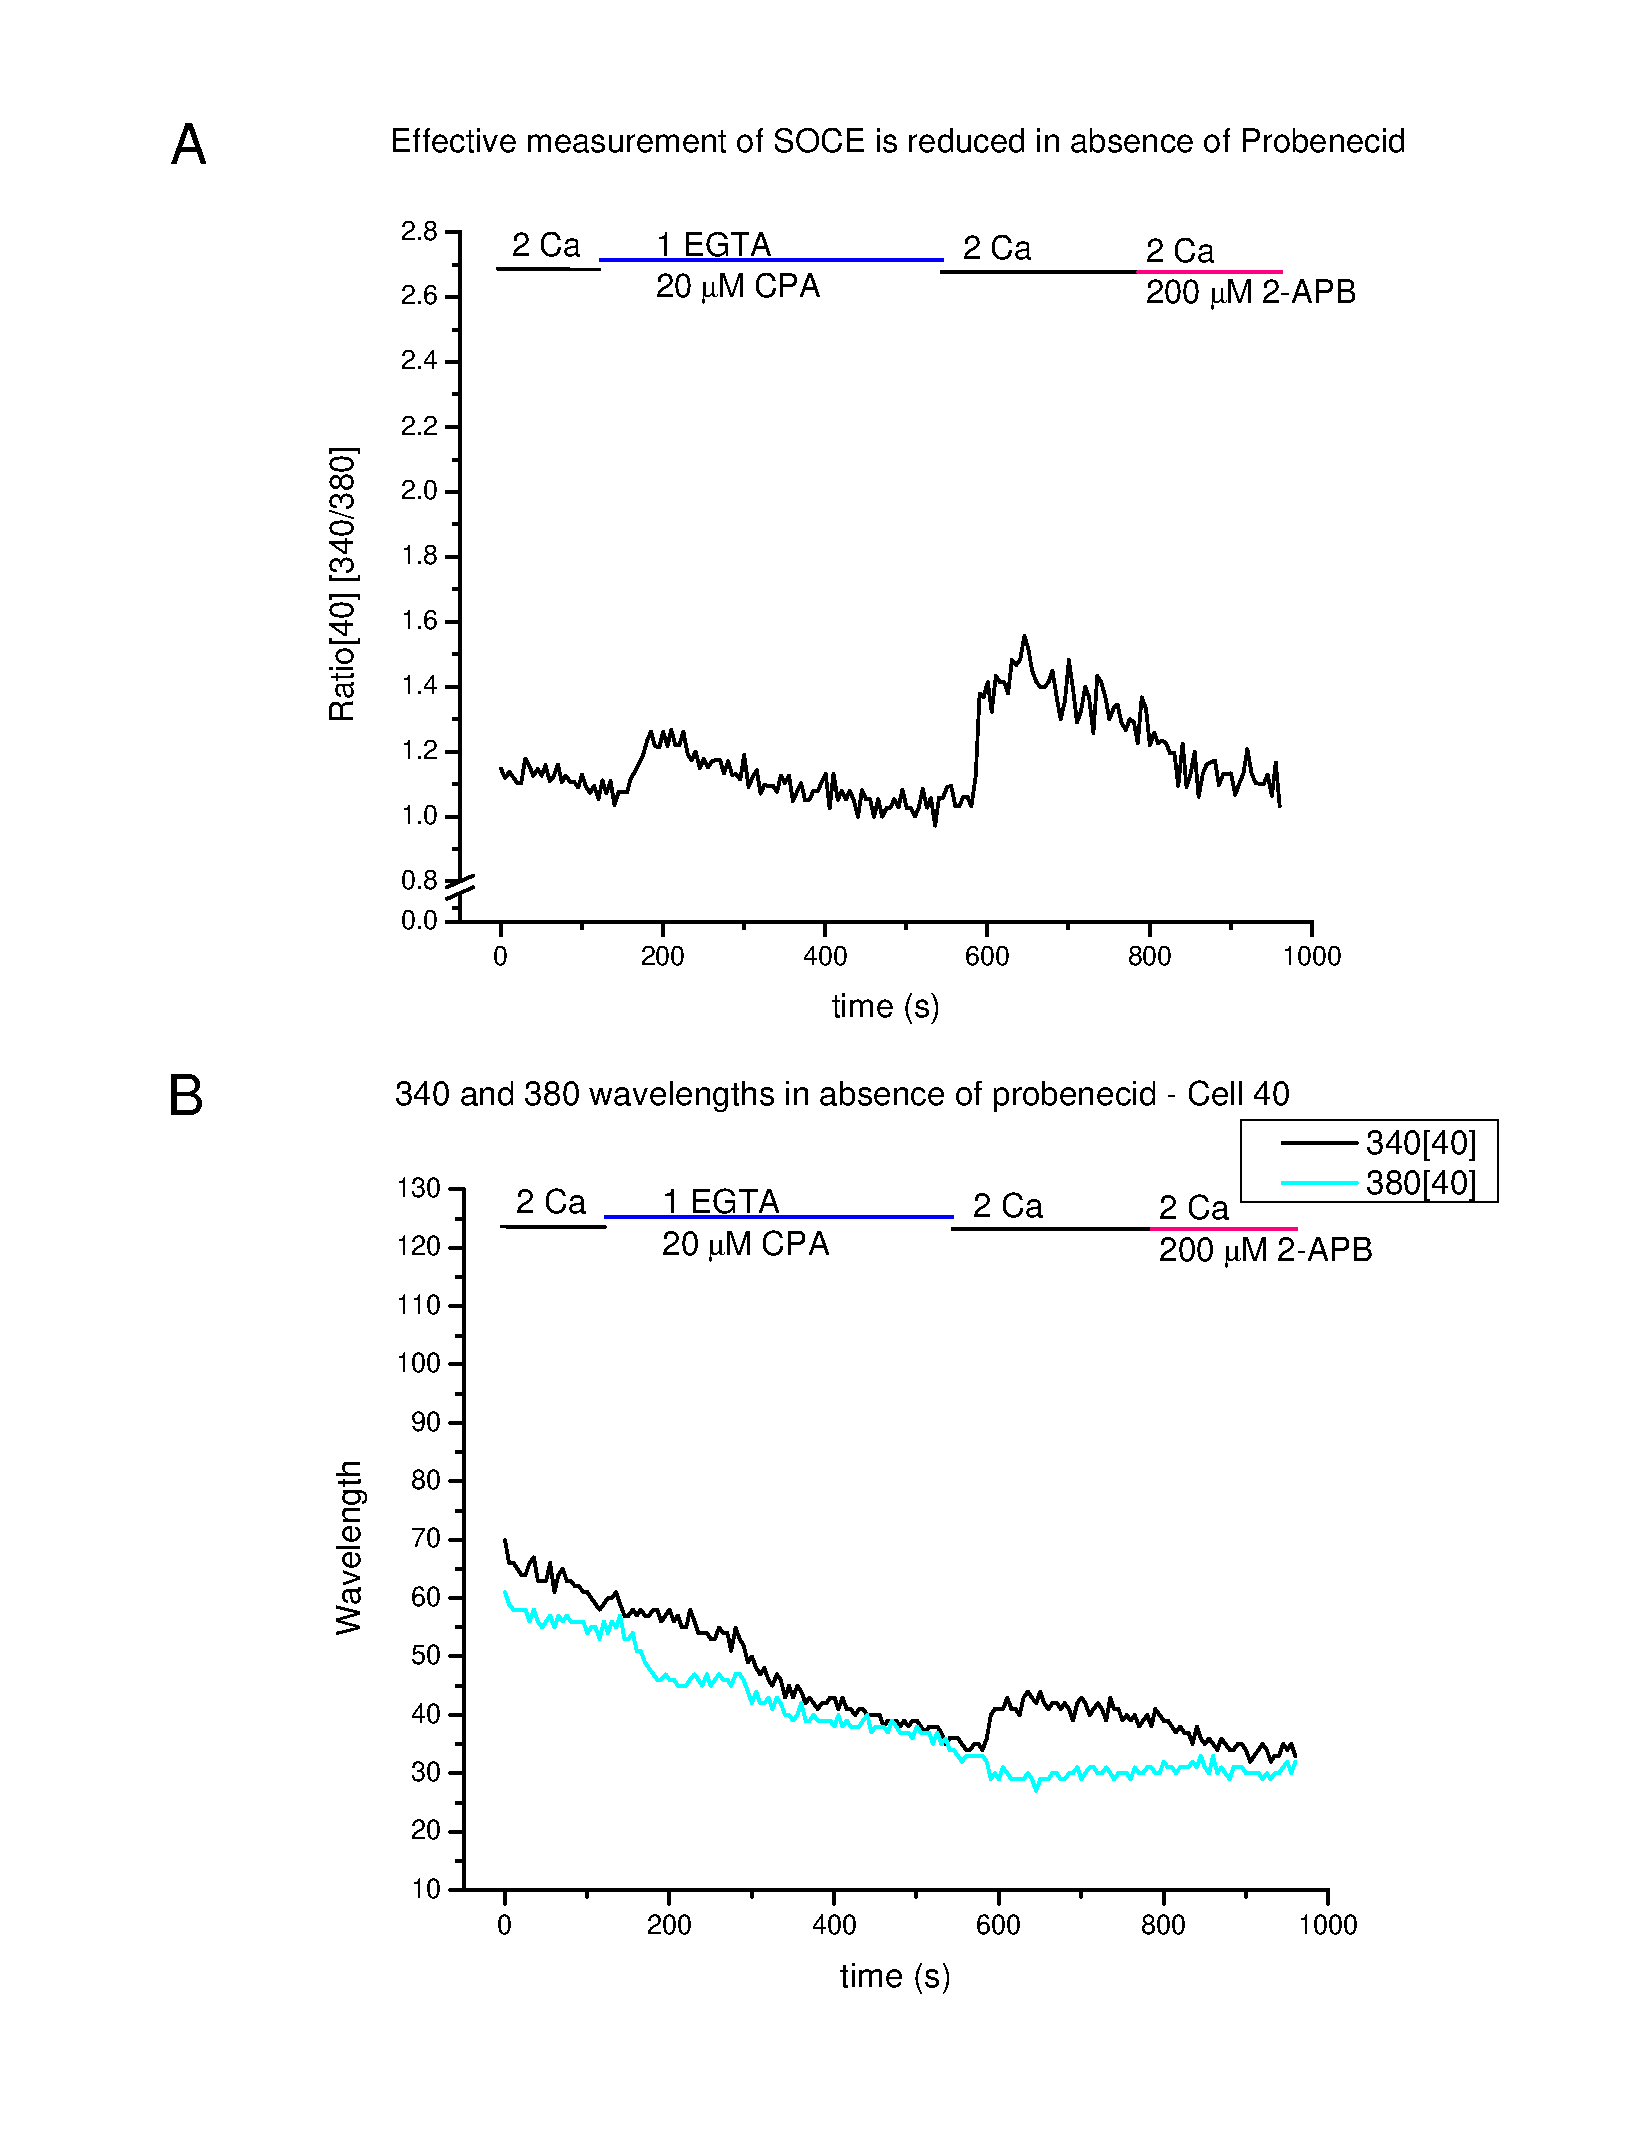
\includegraphics[scale=0.5]{Figures/s2_cell40_nopro.pdf}
\caption[Absence of probenecid gives less efficient dye loading in S2 cells]
	{{\bfseries The absence of probenecid results in less efficient dye loading in S2 cells}. ({\bfseries A}) The ratio of the 340 nm and 380 nm wavelengths of an individual cell during the course of one perfusion experiment where probenecid was omitted from the incubation solution. ({\bfseries B}) The individual 340 nm and 380 nm wavelength values, which produced the ratio seen in {\bfseries A}.}
\label{fig:s2_no_pro}
%\end{center}
\end{figure}

Figure~\ref{fig:s2_no_pro}A shows a recording from an individual S2 cell loaded without probenecid being present in the dye-loading solution (DLS).  Figure~\ref{fig:s2_no_pro}B shows the individual 340 and 380 nm wavelength values that produced the trace in A. Though the trace of the ratio hides it, we see that both wavelengths values start decreasing immediately after the start of the experiment. The decreasing values continue to the end of the experiment. The decay likely reflects leakage of Fura-2 which takes place in S2 cells if probenecid is absent in the DLS \citep{DiVirgilio1990}. The \Ca{} ratios reported after SOCE, upon reintroduction of 2 Ca are  also shown to be low here. This is most likely an artifact caused by less Fura-2 availability, thereby limiting the amount of cytoplasmic \Ca{} that can be measured.

\newpage

\begin{figure}[!ht]
%\begin{center}
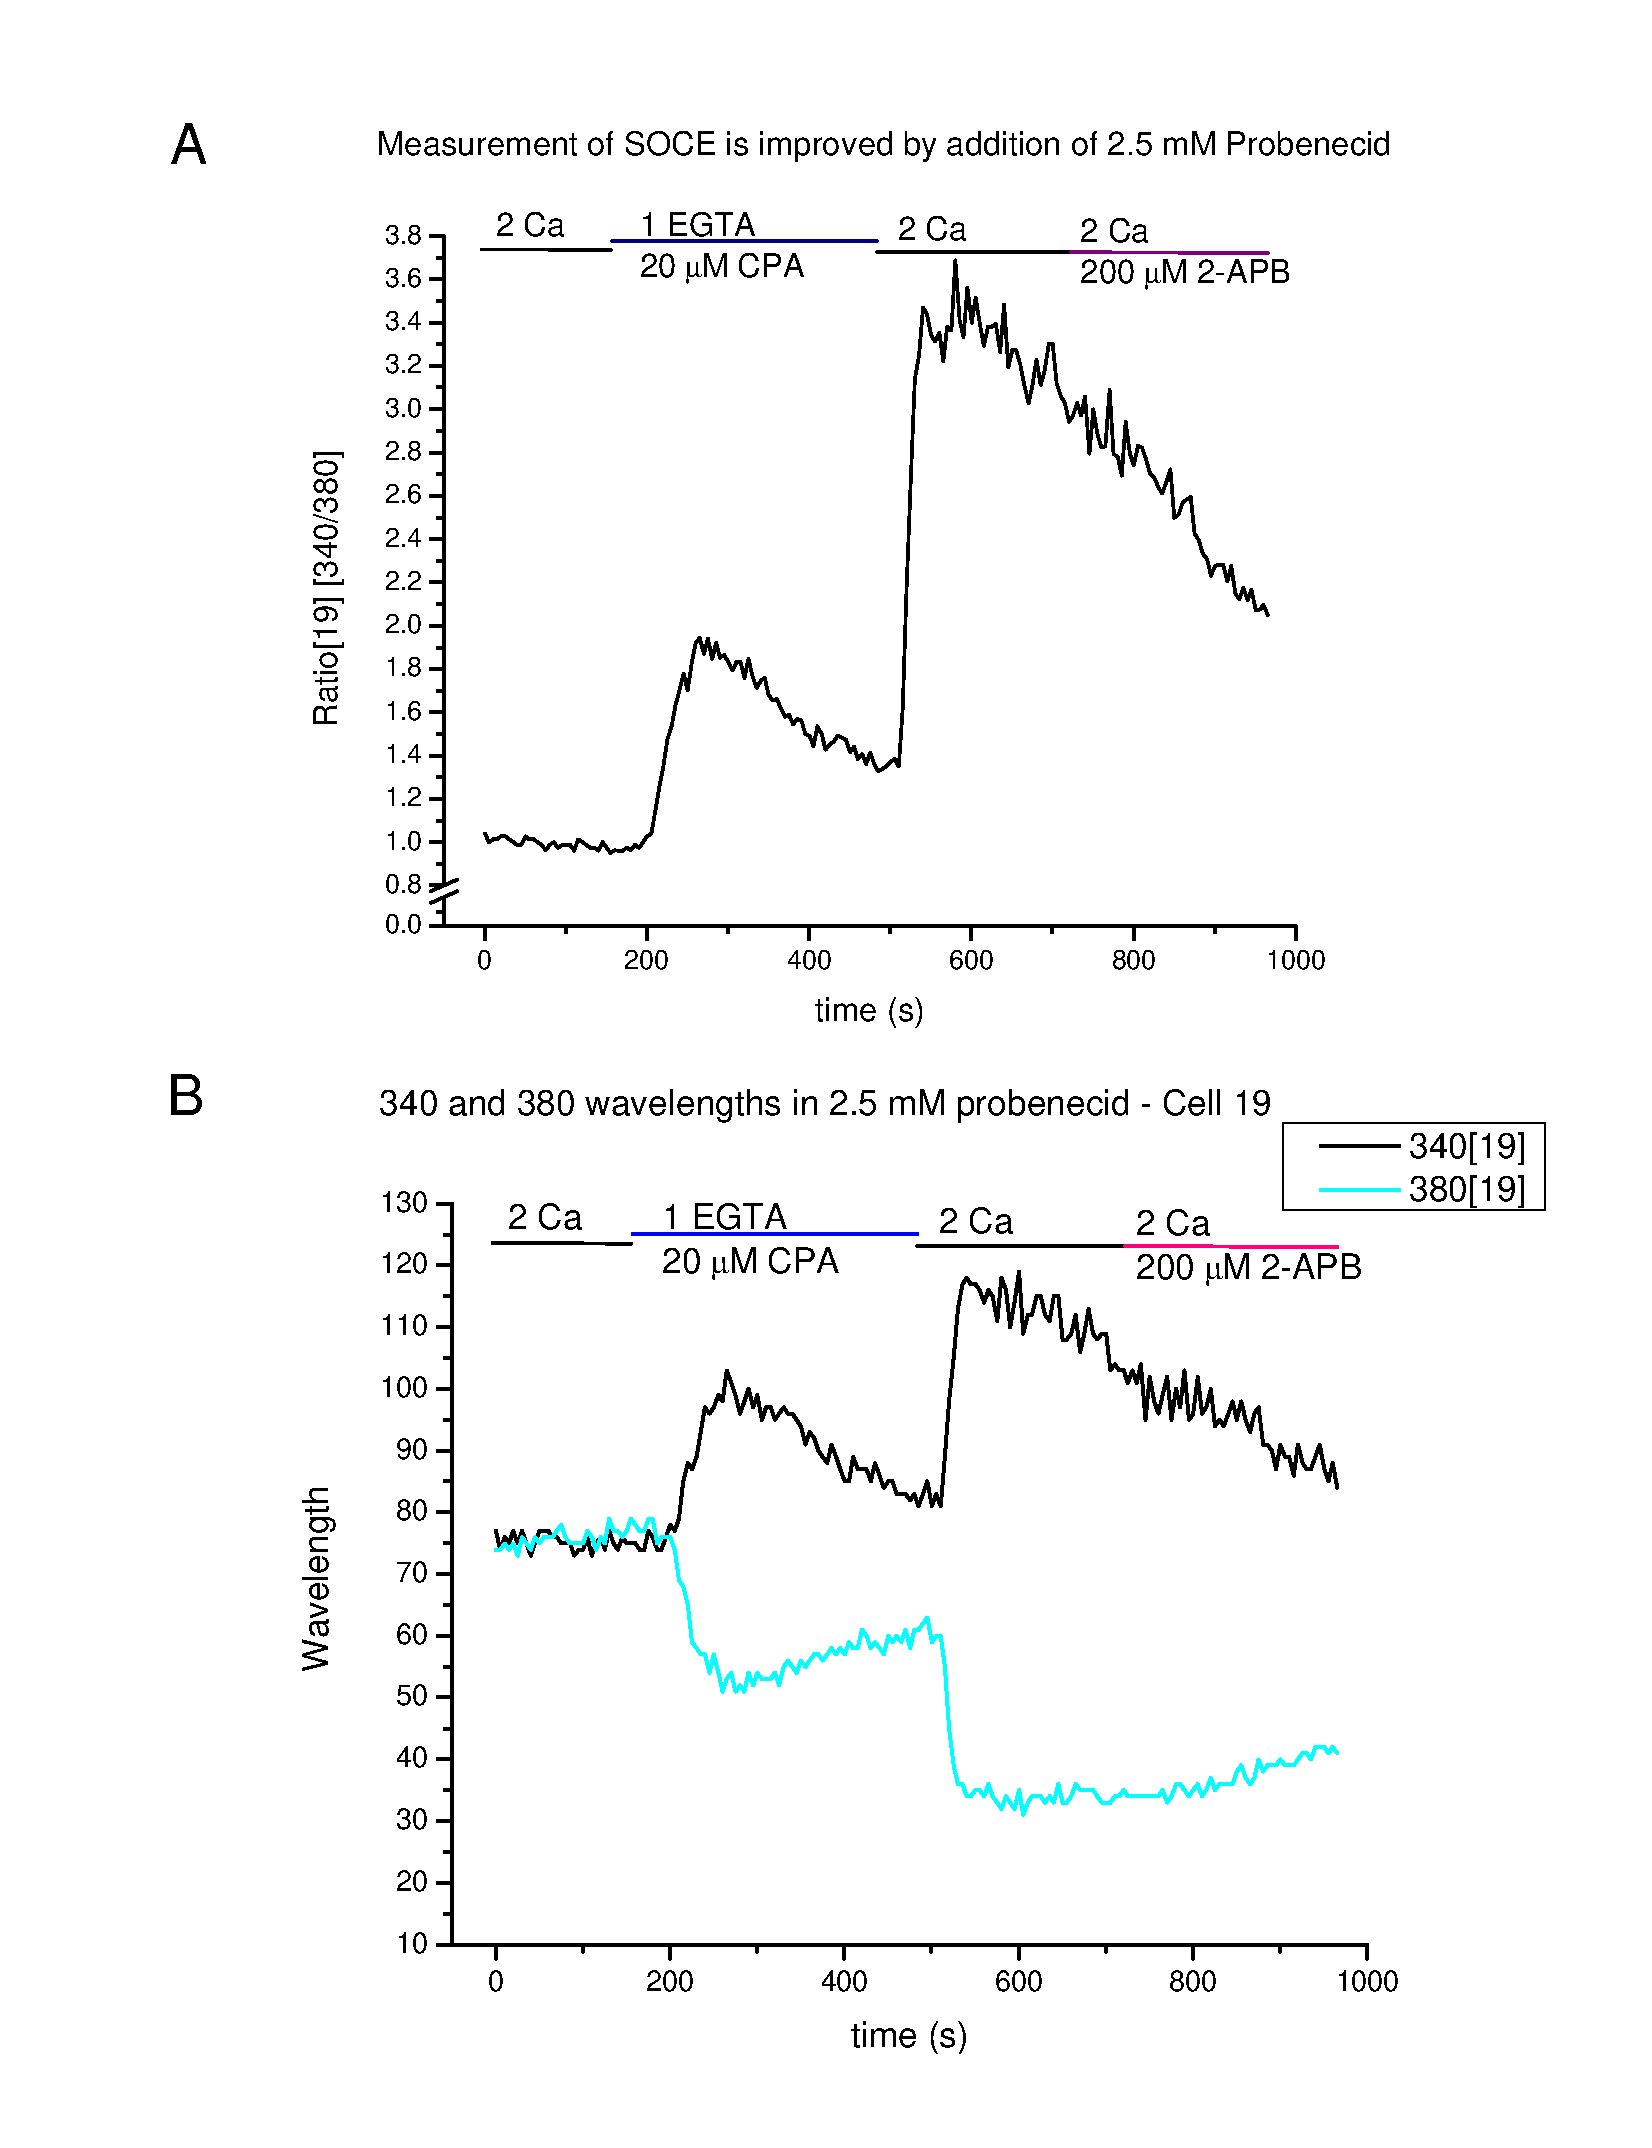
\includegraphics[scale=0.52]{Figures/s2_cell19_pro.pdf}
\caption[Probenecid improves dye loading in S2 cells]
	{{\bfseries The presence of 2.5 mM probenecid improves dye loading in S2 cells}. ({\bfseries A}) The ratio of the 340 nm and 380 nm wavelengths of an individual cell during the course of a perfusion experiment where 2.5 mM probenecid was included in the incubation solution. ({\bfseries B}) The individual 340 nm and 380 nm wavelength values, which produced the ratio seen in {\bfseries A}.}
\label{fig:s2_with_pro}
%\end{center}
\end{figure}

Figure~\ref{fig:s2_with_pro}A shows a sample recording from a cell incubated with DLS containing 2.5 mM probenecid. The ratio is robust and provides better resolution than the trace in figure~\ref{fig:s2_no_pro}. Figure~\ref{fig:s2_with_pro}B gives the individual 340 nm and 380 nm wavelengths which were used to obtain the ratio in A. We are able to clearly see the reciprocal nature of the 340 nm and 380 nm wavelength values. The steady decline of the values over the course of the experiment is no longer apparent. Probenecid has stopped or greatly slowed leakage of Fura-2 from the cytosol. As a result, we are able to record higher \Ca{} transients as more Fura-2 is available as the experiment proceeds, compared to cells loaded without probenecid. This is readily apparent in the SOCE portion of the trace. 

\newpage

\begin{figure}[!ht]
\centering
\subfloat{
	\begin{lpic}[clean]{Figures/no_pro(0.8)}
	%\includegraphics[scale=0.9]{Figures/no_pro} 
		\lbl[bl]{1,105; \bfseries A}
	\end{lpic}
}
	
\subfloat{
	\begin{lpic}[clean]{Figures/with_pro(1.3)}
	%\includegraphics[scale=1.3]{Figures/with_pro}
		\lbl[bl]{6,76; \bfseries B}
	\end{lpic}
}
\caption[Addition of Probenecid improves \Ca{} recordings]{{\bfseries Addition of Probenecid improves \Ca{} recordings}. 
({\bfseries A}) Recordings taken from a population of cells incubated in dye-loading solution that did not contain probenecid ({\bfseries B}) Recordings taken from a population of cells incubated in dye-loading solution that contained 2.5 mM probenecid.}
\label{fig:s2_pro_compare}
\end{figure}

Figure~\ref{fig:s2_pro_compare} shows a population of cells loaded without (A) and with (B) probenecid. We are able to observe a larger \Ca{} transient, due to more Fura-2 being available. Also, addition of probenecid results in more cells meeting the selection criteria for data collection. This can be attributed to Fura-2 retention in probenecid-treated S2 cells. The result is more dye being available at the start of the experiment, and as it progresses. 

Unhealthy cells, cells with damaged plasma membranes may also be omitted from the data set in a reliable, unbiased manner after probenecid treatment. Such cells would still display characteristics of untreated cells such as pronounced, persistent dye leakage.

Conditions for selecting data were formulated after examining individual 340 nm and 380 nm wavelength traces for probenecid-treated and untreated cells. Three out of six cells in A, had either 340 nm or 380 nm wavelength values below 40. This led us to use 40 as a cutoff value for data selection. For the S2 cells selected, both the 340 nm and 380 nm wavelength values stayed at or above 40 during the initial 2 Ca perfusion. This allowed for elimination of cells which were poorly loaded with Fura dye.
%leaky, even after treatment with probenecid  which, for reasons explained above, were deemed undesirable.

%\begin{figure}[htbp]
%\begin{center}
%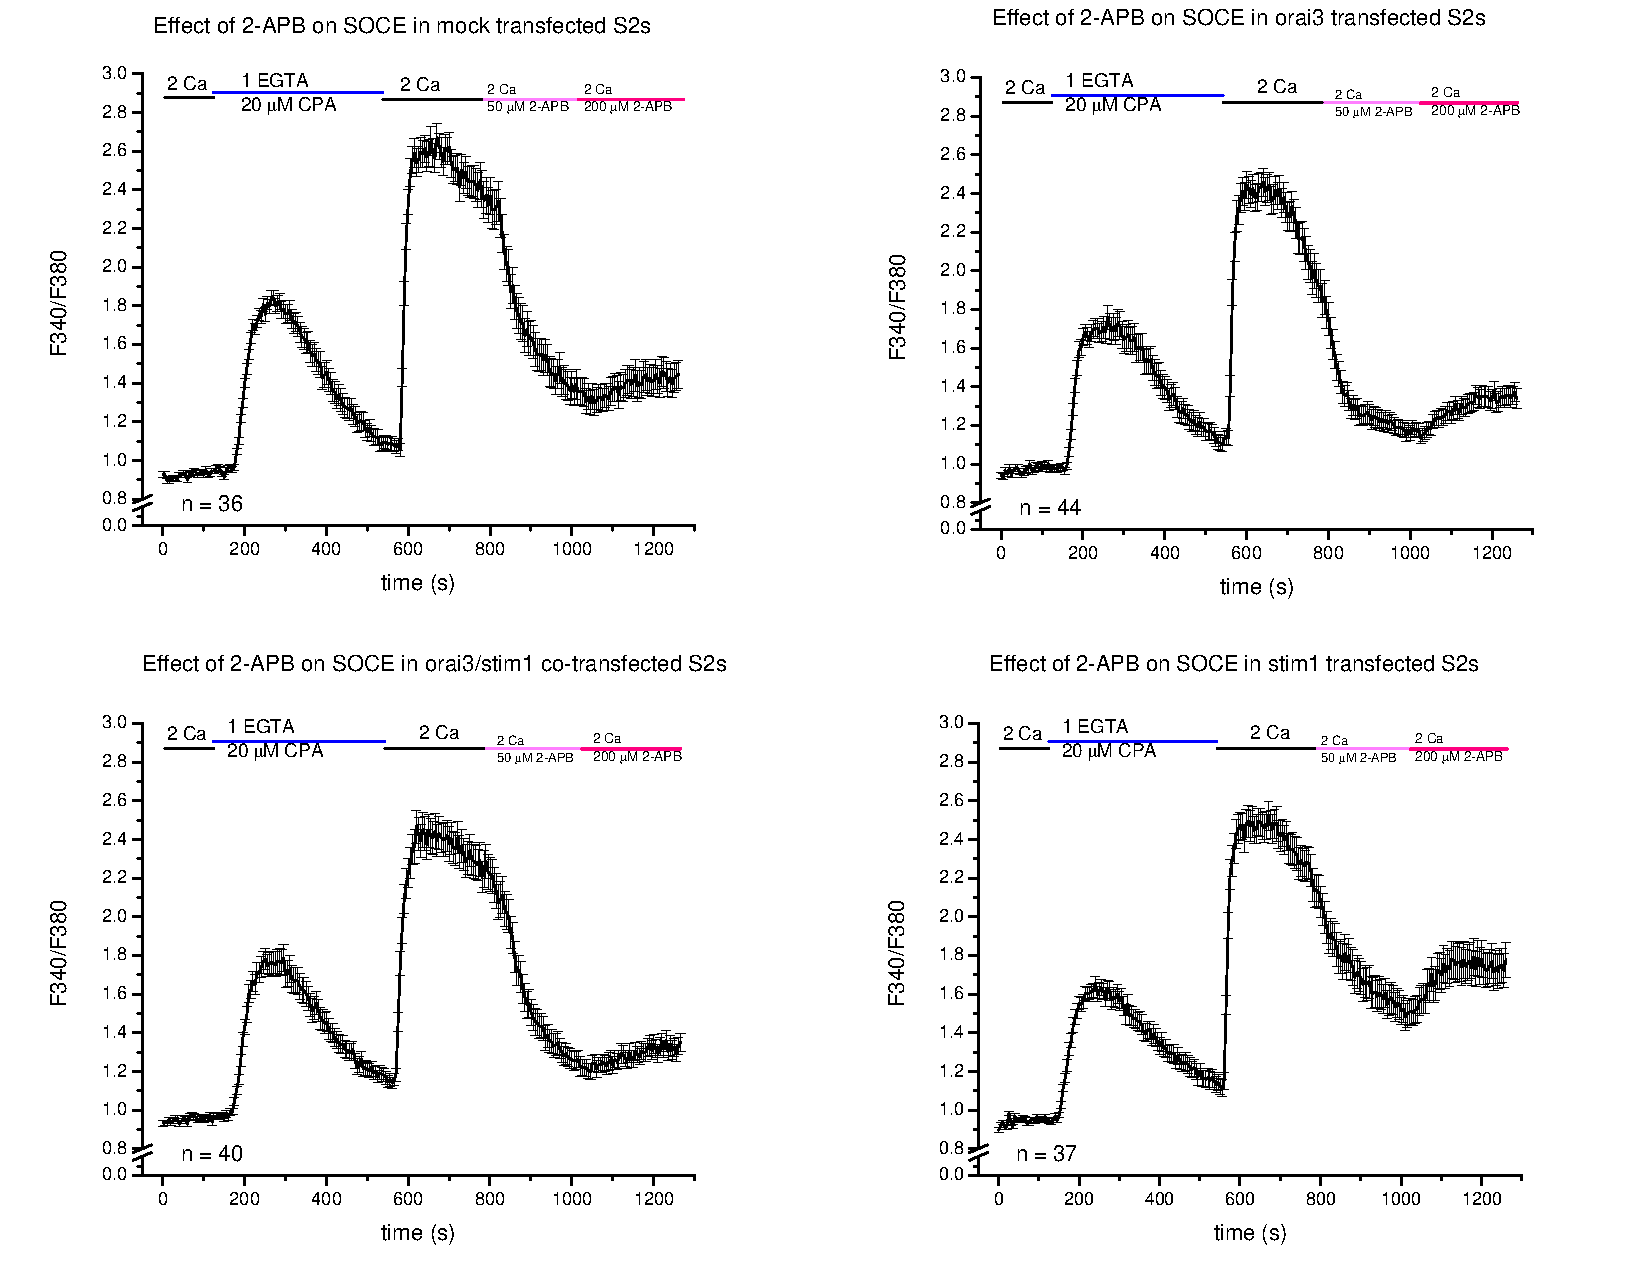
\includegraphics[clip=true, scale=0.61, trim=8mm 0 10mm 0]{Figures/s2_sample_composite}
%\caption{Ca$^{2+}$ measurements in transfected S2 cells perfused with 2-APB}
%\label{fig:s2_composite}
%\end{center}
%\end{figure}
\newpage

\begin{figure}[!ht]
	\centering
	\subfloat{
		\begin{lpic}[clean]{Figures/s2_ca_mock5_all(0.45)}
		%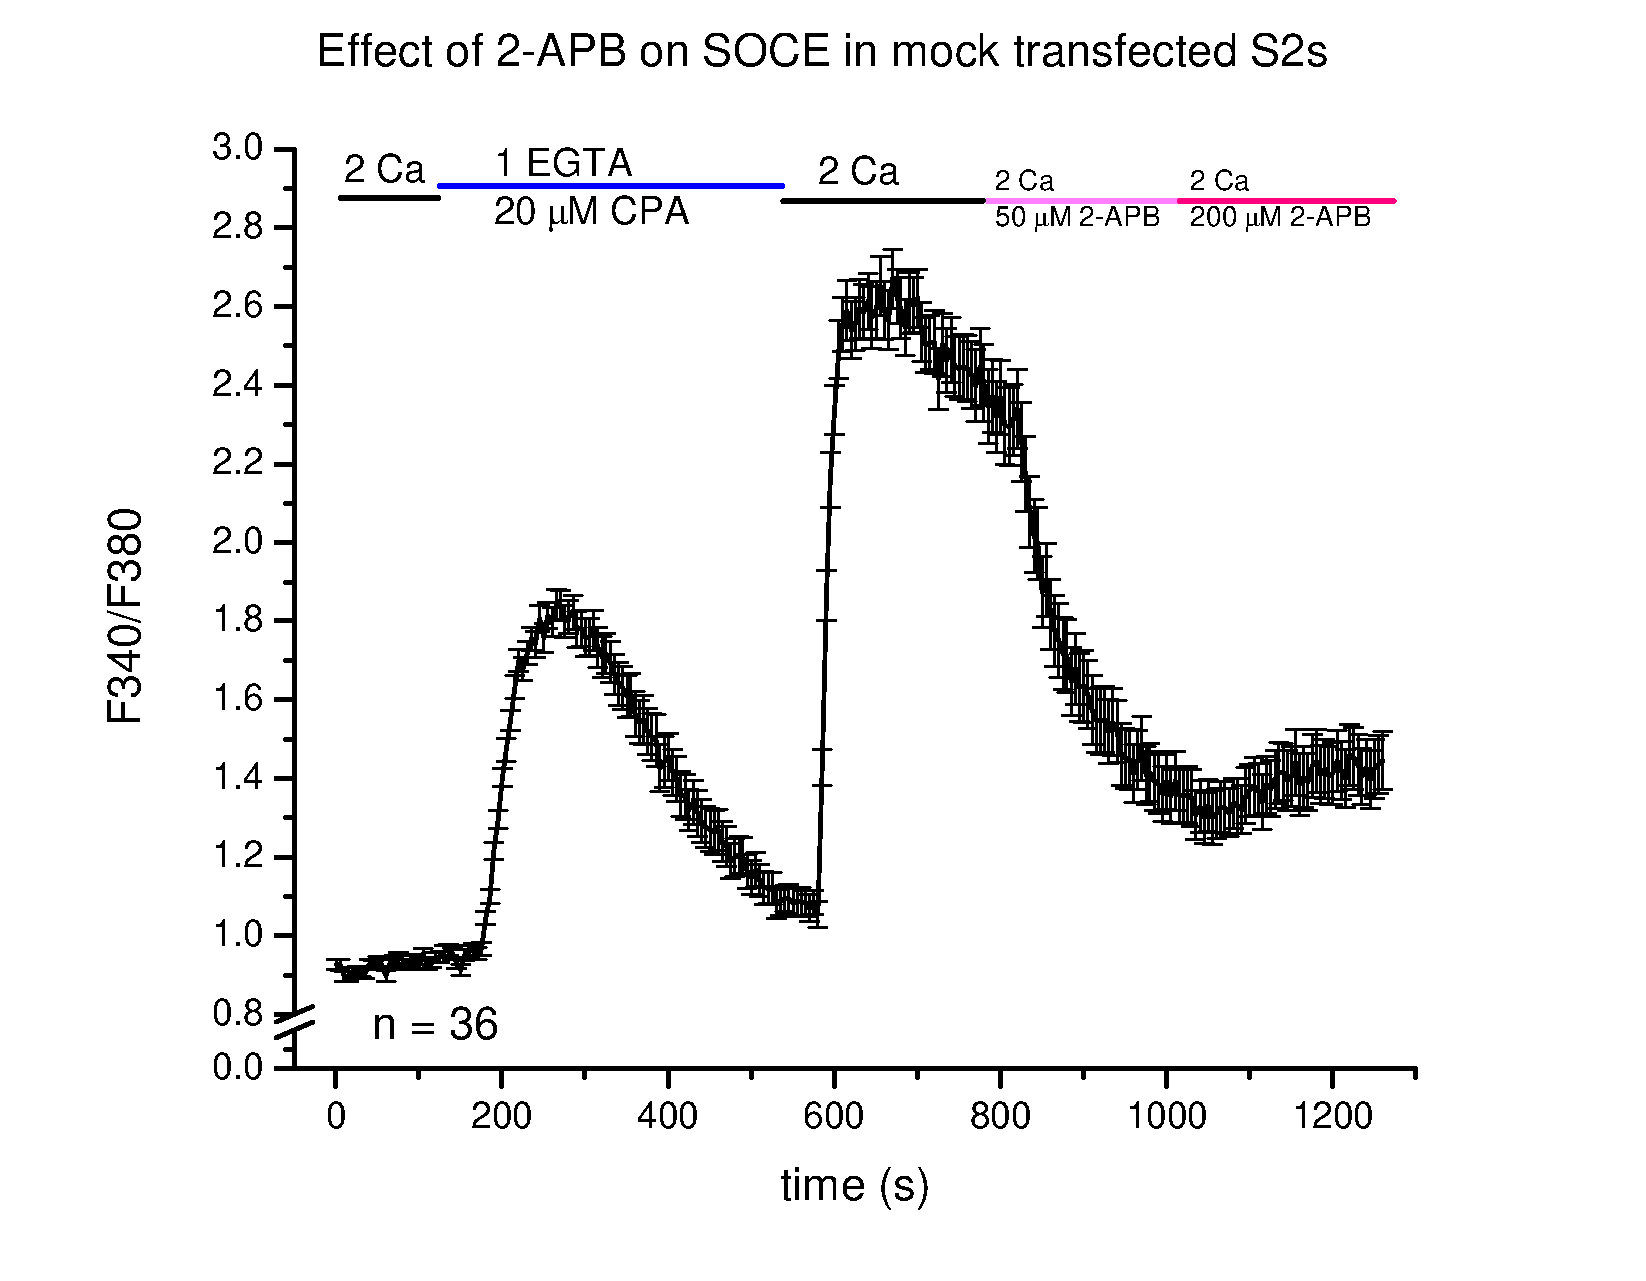
\includegraphics[scale=0.5]{Figures/s2_ca_mock5_all.pdf}
		\lbl[bl]{5,205; \bfseries A}
		\end{lpic}
	}
	
	\subfloat{
		\begin{lpic}[clean]{Figures/s2_ca_orai3_all5(0.45)}
		%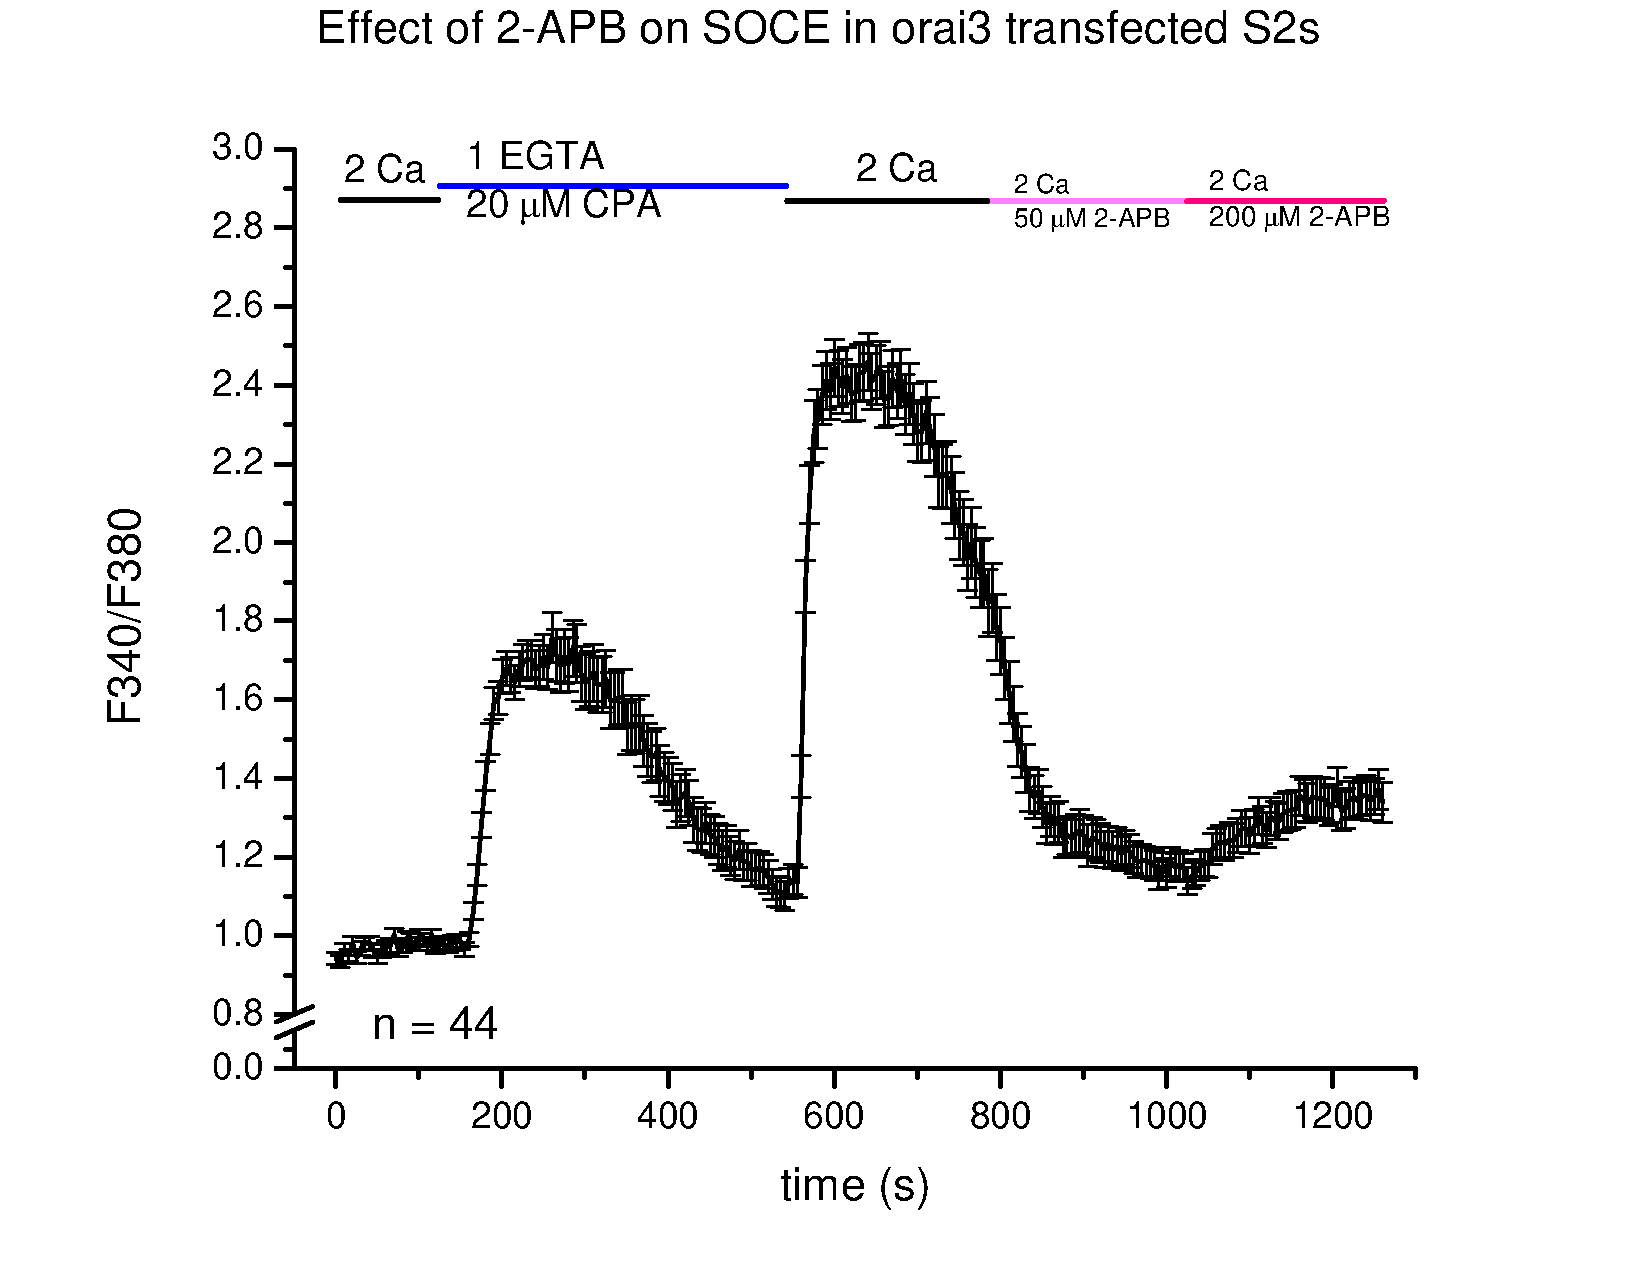
\includegraphics[scale=0.5]{Figures/s2_ca_orai3_all5.pdf}}
			\lbl[bl]{5,210; \bfseries B}
		\end{lpic}
	} 
	\caption[\Ca{} measurements in transfected S2 cells perfused with 2-APB]{{\bfseries \Ca{} measurements in transfected S2 cells perfused with 2-APB}. 	
	The lines above the trace are labeled with the solutions perfused during those times. \textbf{A}) A trace of mock-transfected S2s showing the effect of 2-APB on SOCE. \textbf{B}) A trace of Orai3-transfected S2s showing the effect of 2-APB on SOCE.}
	\label{fig:s2_composite}
\end{figure}
	
\begin{figure}[!ht]
	\centering
	\ContinuedFloat
	\subfloat{
		\begin{lpic}[clean]{Figures/s2_5_o3s1_all(0.42)}
		%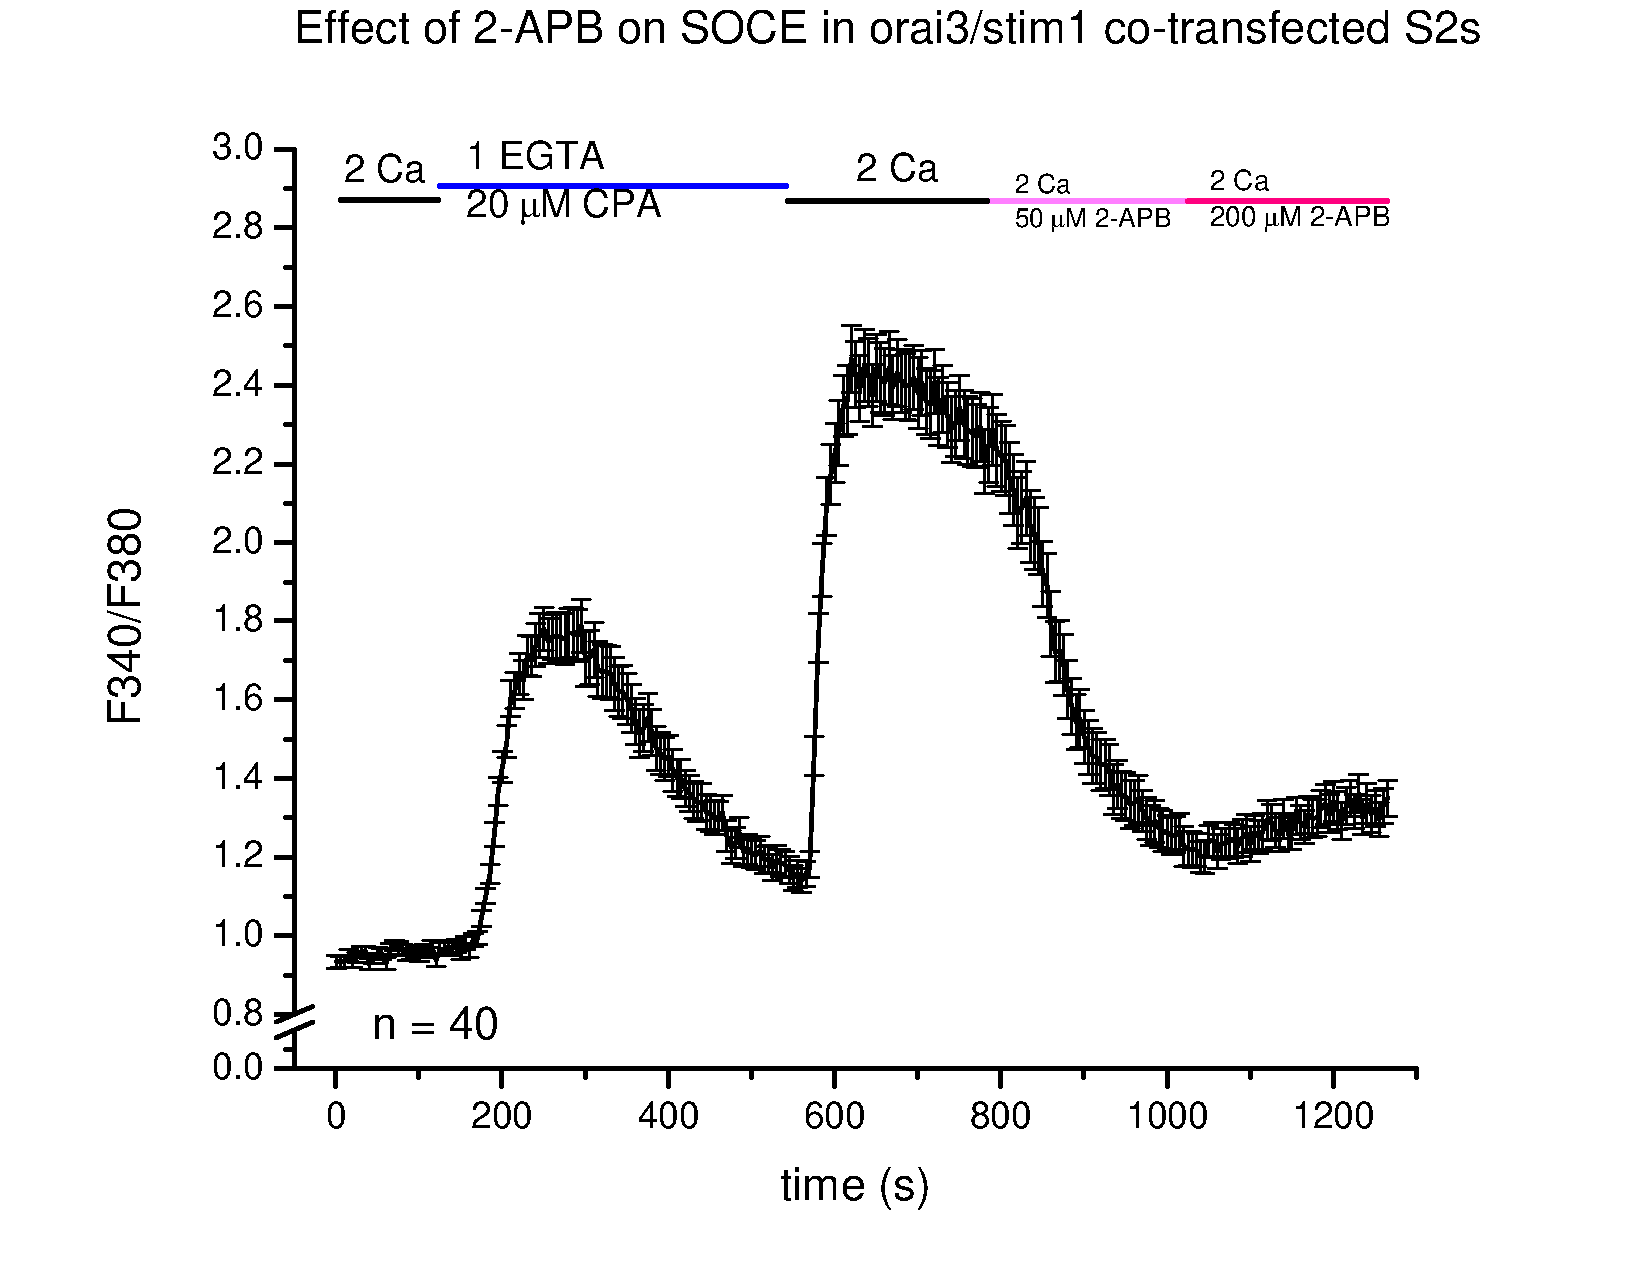
\includegraphics[scale=0.5]{Figures/s2_5_o3s1_all.pdf}
			\lbl[bl]{5,210; \bfseries C}
		\end{lpic}
	}
	
	\subfloat{
		\begin{lpic}[clean]{Figures/s2_ca_stim1_3_all(0.42)}
		%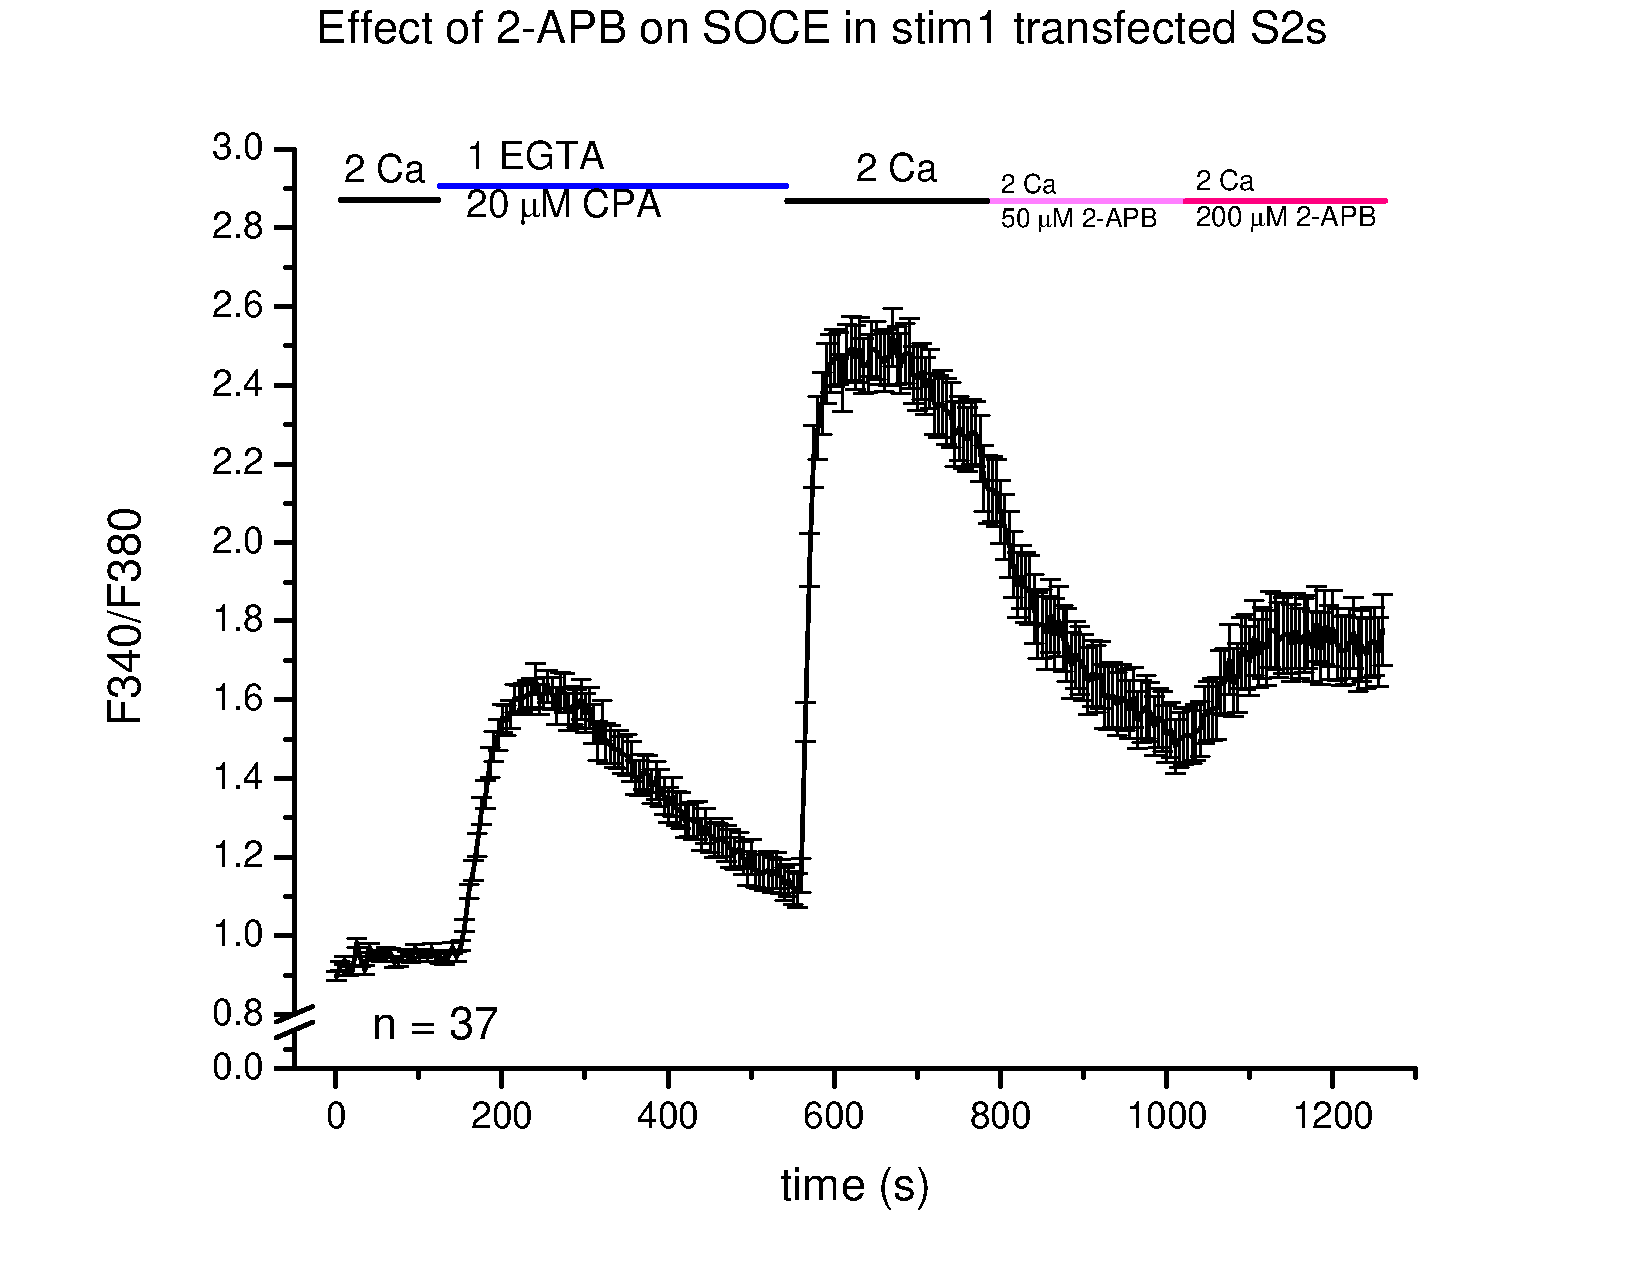
\includegraphics[scale=0.5]{Figures/s2_ca_stim1_3_all.pdf}
			\lbl[bl]{5,210; \bfseries D}
		\end{lpic}
	}
	\caption[]{{\bfseries Ca$^{2+}$ measurements in transfected S2 cells perfused with 2-APB}. 	
	The lines above the trace are labeled with the solutions perfused during those times. \textbf{C}) Sample trace of Orai3+\stim{}-transfected S2s showing the effect of 2-APB on SOCE. \textbf{D}) Sample trace of \stim{}-transfected S2s showing the effect of 2-APB on SOCE.}
	\label{fig:s2_composite}
\end{figure}


The composite in Figure~\ref{fig:s2_composite} shows representative traces for \Ca{} imaging experiments where S2 cells have been mock-transfected or transfected with Orai3, \stim{}, or Orai3+\stim.
In Figure~\ref{fig:s2_composite}A we see an average of several traces giving the result of an experiment done on mock-transfected S2s. Initially, the 2 Ca response of these mock-transfected S2s is relatively stable. Upon introduction of 20 $\mu$M CPA in 1 EGTA, we observe an increase in the F340/F380 ratio. This indicates an increase in cytosolic free \Ca, resulting from leakage of \Ca{} from the ER. This \Ca{} leak achieves a maximum and subsequently declines. The decline phase is indicative of \Ca{} being pumped out of the cell, shuttled to non-ER compartments, such as the mitochondria, or being bound by cytosolic \Ca{} chelators. Transport of \Ca{} to the ER is prevented by CPA, which blocks the SERCA pump. 

After $\sim$7 minutes of perfusion in 1 EGTA/20 $\mu$M CPA, \Ca{} is reintroduced. The mock-transfected S2s then exhibit SOCE, and a second \Ca{} transient forms at this stage. The maximal \Ca{} entry after 2 Ca reintroduction is greater than maximal \Ca{} release from the ER.  \dorai{} channels responsible for SOCE in S2 cells are able to open quickly, allowing \Ca{} into the cell shortly after switching to the 2 Ca solution.
We eventually begin to see less \Ca, which can be attributed to \dorai{} channels closing, slowing \Ca{} entry.

After 4 minutes in 2 Ca, 50 $\mu$M 2-APB is added to the perfusion solution. We see for the mock-transfected S2 cells, that the gradual decline in \Ca{} becomes sharper, shortly after addition of 2-APB. This is expected because at these concentrations 2-APB is inhibitory for \dorai{} \citep{Yeromin:2004p520}. The decline in \Ca{} continues during the 4 minutes in 50 $\mu$M 2-APB. 

After 4 minutes in 2 Ca with 50 $\mu$M 2-APB, the 2-APB concentration is increased to 200 $\mu$M 2-APB. This solution was perfused across the cells for another 4 minutes and then the experiment was stopped. During this time we observe what seems to be a slight increase. The overlap of the error bars along the trace indicate that, while there is a trend toward an increase, further analysis is required to determine its significance. In order to address the question of what happens to \Ca{}, the area under the curve was calculated for each 4-minute section after store-depletion occurred for each group of transfected cells. 

Figure~\ref{fig:s2_composite}B shows an average trace of an experiment performed on Orai3-transfected S2 cells. The initial and store-depletion phases are similar to those in the mock-transfected S2s. 2 Ca reintroduction shows a swift onset of SOCE. The expected increase in \Ca{} after addition of 50 $\mu$M 2-APB was not seen, however. Addition of 200 $\mu$M 2-APB seemed to result in a marginal increase in \Ca{} entry. The \Ca{} content of this 200 $\mu$M 2-APB phase was analyzed further and no significant change from the mock was found (see Figure~\ref{fig:s2_2apb_bar}).

%Discussion: There are a few possibilities for why this happened. The most obvious is that while Orai3 RNA production was induced with \cuso, actual protein production did not occur.Another possibility is that the transfection efficiency was consistently low with the TransIT-2020 reagent and Orai3 vector DNA. This may have resulted in poor expression of Orai3 and a paucity of Orai3 protein translation, leading to a deficiency in Orai3 channels expressed at the cellular surface. Another possibility is that, because of how closely related Orai3 and \dorai{} are, Orai3 forms heterodimers with \dorai, and adopts a phenotype primarily \dorai{} in nature.
%Testing protein expression of Orai3 proteins is possible, by isolating proteins from cells and performing a Western Blot using antibodies purchased to Orai3. 
%The generation of stable cell lines expressing Orai3 will facilitate experiments important for testing the other possibilities. \rnai{} knockdown of native \dorai{} will enable these experiments to be carried out in a background free of Orai which may be interfering with our heterologous Orai3 channel assembly. 

Since no distinct effect of 2-APB was observed in S2s transfected with Orai3 only, Orai3+\stim{} transfections were performed. We reasoned that human Orai3 may require a human \stim{} protein for coupling, rather than the background \dstim{} natively expressed in S2 cells. A trace for one of these experiments is provided in Figure~\ref{fig:s2_composite}C. 
The store-depletion and SOCE phases again seem similar to that of the mock- and Orai3-transfected cells. When treated with 50 and 200 $\mu$M 2-APB, no clear trend was visible compared to the mock- or Orai3-transfected cells.

In Figure~\ref{fig:s2_composite}D a similar experiment was performed, but on \stim{}-transfected  S2s. 
Here, the store-depletion and SOCE phases after 2 Ca reintroduction are similar to mock and other transfections. Interestingly, addition of 50 $\mu$M 2-APB in the \stim{} only transfected cells, was less effective at slowing \Ca{} entry than in the other transfections. %There seemed to be less deactivation of the \dorai{} occurring compared to the mock transfection. An alternative explanation is that another channel which allowed Ca{} into the cell was opening up due to the presence of \stim{} and 2-APB. 
When 200 $\mu$M 2-APB was added, a clear increase in cytosolic \Ca{} was observed.



\newpage

\begin{figure}[htbp]
\begin{center}
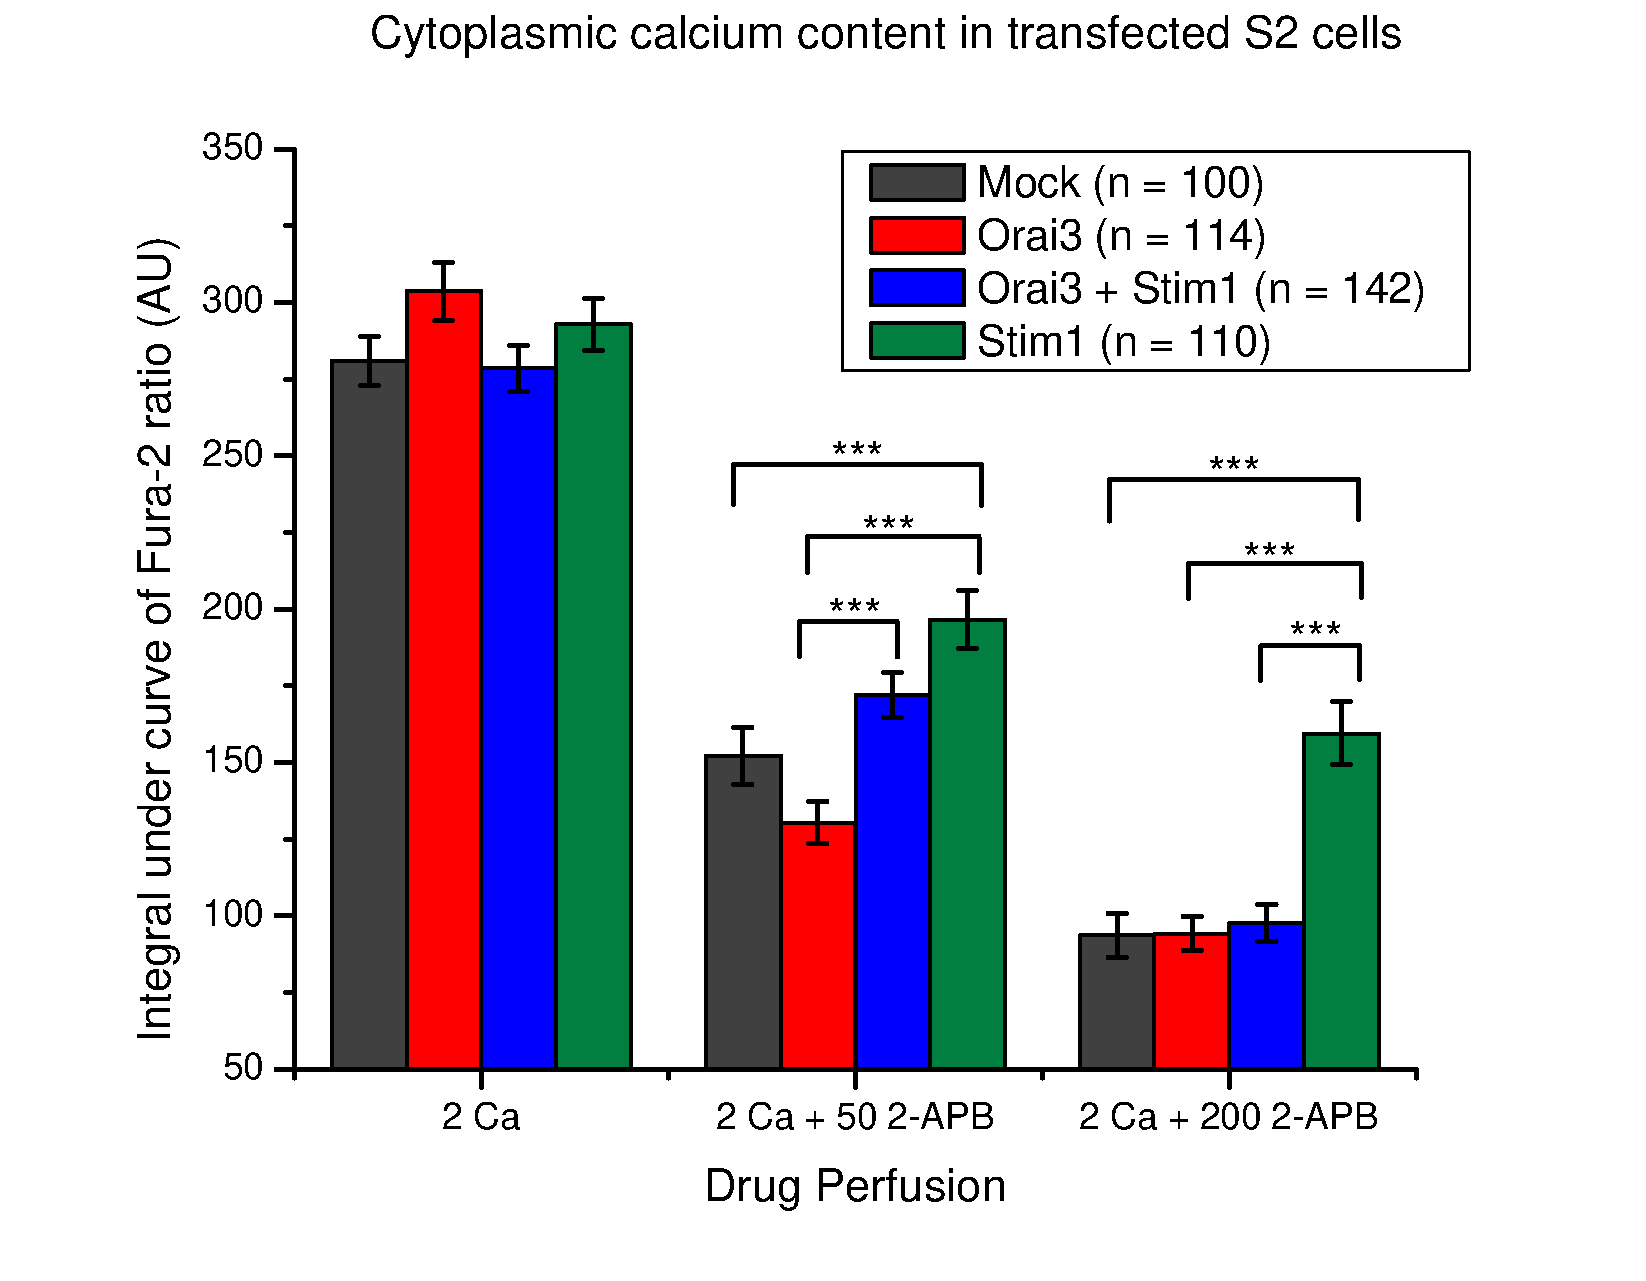
\includegraphics[clip, trim = 0 0 25mm 20mm, scale=0.6]{Figures/s2_drug_bar}
\caption[Cytoplasmic \Ca{} content in transfected S2 cells]{{\bfseries Cytoplasmic \Ca{} content in transfected S2 cells}. 
The bars represent area under the curve analysis for segments where {\bfseries 2 Ca}, {\bfseries 2 Ca + 50 $\mu$M 2-APB}, or {\bfseries 2 Ca + 200 $\mu$M 2-APB} were used to perfuse transfected S2 cells. The transfection groups are indicated in the legend. Significant differences between the transfected groups at the 0.05 significance level are indicated by ***. No significant difference was found between the 2 Ca perfusion group. Significant differences were found between the 2 Ca + 50 $\mu$M 2-APB and 2 Ca + 200 $\mu$M 2-APB perfusion groups.}
\label{fig:s2_2apb_bar}
\end{center}
\end{figure}

Figure~\ref{fig:s2_2apb_bar} displays the results of area under the curve (AUC) analysis on the three phases of treatment after store-depletion. By doing AUC analysis, the ratios generated by Fura-2 recordings were translated into cytosolic \Ca{} content of arbitrary units. The three groups in the bar graph correspond to perfusion with 2 Ca, 2 Ca + 50 $\mu$M 2-APB, and 2 Ca + 200 $\mu$M 2-APB. The perfusion time for each group was 4 minutes. A one way ANOVA was used to determine if there were significant differences in the experimental groups. If significant differences were found, Tukey's \underline{studentized} range test, was used to determine where significant differences lie between the transfection groups.  

The 2 Ca group represents an untreated period of SOCE in the transfection groups. Statistical analysis showed no significant change in cytosolic \Ca{} for this group. Functional Orai3 \Ca{} channels were expected to increase the levels of cytosolic \Ca{} during SOCE. 
%That this was not observed may be due to the \Ca{} capacity of the cell already being at maximal levels. If the S2 cell is capable of holding a finite amount of \Ca{}, and it had already reached that point, more \Ca{} channels would merely get it to that point faster, but observing further increase in \Ca{} levels would not be expected in this case.
That this was not observed may be due to the inability of Orai3 to express \emph{in the membrane}, a possibility addressed in the discussion. 

%Discussion mock:
%To determine whether the cell's cytosol was at its maximal \Ca{} carrying capacity, experiments with 2 Ca and ionomycin can be performed. After store depletion with CPA, 2 Ca can be perfusion, followed by a 2 Ca + ionomycin solution. Ionomycin is an ionophore which would raised the   \cai{} to that of the external solution. Depending on the result of perfusion with 2 Ca + ionomycin, we could say with certainty whether the maximal \Ca{} carrying capacity of the cytoplasm was reached. If for example, perfusion with ionomycin resulted in higher Ca{} levels, than was obtained without ionomycin, this would indicate that maximal levels were not obtained. 
%Discussion
%Another method for determining this would be to change the concentration of \Ca{} being used in the perfusion solution. All solutions contained 2 mM \CaCl, but decreasing the concentration to $\mu$M levels, which provide less \Ca{} for SOCE. This would result in less Ca{} being available for entry and a lower cytosolic calcium content resulting. If the \Ca{} from SOCE was still not significantly different between the transfection groups, this would allow us to conclude that the Orai3 channels were not activated solely as a function of store-depletion.


The 2 Ca + 50 2-APB experiments did show significant differences in this treatment group. 
Significant differences existed between Orai3+\stim{}-transfected cells and the Orai3 only transfected group. There were also significant differences between \stim{} only transfected cells and Orai3 only transfected cells. For both of the groups described above, the Orai3 only group showed much less cytosolic \Ca, which was unexpected. 
A significant difference was also found between mock-transfected and \stim{}-transfected cells, with the \stim{}-transfected group having higher levels of cytosolic calcium than the mock-transfected group.
The significant differences for all of the above was p $<$ 0.0001 at the 0.05 significance level. 

%Discussion:
%When only Orai3 was transfected into S2 cells and perfused with 2 Ca + 50 2-APB, a slight decrease was observed compared to mock-transfected cells, though this was not found to be significant. There were significant differences between Orai3 only and two other transfected groups: Orai3 + \stim{} and \stim{} only. That there was \emph{less} \Ca{} available in Orai3 only transfected cells, suggests that the effect of 2-APB on these  was inhibitory.
%This is supported by the finding that only \stim{}-transfected cells had significantly higher cytosolic \Ca{} than the mock-transfected cells. The difference between Orai3+\stim{} and Orai3 only transfected cells, is likely the result of the action of heterologously expressed \stim{} in this DES.


The 2 Ca + 200 2-APB showed a small but significant difference only between the \stim{}-transfected  cells and all the other groups. Again, an unexpected result which is discussed further below.  


%The \stim{} + 2-APB interaction is enhanced in higher concentrations of 2-APB. The overexpression of \stim{} in this DES may be resulting in opening of another channel by heterologous \stim{}, or alternatively slowing the deactivation of the \dorai{} responsible for the SOCE. We can see if this effect of \stim{} is specific to SOCE, by performing a similar experiment, but omitting the store depletion portion. In the absence of store-depletion, there should be no activity by \dorai{} thus any \Ca{} entry observed would likely be due to another channel. We could also test using inhibitors known to affect \dorai, such as (Ln3+?)(CITE) to determine whether the \dorai{} is being activated by \stim{} here, because \stim{} somehow changes some the characteristics of the channel. e.g. if heterologously expressed \stim{} is in the membrane, and 2-APB activates it without the need for heterologous ER \stim{} to act.

%************************

%note that perfusion of s2 cells results in near instantaneous changes in ca recordings. 
%each segment is 4 minutes long. 
%mention tukey's stat analysis
%look at probenecid - hammer that home. want to use probenecid.
%in discussion, stim1 possibilities. this vs. that.  
%Maybe Orai3 in S2s will activate in absence of store depletion.




% -eof-


 
\chapter{Introduction}
%In 1983, 
Two key articles published in the 1980's defined the new phenomenon of store-operated calcium entry (SOCE): \citet{Streb:1983p278} showed that stimulation with inositol (1,4,5)-trisphosphate (IP3) triggered calcium (\Ca) release from the endoplasmic reticulum (ER) and soon after, %Later, in 1986, 
\citet{Putney:1986p283}, proposed that depletion of intracellular \Ca{} concentration (\cai) signaled the plasma membrane \Ca{} entry channels to open \citep{Taylor2006}. These and other
early studies %in macrophages and Jurkat cells 
\citep{Hoth:1992p527,Zweifach1993} formed the framework for subsequent investigations of \SOCE{} in various cell types. Initially, the more popular term used was capacitive calcium entry (CCE). Over 20 years later, other major players in this story were revealed. Stromal interaction molecule 1 (STIM1), was found to affect SOC influx in an RNA interference (\rnai) based screen and identified as the ER calcium sensor \citep{Roos2005, Liou2005, Zhang2005}. Shortly thereafter the store-operated calcium channel, Orai1, was identified \citep{Feske2006, Prakriya2006, Vig2006, Zhang2006, Smyth2010}. 

There are two mammalian homologs of Orai1 -- Orai2 and Orai3 -- whose functions are not yet fully understood \citep{Roos2005,Vig2006,Taylor2006,Smyth2010}. It is possible that Orai2 and Orai3 are expressed in a tissue-specific manner. This seems to be the case with estrogen receptor-positive (ER+) breast cancer cells, which have been shown to use Orai3 as their store-operated \Ca{} channel \citep{Motiani2010, Dellis2011}. The demonstrable involvement of Orai3 in a disease state as prevalent as breast cancer, underscores the importance of further studies of these Orai channels whose function in the body is not yet understood. The presented study sets the foundation for pharmacological characterization of the Orai3 \Ca{} channel, using \droso{} S2 cells as a heterologous expression system. This system is expected to be of more general use for physiological and pharmacological studies of all Orai channels. We begin by introducing calcium signaling through store-operated channels in non-excitable cells. 



\section{Background}


\subsection{Calcium Signaling}
%Ultimately we will be looking at the effect which 2-APB has on Orai3, using cellular \Ca{} elevations as our output.   
\Ca{} is an incredibly versatile signaling molecule, affecting all parts of the cellular signaling machinery. \Ca{} signaling is critical to such processes as exocytosis, transcription, cardiac function, mitosis and apoptosis \citep{Berridge2003,Berridge2000,Gwack2007,Smyth2010}. 
The speed of these processes range from seconds to days \citep{Berridge2003}. 

Since \Ca{} can enter the cell's cytoplasm by influx at the plasma membrane or release from internal stores, such as those within the ER \citep{Berridge2003,Berridge2000,Smyth2010}, it is necessary to maintain a balance between the two pathways. This is to prevent \Ca{} from accumulating where it should not, which would activate or deactivate cellular processes at inopportune times. 
\Ca{} concentration is regulated through activation of different  ion channels.
The most studied \Ca{} ion channels in the ER are the IP3 and ryanodine receptors  (IP3R, RYR) \citep{Berridge2000, Lewis2001, WPutney:2006p130}. These channels are activated by %additional 
second messengers. %The IP3R is activated by IP3 which opens the channel, allowing release of ER \Ca{} into the cytoplasm.

``On'' mechanisms are the means by which \Ca{} is released from internal stores into the cytoplasm. ``On'' mechanisms depend on \Ca{} channels \citep{Berridge2000} which may be voltage-operated channels (VOCs), receptor-operated channels (ROCs), and/or store-operated channels (SOCs) \citep{Berridge2000}. 


``Off'' mechanisms also exist to quickly lower \cai, and this is done through various pumps and exchangers \citep{Berridge2000}. The plasma membrane \Ca -ATPase and Na$^+$/\Ca{} exchanger (if present)  move \Ca{} out of the cell, while the sarco-endoplasmic reticulum \Ca{} ATPase (SERCA) will pump \Ca{} back into the ER, replenishing the cell's internal stores \citep{Berridge2000}.

Orai1, the recently identified Calcium-Release Activated Calcium (CRAC) channel, is a store-operated \Ca{} channel \citep{Prakriya2006, Vig2006, Feske2006, Zhang2006, Smyth2010}. 
Orai3 is closely related to Orai1 \citep{Feske2006, Taylor2006, Gwack2007}, and is thought to be involved in store-operated calcium entry (SOCE). According to the Basic Local Alignment Search Tool (BLAST), Orai3 has 58\% nucleotide sequence homology with Orai1. 
%It is necessary then to understand the role that \Ca{} plays in this process.
When SOCs open they allow \Ca{} into the cytosol. This leads to \cai{} increasing from nanomolar to micromolar levels \citep{Berridge2000}. This \Ca{} is both stimulatory and inhibitory \citep{Berridge2000} since this ion acts as a signal for such a wide array of cellular processes. Spatial regulation becomes very important in allowing for control of stimulatory and inhibitory \Ca-dependent mechanisms. \Ca-binding proteins act as buffers and allow the cell to control the local \cai. Cytosolic \Ca{} buffers such as parvalbumin, calbindin-D, and calreticulin, along with \Ca{} pumps and exchangers are important in regulation of \cai{} \citep{Berridge2000}. 
The affinity which these buffers have for \Ca{} is also important. Parvalbumin, for example, has a high affinity for \Ca{} but slower binding kinetics than calbindin-D and calreticulin \cite{Berridge2003}. The different \Ca{} binding affinities allow for buffers which can modify amplitude, recovery time and diffusional range of \Ca{} %transients 
\cite{Berridge2003}. 


In addition to their buffering capacity, cytosolic \Ca{} binding proteins can also act as  \Ca{} sensors \citep{Berridge2000}.  \Ca{} sensors, such as troponin C, calmodulin, phospholipase C 
% PLC has 4 EF-hands motifs for binding Ca2+
and recoverin respond to changes in \cai. They do so with the aid of %four
 EF hand motifs and will bind \Ca{} to undergo conformational changes, and then activate downstream processes \citep{Berridge2000}. This mechanism of detecting changes in \cai{} should be emphasized, as it will become relevant for another player in the SOCE mechanism, \stim.

\subsection{Store-Operated Calcium Entry}

SOCE is an interesting, yet simple process. Broken down to its simplest form, it is a process which signals for \Ca{} to be allowed into the cell when more is needed \citep{Putney:1986p283,Berridge2000,Lewis2001}. SOCE is triggered by the loss of \Ca{} from the cell's own internal ER \Ca{} stores. ER \Ca{} sensors detect the loss of \Ca{}, migrate close to the plasma membrane (PM), and signal PM \Ca{} channels to open. This further increases the \cai{} and allows for replenishing the stores \citep{Taylor2006}, as well as providing \Ca{} necessary for various cellular processes \citep{Berridge2003,Berridge2000,Gwack2007,Smyth2010}. % A good analogy for the process would be flushing a toilet bowl. The toilet is flushed and water, analogous to \Ca, is depleted. This results in an influx of water from an external reservoir (extracellular environment). Our water will then move along a pipe, signifying our \Ca{} channel, from our external environment, eventually refilling the toilet bowl. 

Store-operated \Ca{} channels in lymphocytes are responsible for \Ca{} entering from extracellular fluid (i.e. blood) \citep{Lewis2001,Berridge2000, Gwack2007}, and lack voltage-sensitive \Ca{} channels \citep{Lioudyno2008}. T-cell receptor engagement activates the enzyme phospholipase C gamma (PLC$_\gamma$). PLC$_\gamma$ will then  hydrolyze phosphatidylinositol 4,5-bisphosphate (PIP2) in the membrane resulting in soluble IP3, and membrane-bound diacylglycerol (DAG) \citep{Berridge2000,Lewis2001}. IP3 binds to IP3R opening it and allowing \Ca{} out of the ER down its concentration gradient \citep{Smyth2010,Taylor2006,Lewis2001}. The emptying of ER \Ca{} stores is detected by \stim{} and leads to opening of the store-operated \Ca{} channels in the PM (detailed below) allowing \Ca{} into the cytosol \citep{Smyth2010,Taylor2006}. 
This sustained \Ca{} influx is necessary for gene transcription driven by nuclear factor of activated T-cells (NF-AT)  \citep{Timmerman:1996p528,Berridge2000,Lewis2001, Gwack2007}. NF-AT, a transcription factor, is activated when an immune response is necessary, and drives transcription of the IL-2 gene \citep{Timmerman:1996p528,Lewis2001,Gwack2007}. 
The importance of \Ca{} to this process is a result of NF-AT's dependence on calcineurin for activation. 

The \Ca{} influx triggered by SOCE results in \Ca{} and calmodulin binding to the protein phosphatase calcineurin, activating it. Activated calcineurin then dephosphorylates NF-AT, allowing it to move into the nucleus \citep{Timmerman:1996p528, Baksh2000}. Once inside the nucleus, NF-AT is able to bind the promoter region of interleukin and proliferation genes enabling their transcription, in effect triggering immune response \citep{Timmerman:1996p528,Berridge2000,Gwack2007}. 
Notice that for efficient NF-AT activation, the \Ca{} elevation needs to be sustained, lasting 1-2 hours \citep{Timmerman:1996p528,Berridge2000,Lewis2001}. 

%Now that we have presented a general idea of SOCE it will hopefully be easier to understand the mechanism. 
 


\section{STIM1}
% Add to Eid, J. P., A. M. Arias, et al. (2008). "The Drosophila STIM1 orthologue, dSTIM, has roles in cell fate specification and tissue patterning." BMC Dev Biol 8: 104. 
% also check last ref in this paper for original stim1, and cite it.

Stromal interaction molecule 1 (\stim), initially discovered as a membrane protein \citep{Williams2001}, was shown to be the \Ca{} sensor 
within the ER \citep{Roos2005, Liou2005, Zhang2005,Smyth2010}. The related STIM2 and \droso{} STIM (\dstim) were also discovered later \citep{Williams2001}.
STIM1 and STIM2 are single-pass transmembrane proteins \citep{Gwack2007}. Both are ER membrane localized proteins, until emptying of the ER \Ca{} store causes translocation into, or close to, the PM \citep{Gwack2007}.
%\stim{} was later shown to act as a sensor for \Ca{} within the ER \citep{Roos2005, Liou2005, Zhang2005,Smyth2010}. 

\stim{} functions as a \Ca{} sensor by binding \Ca{} with its EF hand \citep{Williams2001, Liou2005}, a motif also present in cytosolic \Ca{} sensors (see above). Upon \Ca{} depletion, ER-localized \stim{} will migrate to sites at or near the PM and bind Orai1, activating the channel. 
Once activated, Orai channels permit the flow of \Ca{} into the cell. To date, only Orai1 has been shown to be both necessary and sufficient for \Ca{} entry \citep{Feske2006, Smyth2010}.  
STIM2, a homolog of \stim, was found by one group to be an inhibitor of STIM1-mediated SOCE \citep{Soboloff2006}. 
\dstim, the \droso{} homolog of \stim, is also an important regulator of SOCE and is involved in cell fate specification and tissue patterning \citep{Eid2008}. 
%\dstim behaves similarly, associating with \dorai{} upon store-depletion.  
%\todo{add info from Luik2008}
%\todo{[not only: some STIM is constitutively in the PM (see the original Dziadek paper. This needs to be mentioned here.]}

\section{Orai3}
        
As mentioned above, Orai3 is a homolog of Orai1, the long sought after CRAC channel \citep{Feske2006,Gwack2007}. Even now, years after its discovery, the field still has a poor understanding of Orai3's native function and this is why studying Orai3 is important.

Though Orai channels behave similarly as \Ca{} entry channels, they have a different pharmacological profile. In mammalian cells, for example, interaction with the drug 2-aminoethoxydiphenyl borate (2-APB) generates different cellular responses depending on the protein to which it binds. 
While Orai1 will see slight activation upon introduction of $<$ 10 $\mu$M 2-APB, % to its cellular milieu introduction of 
higher concentrations result in deactivation \citep{Feske2006,Goto2010,Prakriya2006,Zhang2008a}, and blockade of SOCE. In contrast, Orai3 is activated by 2-APB concentrations of and above 50 $\mu$M 2-APB \citep{Goto2010,Zhang2008a}. These contrasting responses will be exploited in this study.

The Orai family of proteins displays a wide expression profile, which includes T-cells and kidney \citep{Gwack2007}. In HEK293 cells, knock down of Orai1 using siRNA reduced SOCE \citep{Gwack2007}. Knock down of Orai2 or Orai3 did not significantly affect SOCE, however \citep{Gwack2007}. These experiments in HEK cells are suggestive of Orai1's importance in initiating SOCE. As long as Orai1 is present in the membrane, SOCE will take place normally. Overexpression experiments of Orai1 showing \Ca{} influx lasting minutes support this idea \citep{Gwack2007,Zhang2008a}. \Ca{} influx on the order of hours is necessary for gene transcription, however \citep{Baksh2000}. 

%Also suggestive of this is an experiment by \citet{Gwack2007} showing that siRNA knockdown of Orai3 in HEK cells results in a 3 fold increase in Orai1 mRNA. 
Expression of  Orai3 and STIM1 in T-cells from severe combined immunodeficiency (SCID) patients results in marginal increases in SOCE, far lower than when Orai1 and \stim{} are overexpressed \citep{Gwack2007}. 
In SCID patient fibroblasts only Orai3 contributed to a minor increase in SOCE over basal levels \citep{Gwack2007}. 
Orai2 and \stim{} expression did not result in any increase over the basal SCID T-cell levels. These experiments indicate that while Orai2 and Orai3 are, at some level, capable of supporting SOCE, in these human cell types they are not the primary mediators of SOCE. 

These results may be taken to suggest that Orai3 is potentially important to SOCE in cell types that do not rely on Orai1 for sustained \Ca{} levels, as T-cells do. An example of this has been displayed for ER+ cancer cells \citep{Motiani2010}. This supports our belief that Orai3 is an important target of scientific inquiry, and that finding approaches to ease its study is a relevant and valuable endeavor. We begin this process by attempting to create a model system for studying pharmacological effects on Orai3.




\section{\droso{} S2 cells}
\droso{} cell line 2 (S2) has risen to prominence due to the ease of expressing proteins from other organisms in them. S2 cells have been used for both transient and stable expression of recombinant proteins \citep{Schetz2004}. They are also easy to transfect and allow multiple copies of plasmid DNA to stably integrate into the genome \citep{Schetz2004}. This property results in high levels of protein production which make them so attractive to use. 
The S2 cell line is derived from late stage \droso{} melanogaster embryos \citep{Schneider1972, Schetz2004}. Schneider, the creator, described them as macrophage-like \citep{Schetz2004} and evidence for their immune lineage includes the following: 
\begin{inparaenum}[(i)] 
\item they support phagocytosis;  %\citep{Schetz2004}
\item produce antibacterial peptides;  %\citep{Schetz2004}
\item like mammalian macrophages prefer media with more carbonate, and  %\citep{Schetz2004}
\item will phagocytize other dying S2s \citep{Schetz2004}.
\end{inparaenum} 

Another reason why S2 cells present an attractive target for protein expression is related to the possibility of finely regulating protein expression through the use of vectors with strong, inducible promoters \citep{Schetz2004,Yagodin1999}. An additional contributing factor for the use of S2 cells in this study was the expression of multiple homologs of Orai and STIM genes in mammalian cells. Humans  have three Orais: Orai1, Orai2 and Orai3%(pubmed orai search link citation)
; and two STIMs: \stim{} and STIM2. %(pubmed stim search). ADD NUMBERS
In contrast, \droso{} cells have only one Orai (\dorai) and one STIM (\dstim) isoform, but  still carry out SOCE. Depletion of ER calcium is detected by \dstim{} which signals for extracellular \Ca{} influx through \dorai{} in the PM \citep{Smyth2010}.

%There are other advantages to using the \droso{} S2 cell line as well. The lack of response to high [K$^+$] makes S2 cells suitable for transient or stable expression of ionotropic receptors \citep{Cordova2003a}. It indicates an absence of endogenous voltage-gated Ca2+ channels or presence at a very low level. S2s also lack major contaminating currents from other channel types \citep{Yagodin1999,Roos2005}. %SUCH AS endogenous VOCs or endogenous recoptor for some neurotransmitors. 
%\todo{read Yeromin:2004p520 and add stuff about S2 SOCE}
% remember to do this

The S2 cell population is known to display stable behavior over time \citep{Baum2008}. As with other immortalized cells, they can be frozen and used at later times. Another advantage is that it is possible to follow the responses of a population immediately after adding a drug \citep{Baum2008}. The expression of genes, either transiently or stably has been well documented. The silencing of gene function by \rnai{} is also relatively simple and well characterized in these cells \citep{Roos2005}. All of these factors make the \droso{} Expression System (DES) very attractive to work with.
 
In our studies we will be introducing genes and testing their function. Ultimately, our goal is to generate stable cell lines expressing our mammalian genes, and use this system for the purpose of drug discovery. DES also allows for fine grained control of genes of interest (GOI) by using appropriate promoters to drive gene expression. We have selected the metallothionein promoter to drive expression of our GOIs in a regulated fashion. The introduction of mammalian ion channels and receptors using such a system has been demonstrated previously \citep{Schetz2004, Johanson1995, Asmild2000, Lansdell2008, Pfeifer1998}.



\section{Metallothionein}

The \droso{} metallothionein (Mtn) promoter is a strong inducible promoter \citep{Schetz2004, Bunch1988,Millar1995,Yagodin1999}. Experimentally Cu$^{2+}$ at concentrations  $\ge$ 500 $\mu$M will strongly activate Mtn; with basal activity being reported as close to undetectable \citep{Schetz2004}. At the concentrations of Cu$^{2+}$ that will induce the Mtn promoter, S2 cells can grow and make proteins \citep{Schetz2004}.

\section{Chemical reagents used} 

\begin{figure}[htbp]
	\centering
	\subfloat[Fura2-AM]{
		\label{fig:fura2}\includegraphics[scale=0.55]{Figures/fura2am.jpg}
	}
	\subfloat[CPA]{
	\label{fig:cpa}\includegraphics[scale=0.35]{Figures/CPA.jpg}
	} \\
	
	\subfloat[Probenecid]{
	\label{fig:probenecid}\includegraphics[scale=0.7]{Figures/probenecid.jpg}
	}\hspace{35pt} % ADD some HORIZONTAL SPACE TO ALIGN
	\subfloat[2-APB]{
	\label{fig:2apb}\includegraphics[scale=0.25]{Figures/2apb.jpg}
	}
	\caption{Structures of chemical reagents used in this study.}
\end{figure}

\subsection{2-Aminoethoxydiphenyl Borate}
2-aminoethoxydiphenyl borate (2-APB) (CAS Number: 524-95-8, (C$_6$H$_5$)$_2$BOCH$_2$CH$_2$NH$_2$) is a drug which has multiple effects on a variety of cellular organelles. It is an inhibitor of IP3Rs and SERCA pumps, and has both activating and inhibitory effects on channels \citep{Prakriya2001, Bilmen2002, Dellis2011}. As mentioned above, its effect on Orai1 channels is to activate them at concentrations $<$ 10 $\mu$M, while inhibiting at higher concentrations \citep{Prakriya2001,Feske2006,Gwack2007,Goto2010}. This dual effect is limited to Orai1, whereas for Orai3, 2-APB only activates at concentrations $\ge$ 50 $\mu$M \citep{Gwack2007}. 
%\todo{read Prakriya2001 for more information on 2-APB}
%This different responses to suggests that Orai3 interacts differently with 2-APB. 

Contrasting responses to 2-APB are often used to dissect functional differences in cells expressing multiple Orai isoforms \citep{Feske2006,Goto2010,Prakriya2006,Zhang2008a}. There is precedent then for the use of 2-APB to help extract useful information about Orai3. Obtaining even more information on Orai3 through the use of 2-APB is possible. If interactions between Orai3 channels and 2-APB are direct, crystal structures with 2-APB could help define the structure of this binding site. Such information may be helpful in finding the natural modulator of Orai3's SOCE activating function. It is evident then, that the question of whether Orai3 interacts directly with 2-APB is worthy of study. By expressing Orai3 in a \droso{} expression system, it becomes possible to obtain enough protein to do the type of crystallographic studies mentioned above. This study then can provide the foundation for future structural investigation, and its utility is not limited to pharmacological studies.

\subsection{Cyclopiazonic Acid}
Cyclopiazonic Acid (CPA) (CAS Number: 18172-33-3, C$_{20}$H$_{20}$N$_2$O$_3$) is an inhibitor of the endoplasmic reticulum's \Ca{} ATPase \citep{Moncoq2007}. It has been shown to be specific for the SERCA pump, and has been shown not to affect other ATPases or calcium pumps \citep{Moncoq2007}. The affinity of CPA for its substrate is $\sim$120 nM. The use of CPA allows for manipulation of SERCA pumps and, by extension, the ER \Ca{} store content \citep[chap. 2]{WPutney:2006p130}. Inhibition of the SERCA pump by CPA leads to release of the ER \Ca{} pools physiologically under the control of IP3R channels, \citep[chap. 2]{WPutney:2006p130}. 
 SERCA pump inhibition reveals a persistent \Ca{} leak from the ER, and makes it the predominant force driving \Ca{} movement. The result is an increase of cytoplasmic \Ca{} as it leaks from ER into cytoplasm. \Ca{} release occurs relatively quickly (minutes), as CPA is membrane permeant \citep{WPutney:2006p130}. 

CPA is added in a \Ca{} free solution containing a \Ca{} chelator. We then switch to a solution that contains \Ca{}, with no CPA. By emptying the cell's intracellular stores first, we may then reasonably assume that any subsequent increase in \cai{} is the result of \Ca{} entering the cell from the extracellular solution. 
 

\subsection{Ethylene glycol tetraacetic acid}
Ethylene Glycol Tetraacetic Acid (EGTA) is a cation chelator with a preference for \Ca{} over Mg$^{2+}$, Na$^+$ and K$^+$ %lambert, chap 1 
\citep{GLambert:2006p191}. It is used experimentally to bind available \Ca{} in the extracellular solution, making it unavailable for entry into the cell. This ensures that when \cai{} increases are observed during perfusion with an EGTA containing solution, we can assume that these increases are the result of intracellular \Ca{} release, and not extracellular \Ca{} entry \citep{GLambert:2006p191,WPutney:2006p130}.

\subsection{Fura-2}
The ability to measure \cai{} changes comes from the use of Fura-2. Fura-2 is a calcium indicator whose ability to bind calcium is the result of a negatively charged tetracarboxylic acid core. It is a BAPTA derivative, which in turn, is a modification of EGTA  \citep{GLambert:2006p191,WPutney:2006p130}. %lambert, chap 1

Fura-2 is a dual excitation indicator with a Kd of 145 nM for \Ca. At low [\Ca{}] excitation peaks at approximately 370 nm, while binding \Ca{} changes the excitation peak to 340 nm. Emission, meanwhile, is monitored at 510 nm. This results in \Ca{} binding leading to an increase in fluorescence at 510nm, when Fura-2 is excited at 340 nm. There is a corresponding decrease in fluorescence at 510 nm, when excited at 380 nm if \Ca{} is bound. By exciting both wavelengths in quick succession, \Ca{} binding changes can be monitored. This is referred to as a ratiometric approach, and has advantages over single-wavelength excitation (discussed in ref.\citealp{GLambert:2006p191}). %lambert, chap 1


The advantages are that the signal does not depend on the dye concentration, illumination intensity or optical path-length because we get normalized values from the ratios of the two wavelengths. Ratiometric measurements are therefore an improvement over the single-wavelength readings with respect to these issues as well. Dye leakage and photobleaching both lead to a loss of indicator during the experiment. In a single-wavelength setup, the dye concentration could gradually decrease, leading to a seeming decrease in \Ca{} signal. In the ratiometric setup, the effect of dye leakage or photobleached signals is mitigated by taking the ratios of these measurements. The ratios should remain constant regardless of the dye concentration or signal intensity. As an added advantage, ratiometric measurements increase sensitivity \citep{GLambert:2006p191, WPutney:2006p130}.  %lambert, chap 1

One noteworthy drawback is that Fura-2 fluorescence can be quenched by Cu$^{2+}$ \citep{WPutney:2006p130, Millar1995}. Since we use \cuso{} to induce gene expression in S2 cells, this is directly relevant to our study. Care therefore is taken with measurements from \cuso-induced S2 cells. These cells are spun down, washed in PBS, and then re-suspended in S2 media containing no \cuso{} to minimize quenching. % Also, EGTA binds Cu$^{2+}$ very well and removes any residual copper left

\subsubsection{Fura-2-AM}
\Ca{} indicators are, necessarily, charged molecules. In spite of this, we need them to cross the lipophilic PM. Since diffusional transport of these large, charged molecules across the lipophilic membrane would be extremely slow, other methods are used to speed up the process. By esterification of the -COOH groups of Fura-2, these groups are made lipophilic and thus membrane permeant. Indicators with these modifications are usually available as acetoxymethyl (AM) esters. Such is the case here, and the Fura-2-AM variant is used to load the dye into our S2 cells. 
Once inside the cell, cytosolic esterases are needed to remove the AM groups. Once these groups are removed, Fura-2 regains its charge, and may no longer freely cross the PM. 

One caveat of this method is that cell types with low esterase activity will display poor loading \citep{GLambert:2006p191}.  %lambert, chap 1
Another is that cellular processes, presumably designed to maintain ionic equilibrium, may pump the de-esterified, charged compound out of the cell. To combat this problem, the anion transporters responsible for this process can be blocked. This strategy was found to be necessary for S2 cells \citep{Cordova2003a, Yagodin1999}. Probenecid was used for this purpose in our study.


\subsection{Probenecid}
Probenecid (CAS Number: 57-66-9, C$_{13}$H$_{19}$NO$_4$S) is a nonspecific inhibitor of anion transport \citep{Cordova2003a, Masereeuw2000}. The reason for wanting to inhibit anion transport is to prevent cells from transporting the Fura-2 dye out of the cytosol. Many cell types are capable of sequestering the dye into different compartments, and also of transporting the dye out of the cell \citep{DiVirgilio1990}. There are a number of methods proposed for how Fura-2's cytosolic concentration could be reduced \citep{DiVirgilio1990, Cordova2003a}. Of those, the hypothesis that probenecid-sensitive anion transporters are responsible seems most plausible in \droso{} S2 cells \citep{Cordova2003a}. Murine macrophages have also shown a propensity for Fura-2 leakage \citep{DiVirgilio1990}. In the mouse macrophage model, the anion transporters were again implicated in Fura-2 leakage and blocking anion transport  prevented Fura-2 sequestration and secretion \citep{DiVirgilio1990}. It is easy to see then that S2 cells, which are also of macrophage origin, would have a similar response \citep{Schetz2004}.

\droso{} S2 cells have, in fact, been shown to exhibit poor loading of Fura-2, alleviated by probenecid \citep{Cordova2003a}. In our experiments we also experienced similar difficulties with loading the S2 cells in the absence of an anion blocker. Addition of 2.5 mM of probenecid alleviated this problem, increasing the number of cells loaded with Fura-2.

\subsubsection{The mode of action of Probenecid}
Probenecid is thought to act by inhibiting the clearance of ions \citep{Masereeuw2000}. 
It has also been reported that the drug has non-specific effects %, among them an altering of the 
on \Ca{} homeostasis \citep{Masereeuw2000}. 
Such information is important to be aware of, as \Ca{} measurements are the output from the experiments in our study. 
Care needs to be taken then, to ensure that the \Ca{} measurements would not be affected by probenecid. We address this by doing short 45-minute incubations in probenecid similar to other published studies \citep{Cordova2003a, Roos2005, Yagodin1999}, followed by washing these cells in our perfusion solution without probenecid.

Probenecid is soluble at basic pH. It is therefore dissolved in a solution of NaOH. This necessitates titrating the dye-loading solution back to the desired pH, after adding probenecid \citep{DiVirgilio1990}.  In mouse macrophage experiments, no unexpected effects on cell viability after a \emph{3-hour} incubation with probenecid were observed \citep{DiVirgilio1990}.  While there are caveats to its use, incubation at room temperature and for short periods, does not appear to affect cell function or viability \citep{Cordova2003a,DiVirgilio1990,Yeromin:2004p520}. 


\section{Specific Aims}
Before attempting to characterize human Orai3 \Ca{} channels in \droso{} S2 cells, we needed to create the insect vector which contained our mammalian GOI. Standard molecular biology techniques were used to achieve this. The pharmacological characterization was done by measuring the effect of 2-APB on heterologously expressed Orai3. We hypothesized that gene expression of mammalian Orai3 in \droso{} S2 cells would result in functional \Ca{} channels that behave similar to those in mammalian cells expressing Orai3 genes, when treated with 2-APB. 

\subsection{Specific Aim \#1}
As mentioned earlier, \droso{} S2 cells provide a good system for expressing proteins from other organisms. The \puchygmt{} vector was chosen to express our mammalian genes in S2 cells.  Specific aim \#1 is to create vector constructs using \puchygmt{} which express Orai3 and \stim{} in \droso{} S2 cells. 

\subsection{Specific Aim \#2}
After creating these vector constructs it will be necessary to determine if they are capable of supporting expression of the desired genes. Specific aim \#2 is to show that we can successfully express heterologous genes in \droso{} S2 cells.

\subsection{Specific Aim \#3}
It is our long term goal to ultimately use this system for drug discovery. For this to be possible we need to assess the effects which different drugs have in our system. This will be done using \Ca{} measurements taken in transiently transfected \droso{} S2 cells. Specific aim \#3 is to determine whether 2-APB has the same effect on the heterologously expressed Orai3 in S2s that it has in mammalian cells. 2-APB is a pharmacological agent with defined effects on the Orai3 \Ca{} channel. By looking at the effect of 2-APB on heterologously expressed Orai3, we will be able to determine whether the model requires refinement, or is suitable as is.

\section{Significance}
As stated above, Orai3 \Ca{} channels have been implicated in a specific subset of breast cancer. It is tempting to envision a scenario where we can specifically  target a type of breast cancer for treatment \citep{Dellis2011}. This will require some method to test the efficacy of drugs being used, however. If successful, creating a model system in \droso{} has the possibility to simplify drug testing, and as a result speed the process up. This could benefit research of, not only breast cancer, but also other disease states involving SOCE. Cancers, such as leukemia, and even autoimmune diseases such as rheumatoid arthritis or lupus, arising from defects of the immune system stand to benefit from this work. 

A successful \droso{} expression system provides benefits to biochemical analysis of Orai channels as well. Techniques such as x-ray crystallography require large amounts of protein. Such quantities are not easily achieved when working with mammalian cells, but become feasible with a \droso{} expression system. This study is also significant as it opens the possibility for extending the body of knowledge on Orai channels in both functional and structural fields of research.

% -eof-

% ------------------------------------------------------------------------
\chapter{Materials and Methods}

\section{Materials}



\begin{table}[!htb]
\caption{List of Cloning Reagents}
\rowcolors{1}{white}{black!15}
\begin{center}
\begin{tabular}{|l|l|l|}
\hline
%\multicolumn{3}{|c|}{Molecular Cloning Reagents} \\  \hline
Manufacturer & Item & Location \\ \hline \hline
\multirow{1}{*}{5 Prime} &  PerfectPrep EndoFree Plasmid Maxi Kit & \multirow{1}{*}{Gaithersburg, MD} \\
& Agarose Gelextract Mini Kit & \\ \hline
Agilent Technologies & Easy-A One-Tube RT-PCR Kit & Santa Clara, CA \\ \hline
Sigma-Aldrich & TRI Reagent\textsuperscript{\textregistered} &  Louis, MO \\ \hline
Fermentas & DNase I, RNase-free & Glen Burnie, MD \\ \hline
%Agilent Technologies & QuikChange Lightning Site-Directed Mutagenesis Kit & Santa Clara, CA \\
IBI Scientific & Ethidium Bromide (EtBr) & Peosta, IA \\ \hline
Invitrogen & MAX Efficiency\textsuperscript{\textregistered} DH10$\beta$ Competent cells & Carlsbad, CA \\ \hline
\multirow{1}{*}{Lucigen} & 2.5 mM dNTP Mix & \multirow{1}{*}{Middleton, WI} \\
& EconoTaq PLUS GREEN 2X Master Mix & \\ \hline
Promega & PureYield\textsuperscript{\texttrademark} Plasmid Miniprep System & Madison, WI \\ \hline
Research Products & Agarose & \multirow{1}{*}{Mount Prospect, IL} \\
\multirow{1}{*}{International (RPI)} & Tryptone & \\
& Yeast Extract & \\ \hline
\multirow{1}{*}{New England Biolabs} & Antarctic Phosphatase & \multirow{1}{*}{Ipswich, MA} \\
& T4 DNA Ligase & \\
& Various restriction enzymes & \\  \hline
\end{tabular}
\end{center}
\label{tab:molecular_cloning}
\end{table}%

\subsection{Restriction enzymes}
The following is a list of the restriction enzymes used. All were purchased from NEB:\begin{inparaenum}[(i)] 
\item \sali;
\item \xbai;
%\item \nrui;
\item \bamhi;
\item \stui;
\item \xhoi;
\item \apai; and
\item \kpni.
\end{inparaenum} 


\begin{table}[!htb]
\caption{List of PCR Cloning Primers}
\rowcolors{1}{white}{black!15}
\begin{center}
\begin{tabular}{|l|l|}
\hline
Primer & Sequence \\ \hline 
\hline
%\oraioneclonefwd & \salprime ATGCATCCGGAGCCCGCC \\
%\oraioneclonerev & \xbaprime CTAGGCATAGTGGCTGCCGGG \\ \hline

\oraithreeclonefwd & \salprime ATGAAGGGCGGCGAGGGG \\
\oraithreeclonerev & \xbaprime TCACACAGCCTGCAGCTCCCC \\ \hline

\stimclonefwd & \salprime ATGGATGTATGCGTCCGTC \\
\stimclonerev & \xbaprime GCCTACTTCTTAAGAGGCTTCTT \\ \hline
\end{tabular}
\end{center}
\label{tab:pcr_primers}
\end{table}%


\begin{table}[!htb]
\caption{List of RT-PCR Primers}
\rowcolors{1}{white}{black!15}
\begin{center}
\begin{tabular}{|l|l|l|}
\hline
Primer & Sequence & Size \\ \hline 
\hline
%\oraionertfwd & \ttfamily CAACTCGGTCAAGGAGTCCC & \\
%\oraionertrev & \ttfamily GTGAGCGGTAGAAGTGGACGG & \multirow{-1}{*}{311 bp} \\
%\hline
% negative multirow value is to move table entry up
% colors in table will hide multirow entry if not placed in lower cell. 
\oraithreertfwd & \ttfamily GAGTGACCACGAGTACCCACC & \\
\oraithreertrev & \ttfamily GGGTACCATGATGGCTGTGG & \multirow{-1}{*}{508 bp} \\
\hline

\stimrtfwd & \ttfamily TTGGATTCTTCCCGTTCTCACAGC & \\
\stimrtrev & \ttfamily GCCTACTTCTTAAGAGGCTTCTT & \multirow{-1}{*}{228 bp} \\ 
\hline

\rpfwd & \ttfamily ATCGGTTACGGATCGAACAA & \\
\rprev & \ttfamily GACAATCTCCTTGCGCTTCT & \multirow{-1}{*}{165 bp} \\
\hline

\hygbfwd & \ttfamily CCTGAACTCACCGCGACGTCTGTCG & \\
\hygbrev & \ttfamily AGGCAGGTCTTGCAACGTGACACC & \multirow{-1}{*}{303 bp} \\ 
\hline
\end{tabular}
\end{center}
\label{tab:rtpcr_primers}
\end{table}%


\subsection{Primers}
All primers were purchased from Integrated DNA Technologies (Coralville, IA).

\begin{table}[!htb]
\caption{List of Cell Culture Reagents}
\rowcolors{1}{white}{black!15}
\begin{center}
\begin{tabular}{|l|l|l|}
\hline
%\multicolumn{3}{|c|}{Cell Culture Reagents} \\ \hline
Manufacturer & Item & Location \\  \hline \hline
Atlanta Biologicals & Fetal Bovine Serum - catalog no. S11050 & Lawrenceville, GA \\ \hline
Lonza & Schneider's Drosophila Medium & Walkersville, MD \\ \hline
%RPI & Hygromycin B & \multirow{1}{*}{Mount Prospect, IL} \\ \hline
\end{tabular}
\end{center}
\label{tab:cell_culture}
\end{table}%

\subsection{\droso{} resources}
\droso{} Schneider line 2 (S2) cells, the \puchygmt{} plasmid and the  {puc18-act-gfp} plasmid were all purchased from the Drosophila Genomics Resource Center (Bloomington, IN). Figure~\ref{fig:puchyg_map} shows a schematic of the \puchygmt{} vector, with possible sites of insertion in the multiple cloning site (MCS). 
%\todo{check if quikchange and other cloning entries relevant}



\begin{figure}[!h]
\begin{center}
	\includegraphics[scale=0.58]{Figures/puchygromt.pdf}\vspace{-45pt}

	\caption[Map of the puc-HygroMT vector]{{\bfseries Map of the \puchygmt{} vector.} \puchygmt{} contains \sali{} and \xbai{} sites which were used to insert both Orai3 and STIM1 into the MCS.}
	\label{fig:puchyg_map}

\end{center}
\end{figure}

 

\begin{table}[!htb]
\caption{List of Chemical Reagents}
\rowcolors{1}{white}{black!15}
\begin{center}
\begin{tabular}{|l|l|l|}
\hline
%\multicolumn{3}{|c|}{Chemicals} \\ \hline 
Manufacturer & Item & Location \\ \hline  \hline
Acros Organics &  Ethylene Glycol Tetraacetic Acid (EGTA) & Geel, Belgium \\
& 4-(2-hydroxyethyl)-1-piperazineethanesulfonic & \\
& acid (HEPES) & \\
& HEPES Sodium Salt (HEPES-Na) & \\
& Paraformaldehyde 96\% & \\
& Sodium Chloride (NaCl) & \\ \hline
Fisher Scientific & Cupric Sulfate Pentahydrate (\CuSO) & Fair Lawn, NJ \\
& Dimethyl Sulfoxide (DMSO) & \\
& D-glucose & \\
& Hydrochloric Acid (HCl) 10N & \\
& Potassium Chloride (KCl) & \\
& Sodium Hydroxide (NaOH) 10N & \\ \hline
Invitrogen & Fura-2 AM & Carlsbad, CA \\ \hline
Mirus Bio LLC & \transit Transfection Reagent & Madison, WI \\ \hline
\multirow{1}{*}{MP Biomedicals} & Agar & \multirow{1}{*}{Solon, OH} \\
& Probenecid & \\ \hline
\multirow{1}{*}{Sigma-Aldrich} & 2-Aminoethyl diphenylborinate (2-APB) & \multirow{1}{*}{St. Louis, MO} \\
& Cyclopiazonic Acid (CPA) & \\
& \Pluronic & \\
& Fluka Analytical 1.0 M \CaCl & \\
& Fluka Analytical 1.0 M \MgCl & \\ \hline
\end{tabular}
\end{center}
\label{tab:chemical_reagents}
\end{table}%



\begin{table}[!htb]
\caption{List of Instruments}
\rowcolors{1}{white}{black!15}
\begin{center}
\begin{tabular}{|l|l|l|}
\hline
%\multicolumn{3}{|c|}{Instruments} \\ \hline 
Manufacturer & Item & Location \\ \hline \hline
Applied Biosystems & 2720 Thermal Cycler & Foster City, CA \\ \hline
Denver Instruments & UltraBasic pH/mV meter & Bohemia, NY \\ \hline
Sutter Instrument & Lambda 10-B & Novato, CA \\ \hline
Thermo Fisher Scientific & NanoDrop ND 1000 & Wilmington, DE \\ \hline
Intracellular Imaging Inc. & 175 W Xenon Lamp & Cincinnati, OH \\ \hline
B \& B Microscopes, Ltd. & Olympus CKX41 Inverted Microscope & Pittsburgh, PA \\ \hline 
\end{tabular}
\end{center}
\label{tab:instruments}
\end{table}% 

\section{Methods}

\subsection{Maintenance of cell lines}
\droso{} S2 cells were cultured at 27 \textcelsius{} in Schneider's \droso{} medium supplemented with 10\% fetal bovine serum (FBS). 

\subsection{Creation of \droso{} expression constructs}

\subsubsection{Molecular Cloning}
%Orai1, 
We needed to express human genes (Orai3, Stim1) on a \droso{} background, a process which required some molecular biology finesse. We chose to accomplish this by transferring these genes to a \droso{} vector.  We selected the \puchygmt{} plasmid as our vector, whereas Orai3 and Stim1 were the kind gifts of Dr. Stefan Feske, NYU School of Medicine.

\puchygmt{}  (see figure~\ref{fig:puchyg_map}) contains a metallothionein promoter %(17.)
 before the MCS, allowing one to induce the expression of genes placed in the MCS. It  provides the necessary genes for driving constitutive hygromycin B resistance %(17.)
%. Also, \puchygmt{} was available at a significantly lower cost compared to alternative vectors from commercial suppliers. Additionally, 
 and, the use of this vector for induction and creation of stable lines has previously been documented \citep{Eble1998}. 

Our genes of interest -- human %Orai1, 
Orai3 and STIM1 -- were ligated into the \puchygmt{} plasmid using \sali{} and \xbai{} sites. The inserts for our genes of interest were created by polymerase chain reaction (PCR) using the primers listed in Table~\ref{tab:pcr_primers}. 
%The \oraioneclonefwd and \oraioneclonerev  primer pair were used for the Orai1 insert. 
The \oraithreeclonefwd and \oraithreeclonerev primers were used for the Orai3 insert. 
The Stim1 insert was generated using \stimclonefwd and \stimclonerev  primers. 
The forward primer for each insert contained a \sali{} restriction site (\salisite), protected by the \nruisite{} sequence. The reverse primer for each insert had an \xbai{} restriction site (\xbaisite), protected by the \nruisite{} sequence. 

Each PCR reaction consisted of: 
\begin{inparaenum}[(i)] 
\item 1X Easy-A reaction buffer;
\item .2 mM dNTPs;
\item 2 $\mu$M forward; and
\item 2 $\mu$M reverse primers; 
\item 2 $\mu$L Easy-A PCR enzyme; 
\item 50-100 ng of template DNA; and
\item nuclease-free water up to 100 $\mu$L. 
%\item 10\% DMSO was also added to the Orai1 PCR reaction.
\end{inparaenum}

The PCR reaction thermocycler parameters for each amplicon were as follows: 

\textbf{\itshape %Orai1 and 
Orai3}, 
\begin{inparaenum}[(i)]
\item an initial denaturation step at 95 \textcelsius{} for 3 minutes;
\item 27 cycles of denaturation at 95 \textcelsius{} for 40 seconds, followed by annealing at 65 \textcelsius{} for 30 seconds, then extension at 72 \textcelsius{} for 1 minute; and
\item a final extension of 72 \textcelsius{} for 7 minutes. 
\end{inparaenum}

\textbf{\itshape STIM1}, 
\begin{inparaenum}[(i)]
\item an initial denaturation step at 95 \textcelsius{} for 3 minutes;
\item 27 cycles of denaturation at 95 \textcelsius{} for 40 seconds, followed by an annealing step at 65 \textcelsius{} for 30 seconds, then extension at 72 \textcelsius{} for 130 seconds; and
\item a final extension of 72 \textcelsius{} for 7 minutes were performed. 
\end{inparaenum}

After the PCR reactions were completed, the amplicons were digested with \sali{} and \xbai, then ligated into a similarly digested \puchygmt{} vector (see details below).

\subsubsection{Engineering \droso{} vector contructs}
Each PCR product and the \puchygmt{} vector were digested by \sali{} and \xbai{} restriction enzymes. The vector digest was followed by treatment with Antarctic Phosphatase, according to the manufacturer's instructions. Phosphatase treatment removed the 5$^\prime$ phosphate group at the end of the digested vector DNA. This helped prevent spontaneous recircularization and increased the amount of vector available to ligate with the insert. The digested vector and digested PCR amplicons were run on a 0.8\% 1X TAE agarose gel for 90 minutes at 80 V. Following electrophoresis, the DNA band was excised under UV illumination. The vector and insert DNA were then purified using the Agarose GelExtract Mini kit. After purifying the DNA, a ligation reaction was performed with T4 DNA ligase following the manufacturer's specifications. The insert to vector ratios in the ligations were 9:1 (by volume). After a 15 minute incubation at 25 \textcelsius{}, the ligation mixture was used to transform DH10$\beta$ competent cells. The ligated constructs were renamed to indicate the inserts, thus %\oraiivector{} contained Orai1,
\underline{\oraiiiivector{}} contained Orai3, while \underline{\stimivector{}} contained Stim1.

\subsubsection{Transformation of ligated DNA}
A 15 ml round-bottom tube was chilled on ice, prior to addition of 100 $\mu$L thawed DH10$\beta$ cells. Subsequently, 4 $\mu$L of the ligation mixture was added, mixed gently by flicking, then chilled on ice for 30 minutes. Next, the tube was incubated at 42 \textcelsius{} for 45 seconds, then quickly transferred to ice for 90 seconds. After this, 900 $\mu$L of SOC medium was added. A one hour incubation at 37 \textcelsius{} followed, with shaking at 250 RPM. 200 $\mu$L of this transformation mixture was plated on LB-Agar plates containing 100 $\mu$g/mL of the antibiotic ampicillin (+Amp). The resulting LB-Agar +Amp plates were placed in an incubator at 37 \textcelsius{} overnight. After 16-18 hrs the plates were transferred to 4 \textcelsius{}. Individual colonies from these plates were used to start miniprep cultures and obtain plasmid DNA.

\subsubsection{Minipreparation of plasmid DNA}
Single colonies were picked and added to 4 ml of LB supplemented with 100 $\mu$g/mL of ampicillin. This mixture was placed in an incubator at 37 \textcelsius{}, with shaking at 250 rpm, for 16-18 hours. A miniprep procedure was performed according to the instructions provided with the Pureyield\textsuperscript{\texttrademark} Plasmid Miniprep System. DNA concentrations were estimated using a NanoDrop ND 1000 spectrophotometer.

\subsubsection{Maxipreparation of plasmid DNA}
A maxiprep culture consisting of 100 ml of LB, supplemented with 100 $\mu$g/ml of ampicillin was started, using 100 $\mu$L of the miniprep culture. This mixture was placed in an incubator at 37 \textcelsius{}, with shaking at 250 rpm, for 16-18 hours. A maxiprep procedure was performed according to the protocol of the PerfectPrep EndoFree Plasmid Maxi kit. DNA concentrations were estimated using a NanoDrop ND 1000 spectrophotometer.


\subsection{Transfection of S2 cells}
S2 cells were transfected with \transit transfection reagent according to the manufacturer's instructions. Briefly, one day prior to transfection, S2 cells were plated at 80\% confluency in a 6-well tissue culture plate. \oraiiiivector{} vector transfections were done with 1 $\mu$g of DNA per well. Transfections involving \stimivector{} used 2 $\mu$g of DNA per well. \stimivector{} and \oraiiiivector{} co-transfections were performed at a 2:1 ratio (Stim1:Orai3). 

As a positive control for transfection, 0.25 $\mu$g of the green fluorescent protein (GFP) vector \pucgfp, was co-transfected with the above constructs. A ratio of 3 $\mu$L of \transit was used per 1 $\mu$g of maxiprepped DNA.

\subsubsection{Induction of transfected S2 cells with \cuso}
\droso{} S2 cells were induced by the addition of 750 $\mu$M \cuso{} one or two days post-transfection.

\subsection{RT-PCR and cDNA synthesis} %http://www.ncbi.nlm.nih.gov/pmc/articles/PMC2717784/
%Briefly, an aliquot of 1± 1.5 mg cell protein was incubated in 500 ml buffer alone (control) or supplemented with various inhibitors, and incubation took place for 30 min at 37VC under an atmosphere of 95\% oxygen and 5\% carbon dioxide. Subsequently, the samples were centrifuged for 3 min at 100 Tg and 4VC, and 100 ml 3 N perchloric acid was added to the pellet, which was then vortex- mixed, let 5 min to rest, again vortexed and centrifuged for 3 min at 100Tg. The sample was neutralized with 125 ml medium containing 2 N KOH, 0.4 M imidazole and 0.4 M KCl, vortex-mixed and centrifuged again.
Total RNA was isolated from transfected S2 cells, two days post-induction, using TRI reagent\textsuperscript{\textregistered} as per the manufacturer's instructions. 
% Transfected, induced S2 cells were removed from a 100 mm dish by repeated pipetting with a serological pipet. This was followed by collecting the cells via centrifugation at 200 x g for 3 minutes. The old media was aspirated from the cells and then dissolved in 1 ml of TRI reagent\textsuperscript{\textregistered}. Two 100 mm dishes were used per transfection. The TRI reagent\textsuperscript{\textregistered} and dissolved cell mixture had 200 $\mu$L of chlorform added. This was shaken vigrously for 30 seconds, then left standing at room temperature for 15 minutes. All centrifugation spins were performed at 4 \textcelsius{}. A spin at 12000 x g for 15 minutes followed. The colorless, aqueous phase was removed and 750 $\mu$L of isopropanol added. After shaking this mixture was incubated at room temperature for 10 minutes, then spun at 12000 x g for 10 minutes. The supernatant was removed leaving behind a pellet. This pellet was washed with 75\% Ethanol, and then centrifuged again for 10 minutes at 7500 x g. The supernatant was again removed and the remaining pellet was allowed to air-dry at room temperature for 10 minutes. The pellet containing RNA was then resuspended in 40-50 $\mu$L of nuclease-free water. The RNA concentration was then determined using a NanoDrop ND 1000 spectrophotometer.
Traces of contaminating DNA were removed using RNase-free DNase I. 
For each $\mu$g of RNA, 1 $\mu$L of DNase I was added. First strand cDNA synthesis was performed using the MMLV reverse transcriptase (RT). Briefly, 1 $\mu$g of mRNA was reverse transcribed into cDNA during a 30 minute incubation at 45 \textcelsius{}. This cDNA served as the template for successive PCR reactions. 


The RT reaction mixture contained:
\begin{inparaenum}[(i)] 
\item 1X MMLV buffer;
\item .8 mM dNTPs; 
\item 1 $\mu$g of template RNA; 
\item 2 $\mu$L MMLV RT; and
\item nuclease-free water up to 50 $\mu$L. 
RT reactions were also performed on samples with the RT omitted -- to determine whether any contaminating DNA was still present. 
\end{inparaenum}

PCR reactions were performed in a 2720 Thermal Cycler. The \droso{} housekeeping gene, ribosomal protein 49 (rp49), was used as a positive control to determine whether cDNA was made in the preceding RT reaction \citep{Bunch1988, Luce-Fedrow2008}.


Each PCR reaction contained:
\begin{inparaenum}[(i)] 
\item 1X Easy-A reaction buffer;
\item .3 mM dNTPs;
\item 1 $\mu$M forward; and
\item 1 $\mu$M reverse primers; 
\item .5 $\mu$L Easy-A PCR enzyme; 
\item 5 $\mu$L of cDNA template from the (no-)RT reaction; and
\item nuclease-free water up to 50 $\mu$L. The sequences of these RT-PCR primers \citep{Luce-Fedrow2008, Mignen2008a, Xu2010}, and expected band sizes are given in Table \ref{tab:rtpcr_primers}.
\end{inparaenum}

The PCR reaction parameters are as follows: 

\textbf{\itshape
Orai3 and STIM1},
\begin{inparaenum}[(i)]
\item an initial denaturation step at 95 \textcelsius{} for 3 minutes;
\item 30 cycles of denaturation at 95 \textcelsius{} for 30 seconds, then annealing at 55 \textcelsius{} for 30 seconds, then extension at 72 \textcelsius{} for 1 minute; and
\item a final extension of 72 \textcelsius{} for 10 minutes was performed. 
\end{inparaenum}

\textbf{\itshape HygBP}, 
\begin{inparaenum}[(i)]
\item an initial denaturation step at 95 \textcelsius{} for 3 minutes;
\item 30 cycles of denaturation at 95 \textcelsius{} for 30 seconds, then annealing at 65 \textcelsius{} for 30 seconds, then extension at 72 \textcelsius{} for 30 seconds; and
\item a final extension of 72 \textcelsius{} for 10 minutes was performed. 
\end{inparaenum}

\textbf{\itshape rp49}, 
\begin{inparaenum}[(i)]
\item an initial denaturation step at 94 \textcelsius{} for 3 minutes;
\item 30 cycles of denaturation at 94 \textcelsius{} for 45 seconds, then annealing at 50 \textcelsius{} for 1 minute, then extension at 72 \textcelsius{} for 1 minute 30 seconds; and
\item a final extension of 72 \textcelsius{} for 7 minutes was performed. 
\end{inparaenum}

%RT-PCR products were viewed electrophoretically on 0.8% agarose gels stained with ethidium bromide. Gels were viewed on the LAS 4000 imaging system.

%\subsection{Microscopy Imaging}
%GFP transfected S2 cells were fixed with 2\% paraformaldehyde prior to viewing on a \todo{insert EPI microscope name and manufacturer here}. 
%A poly-D lysine treated microscope slide was outlined with a Pap Pen, \todo{cite Pap Pen info} and GFP transfected S2 cells were allowed to attach for 4 hours. The media was removed, and the attached S2 cells rinsed in 1x PBS. The cells were fixed with 2\% paraformaldehyde for 10 minutes, then rinsed twice with 1x PBS. A drop of Vectashield was placed in the middle of the slide, and the glass coverslip applied afterwards. Images were then taken with a FITC filter on the EPI scope \todo{insert EPI microscope name and manufacturer here}


\subsection{Ca$^{2+}$ imaging experiments}
Two primary solutions were used for the \Ca{} imaging experiments. The first, designated \textbf{2 Ca}, contained (in mM): 2 \CaCl, 4 \MgCl, 150 NaCl, 5 KCl, 10 HEPES and, 10 D-glucose at pH 7.2 \citep{Zhang2005}. The second solution \textbf{1 EGTA}, contained (in mM), 1 EGTA, 6 \MgCl, 150 NaCl, 5 KCl, 10 HEPES and, 10 D-glucose at pH 7.2 \citep{Zhang2005}. The dye loading solution referred to below was comprised of 2 Ca, 0.02\% Pluronic F-127, 2.5 mM probenecid and 4 $\mu$M Fura2-AM. %\todo{mention that this composition was primarily from the Kozak/Stim1 paper in intro}


Cytosolic \Ca{} signals were measured in the following way: S2 cells, cultured at 27 \textcelsius{}, were plated on 35 mm glass-bottom chambers made by J. Ashot Kozak, Ph. D. The cells were allowed to adhere for 30 minutes at room temperature, the old medium was removed, and the cells washed in 1X DPBS twice. After the wash, the dye-loading solution was added to the attached cells and they were incubated at room temperature for 45 minutes. The cells were then washed twice with the 2 Ca solution, and used for imaging. 

\Ca{} imaging was performed on the stage of an Olympus CKX41 inverted microscope. Cells were perfused at a rate of approximately 4 mL/min using the solutions indicated in the figures below. Loaded cells were exposed to light of 340 nm and 380 nm wavelengths, and emitted light at 510 nm was recorded by the InCytIM 2 imaging system (Intracellular Imaging, Cincinnati, OH) installed on a Dell Optiplex 745C computer. The UV light source was a 175 W Xenon arc lamp. The wavelengths were selected using filters in the Lambda 10-B SmartShutter which was controlled by the InCytIM 2 software. 


\subsubsection{Selection of data for analysis}
The traces were selected based on the following criteria: 
\begin{inparaenum}[(i)]
\item there was a visible response to CPA introduction; 
\item the initial perfusion with 2 Ca was relatively stable over time;
\item the absolute values of the measurements at 340 nm and 380 nm were $\ge$ 40 during initial perfusion with 2 Ca; and
\item the 340 nm and 380 nm recordings mirrored each other as time progressed.
\end{inparaenum}

\subsubsection{Statistical analysis of imaging experiment data}
Error bars shown on the traces depict the standard error of the mean. Area under the curve analysis was performed using Origin 8 software. Statistical analysis of the area under the curve data was performed using one way ANOVA with SAS software. 
% Check this sentence for ERRORS
Differences were considered significant if p values were $<$ 0.05. The p values of $<$ 0.0001 were denoted by the *** characters.

% -eof-

% ------------------------------------------------------------------------
\chapter{Results}

%%%%%%%%%%%%% SEQUENCE DATA RESULTS SECTION %%%%%%%%%%%%%%%%%%
%Sequence data:
%\vectormcsstart \\ \oraiiiiseq \\ \vectormcsend 
%\oraiiiiseq

%\vectormcsstart \stimiseq \vectormcsend
%Stim1 GGT -> GGC (Gly) silent mutation compared to reference sequence gi|221316745|ref|NM_003156.3|

% sample vs avg. trace. adjust fig one. send for format check again.
  
%\newpage

%%%%%%%%%%%%% MOL. BIO. GELS RESULTS SECTION %%%%%%%%%%%%%%%%%%
%Digest of pucHyg-MT-Orai3
%Digest of pucHyg-MT-Stim1
\section{Creating inducible vectors}
Orai3 and \stim{} inserts were created as indicated in the methods. The inserts and \puchygmt{} vector were then digested to facilitate ligation. After ligation of \puchygmt{} and inserts and transformation, DNA obtained by maxipreparation was digested to confirm that the desired constructs were generated.  These results of these digests are given below.

Figure~\ref{fig:orai3_digests} shows the results of digesting the \oraiiiivector{} construct after electrophoresis on a 0.8\% agarose gel. The marker lane, shows DNA bands of known sizes, used for estimating the sizes of bands in experimental lanes.  Lane 1 shows bands obtained when both \puchygmt{} vector and the Orai3 PCR amplicon are digested with \sali+\xbai. The \puchygmt{} vector map gives its size as 7000 bp. Based on comparison with the DNA marker, doubly digested \puchygmt{} is estimated to be $\sim$7000 bp. This implies a difference of only a few bases between the \sali{} and \xbai{} sites in the MCS. The Orai3 PCR amplicon, after digestion, is 894 bp. This comes from the 888 bp size of Orai3, plus the bases for the digested \sali{} and \xbai{} restriction sites. The size of \oraiiiivector{} is estimated to be 7888 bp. This comes from the $\sim$7000 bp size of the digested vector and the 888 bp Orai3 insert  (restriction sites in the Orai3 amplicon are not added to the total, as they are already accounted for in the vector). 

% FIGURE - ORAI3 VECTOR DIGEST 
\begin{table}[!ht]\tiny 
\rowcolors{1}{white}{black!15}
\begin{center}\vspace{190pt} % PUSH THE TABLE DOWN BY THIS AMOUNT
	%\caption{test\label{tab:orai3_rtpcr}}
	\resizebox{8.7cm}{!} {
	  \begin{tabular}{|l|l|l|l|l|}
		\hline
 		{~}{~}{~}{~}{~}  & $+$ & $-$ & $-$ & $-$ \\ \hline
 		{~}{~}  & $+$ & $-$ & $-$ & $-$ \\ \hline
 		{~}{~}  & $+$ & $-$ & $-$ & $-$ \\ \hline
 		{~}{~}  & $-$ & $+$ & $+$ & $+$ \\ \hline
 		{~}{~}  & $-$ & $+$ & $-$ & $-$ \\ \hline
 		{~}{~}  & $-$ & $-$ & $+$ & $-$ \\ \hline
	  \end{tabular}
	}
\end{center}\vspace{-190pt} % PULL THIS SPACE (BETWEEN ANOTHER ELEMENT) DOWN BY THE \VSPACE ABOVE
\end{table}%

\begin{figure}[ht!]
\begin{center}\vspace{-120pt}
	\begin{lpic}[]{Figures/s2_orai3_digests2(0.5)}
		\lbl[bl]{-23,104;{\bfseries \texttt{bp}}}
		\lbl[bl]{-32,95;\tt 10000 }
		\lbl[bl]{-27,89;\tt 8000 }
		\lbl[bl]{-27,81;\tt 6000 }
		\lbl[bl]{-27,70;\tt 4000 }
		\lbl[bl]{-27,60;\tt 3000 }
		\lbl[bl]{-27,44;\tt 2000 }
		\lbl[bl]{-27,15;\tt 1000 }
		\lbl[bl]{-22,3; \tt 750 }
		\lbl[bl]{-58,-15; puc-HygroMT}
		\lbl[bl]{-55,-28; ORAI3 insert} 
		\lbl[bl]{-49,-42; SalI + XbaI} 
		\lbl[bl]{-69,-57; pucHygMT-Orai3} 
		\lbl[bl]{-60,-68; BamHI + XhoI}
		\lbl[bl]{-52,-83; KpnI + XhoI}
		
		\lbl[bl]{13, 117; \bfseries M}
		\lbl[bl]{52, 117; \bfseries 1}
		\lbl[bl]{82, 117; \bfseries 2}
		\lbl[bl]{115, 117; \bfseries 3}
		\lbl[bl]{150, 117; \bfseries 4}
	\end{lpic}\vspace{131pt}
	\caption[Restriction digests confirm the insertion of Orai3 into puc-HygroMT]{{\bfseries Restriction digests confirm the insertion of Orai3 into puc-HygroMT}.	
	\textbf{Lane M} shows the DNA ladder, with the sizes of the corresponding bands to their left. 
	\textbf{Lane 1} shows a \sali+\xbai{} double digest of both \puchygmt{} and the Orai3 PCR amplicon. The double digested \puchygmt, $\sim$7000 bp in size, is the higher of the two bands. Orai3, which is 894 bp in size, is the lower band. 
	\textbf{Lane 2} shows the result of a \bamhi+\xhoi{} double digest of \oraiiiivector. The complete vector is $\sim$7888 bp, giving a 931 bp fragment and the remainder of the vector, $\sim$6957 bp. 
	\textbf{Lane 3} shows the result of a \kpni+\xhoi{} double digest of \oraiiiivector. This gives a 796 bp band and a remaining $\sim$7092 bp band.
	\textbf{Lane 4} shows the undigested \oraiiiivector, yielding supercoiled and open circular  DNA species.
	\label{fig:orai3_digests}}
\end{center}
\end{figure}


We tested if the insertion of \oraiiiivector{} was successful by performing restriction digests and  comparing the sizes of the obtained bands to the calculated size.
The double digest of \oraiiiivector{} with \bamhi{} and \xhoi{} is shown in lane 2 of Figure~\ref{fig:orai3_digests}. Digestion with these enzymes is expected to yield a 931 bp and $\sim$6957 bp bands. Observed bands are approximately this size, based on comparison with our DNA marker, and the digested DNA in lane 1. Our 931 bp band is at roughly the same point as the 894 bp Orai3 insert, both just below the 1000 bp mark.

To test if the insertion was in the correct orientation, we digested with one enzyme that cut in the vector backbone, and another that cut in the insert. 
Lane 3 of Figure~\ref{fig:orai3_digests} shows the result of a \kpni{} and \xhoi{} double digest of \oraiiiivector
. Here we see the $\sim$7888 bp vector producing the expected 796 bp and $\sim$7092 bp bands. 
The last lane shows undigested \oraiiiivector. We are therefore able to observe the  supercoiled and open circular DNA species of the vector in lane 4  \citep{Sambrook2001}.
In summary, Figure~\ref{fig:orai3_digests} shows that Orai3 was inserted into \puchygmt, and more importantly, in the correct direction. Further confirmation was obtained after direct sequencing of \oraiiiivector.

\newpage

% FIGURE - STIM1 VECTOR DIGEST 
{~}%.
\begin{table}[!ht]\tiny 
%\caption{test\label{tab:stim1_digests}}
\rowcolors{1}{white}{black!15}
\begin{center}\vspace{130pt} % PUSH THE TABLE DOWN BY THIS AMOUNT
\resizebox{8.5cm}{!} {
\begin{tabular}{|l|l|l|l|l|}
\hline

{~}{~}{~}  & $+$ & $+$ & $+$ & $+$ \\ \hline
& $-$ & $-$ & $+$ & $-$ \\ \hline
& $-$ & $+$ & $-$ & $-$ \\ \hline
& $+$ & $-$ & $-$ & $-$ \\ \hline

\end{tabular}
}
\end{center}\vspace{-130pt} % PUSH THE TABLE DOWN BY THIS AMOUNT
\end{table}%

\begin{figure}[ht!]
\begin{center}\vspace{-130pt}

	\begin{lpic}[]{Figures/s2_stim1_digests(0.5)}
		\lbl[bl]{-22,91;{\bfseries \texttt{bp}}}
		\lbl[bl]{-32,82;\tt 10000 }
		\lbl[bl]{-27,75;\tt 8000 }
		\lbl[bl]{-27,67;\tt 6000 }
		\lbl[bl]{-27,56;\tt 4000 }
		\lbl[bl]{-27,47;\tt 3000 }
		\lbl[bl]{-27,30;\tt 2000 }
		\lbl[bl]{-27,3;\tt 1000 }
		\lbl[bl]{-69,-16; pucHygMT-STIM1}
		\lbl[bl]{-44,-27; SalI + XbaI} 
		\lbl[bl]{-52,-41; BamHI + StuI} 
		\lbl[bl]{-44,-54; StuI + XhoI} 
		
		\lbl[bl]{13, 98; \bfseries M}
		\lbl[bl]{52, 98; \bfseries 1}
		\lbl[bl]{82, 98; \bfseries 2}
		\lbl[bl]{115, 98; \bfseries 3}
		\lbl[bl]{145, 98; \bfseries 4}
	\end{lpic}\vspace{100pt}
	\caption[Restriction digests confirm the insertion of STIM1 into puc-HygroMT]{{\bfseries Restriction digests confirm the insertion of STIM1 into puc-HygroMT}. 		
	\textbf{Lane 1} shows a \stui+\xhoi{} digest of \stimivector. The $\sim$7000 bp \puchygmt{} and 2060 bp \stim{} create a $\sim$9060 bp construct. \stui+\xhoi{} digestion gives 1016 bp and $\sim$8044 bp bands. 
	\textbf{Lane 2} shows the result of a \bamhi+\stui{} digest of \stimivector. This yields 1087 bp and $\sim$7973 bp bands. 
	\textbf{Lane 3} is the \sali+\xbai{} digest of \stimivector. A 2066 bp band and a $\sim$6994 bp band are the result. Linearized \stimivector, at $\sim$9060 bp is also present.
	\textbf{Lane 4} shows the undigested \stimivector. We see supercoiled and open circular vector DNA species here.
	\label{fig:stim1_digests}}
\end{center}
\end{figure}
% END STIM1 DIGEST FIGURE


% END FIGURE
% XhoI = +37 | + after cut +36
% SalI = +6 | + after cut +5
% XbaI = +6 | + after cut +1
% BamHI = +12 | + after cut +7
% NotI = +20 | + after cut +18
% ORAI3: StuI @278 bp
% ORAI3: XhoI+KpnI 796 bp and KpnI+BamHI ~610 bp (888)
% ORAI1 : BbvCI 566 bp (906) or ApaI 122 bp (906) 
% ORAI2: StuI: 184 bp (762)
% STIM1: StuI: 980 bp (2060 (-1080 +(7000)))


We again confirmed successful creation of a \stim{} construct with restriction digests.  Figure~\ref{fig:stim1_digests} shows the results of \stimivector{} digests after electrophoresis on a 0.8\% agarose gel. Again, the marker lane shows DNA of known sizes, and is used to estimate the band size in other lanes.  

In lane 1 the \stui+\xhoi{} digest provides confirmation of \stim{} insertion into \stimivector. The \stui{} site is specific to \stim{} while the \xhoi{} site is specific to the vector backbone. Two bands, sized at $\sim$8044 bp and 1016  bp were expected and observed. In lane 2, the \stui{} and \bamhi{} digest provide additional confirmation of properly inserted \stim. In this reaction the \bamhi{} site is present in the vector. This digest yields the anticipated bands at  $\sim$7973 bp and 1087 bp. 
Insertion of \stim{} in the reverse direction would have yielded different sizes. For example, the  \stui+\xhoi{} digest would have yielded 1116 bp and $\sim$7944 bp, making the smaller band visibly higher than 1 kb. These results confirm that our insert is present in the correct orientation. We can see that our gel is also able to resolve the difference between 1016 bp and 1087 bp (though not between 1016 bp and 1000 bp) providing further evidence that our inserts are oriented correctly. 

The \sali{} and \xbai{} digest in lane 3 further supports our claims. The 2066 bp \stim{} and $\sim$6994 bp vector fragments are visible. A third band, the linearized \stimivector{} vector, is also visible at $\sim$9060 bp. That the $\sim$8 kb (7973 bp) band in lane 2, fits between our expected $\sim$7 kb and $\sim$9 kb bands in lane 3 also supports our assertion that \stimivector{} contains \stim{} in the desired orientation. Lane 4 shows undigested \stimivector{} with supercoiled and open circular DNA species \citep{Sambrook2001}. 
  
\newpage


\section{Demonstrating inducible expression}
{~}
% FIGURE - ORAI3 RTPCR GEL 
\begin{table}[!ht]\tiny 
%\caption{test\label{tab:orai3_rtpcr}}
\rowcolors{1}{white}{black!15}
\begin{center}\vspace{140pt}
\resizebox{9.9cm}{!} {
\begin{tabular}{|l|l|l|l|l|l|}
\hline

 $-$ & {~}{~}{~} & $+$ & $+$ & $-$ & $-$ \\ \hline
 $-$ &   & $+$ & $-$ & $+$ & $-$ \\ \hline
   $+$ &   & $-$ & $-$ & $-$ & $-$ \\ \hline
 $-$ &   & $+$ & $+$ & $+$ & $+$ \\ \hline

\end{tabular}
}
\end{center}\vspace{-140pt}
\end{table}%

\begin{figure}[ht!]
\begin{center}\vspace{-125pt}
	\begin{lpic}[]{Figures/s2_rtpcr_orai3(0.5)}
		\lbl[bl]{195,98;\textbf{A}}
		\lbl[bl]{195,35;\textbf{B}}
		\lbl[bl]{195,15;\textbf{C}}
		\lbl[bl]{-22,107;{\bfseries \texttt{bp}}}
		\lbl[bl]{-27,98;\tt 1000 }
		\lbl[bl]{-23,88;\tt 750 }
		\lbl[bl]{-23,76;\tt 500 }
		\lbl[bl]{-23,70;\tt 400 }
		\lbl[bl]{-23,64;\tt 300 }
		\lbl[bl]{-23,58;\tt 200 }
		\lbl[bl]{-23,50;\tt 100 }
		\lbl[bl]{-23,32; rp49 } % rp49 band
		\lbl[bl]{30,31;\tt 165 bp} % rp49 band
		\lbl[bl]{-28,8; HygBP} % hygbp band
		\lbl[bl]{30,9;\tt 303 bp} % hygbp band
		\lbl[bl]{-55,-12; 750 $\mu$M \cuso}
		\lbl[bl]{-15,-23; RT} 
		\lbl[bl]{-42,-38; Orai3 DNA} 
		\lbl[bl]{-42,-51; Orai3 RNA} 
		
		\lbl[bl]{13, 107; \bfseries 1}
		\lbl[bl]{45, 107; \bfseries M}
		\lbl[bl]{80, 107; \bfseries 2}
		\lbl[bl]{112, 107; \bfseries 3}
		\lbl[bl]{145, 107; \bfseries 4}
		\lbl[bl]{175, 107; \bfseries 5}
	\end{lpic}\vspace{100pt}
	\caption[Inducible Orai3 expression \droso{} in S2 cells]{{\bfseries Inducible Orai3 expression \droso{} in S2 cells}.
	({\bfseries A}) In {\bfseries lanes 1-5} the Orai3 RT-PCR primer pair are used (see table~\ref{tab:rtpcr_primers})
	{\bfseries Lane 1} shows the band from a positive control PCR reaction. Orai3 DNA is used as the template.
	{\bfseries Lanes 2-5} show RT-PCRs using RNA from isolated \oraiiiivector{} transfected S2 cells.
	{\bfseries Lanes 2-3}: S2 cells were induced with 750 $\mu$M \cuso. 508 bp band only present when RT is added.
	%{\bfseries Lane 3}: Negative control reaction. This RT-PCR is similar to that of Lane 2, except no RT was added in the RT reaction. No band at 508 bp is obtained.
	{\bfseries Lane 4-5}: S2 cells were not induced with \cuso. No band present after RT-PCR.
	%{\bfseries Lane 5}: Negative control reaction for cells that were not induced with \cuso. No 508 bp band is present. 	
	({\bfseries B}) RT-PCR of the same samples as in A, using rp49-specific primers. rp49 band at 165 bp is only seen in RT containing reactions.	
	({\bfseries C}) RT-PCR of the same samples as in A, with HygBP-specific primers.  HygBP bands at 303 bp are seen only in reaction where RT was added.
	\label{fig:orai3_rtpcr}}
\end{center}
\end{figure}
% END ORAI3 RTPCR FIGURE
 

The RT-PCR reactions in Figure~\ref{fig:orai3_rtpcr} were performed with total RNA collected from \oraiiiivector{}-transfected (Orai3+) S2 cells. Figure~\ref{fig:orai3_rtpcr} shows that induction of Orai3 RNA in these S2 cells is successful. Panel A shows that DNA positive control and RNA induction bands are the same size, 508 bp. No observable band is present when \cuso{} was not added to Orai3+ S2 cells (lanes 4 and 5). %Discussion: 
This suggests negligible levels of Orai3 gene expression when under control of the metallothionein promoter.

Panel B shows rp49 RNA present in equal amounts for Orai3+ cells with or without \cuso. The rp49 RT-PCR measures the expression of the housekeeping gene rp49, and serves as a positive control for RT-PCR of S2 RNA. 
Panel C shows more HygBP RNA in Orai3+ S2 cells with no \cuso{} added. This is suggestive of a pipetting error. Panels A, B and C all showed no evidence of DNA contamination of these RT-PCR reactions, since omission of RT resulted in lack of visible signal. 

Some lower bands were observed in the RT-PCR reactions and are likely the result of primer-dimer products. Such phenomena have been documented elsewhere \citep{Chumakov1994}. 

\newpage
 
% FIGURE - STIM1 RTPCR FIGURE
\begin{table}[!ht]\tiny 
%\caption{test\label{tab:stim1_rtpcr}}
\rowcolors{1}{white}{black!15}
\begin{center}\vspace{160pt}
\resizebox{10cm}{!} {
\begin{tabular}{|l|l|l|l|l|l|}
\hline

{~}{~}{~} & $-$ & $+$ & $+$ & $-$ & $-$ \\ \hline
    &  $-$ & $+$ & $-$ & $+$ & $-$ \\ \hline
    & $+$  & $-$ & $-$ & $-$ & $-$ \\ \hline
    & $-$ & $+$ & $+$ & $+$ & $+$ \\ \hline

\end{tabular}
}
\end{center}\vspace{-160pt}
\end{table}%

\begin{figure}[ht!]
\begin{center}\vspace{-110pt}
	\begin{lpic}[clean]{Figures/s2_rtpcr_stim1(0.5)}
		\lbl[bl]{195,98;\textbf{A}}
		\lbl[bl]{195,32;\textbf{B}}
		\lbl[bl]{195,12;\textbf{C}}
		\lbl[bl]{-22,107;{\bfseries \texttt{bp}}}
		\lbl[bl]{-27,98;\tt 1000 }
		\lbl[bl]{-23,88;\tt 750 }
		\lbl[bl]{-23,76;\tt 500 }
		\lbl[bl]{-23,69;\tt 400 }
		\lbl[bl]{-23,62;\tt 300 }
		\lbl[bl]{-23,54;\tt 200 }
		\lbl[bl]{-23,45;\tt 100 }
		\lbl[bl]{-20,28; rp49} % rp49 band
		\lbl[bl]{30,28;\tt 165 bp} % rp49 band
		\lbl[bl]{-30,6; HygBP} % hygbp band
		\lbl[bl]{30,6;\tt 303 bp} % hygbp band
		\lbl[bl]{-57,-10; 750 $\mu$M \cuso}
		\lbl[bl]{-15,-24; RT} 
		\lbl[bl]{-49,-39; STIM1 DNA} 
		\lbl[bl]{-49,-52; STIM1 RNA} 
		
		\lbl[bl]{13, 107; \bfseries M}
		\lbl[bl]{50, 107; \bfseries 1}
		\lbl[bl]{82, 107; \bfseries 2}
		\lbl[bl]{115, 107; \bfseries 3}
		\lbl[bl]{145, 107; \bfseries 4}
		\lbl[bl]{175, 107; \bfseries 5}
	\end{lpic}\vspace{100pt}
	\caption[STIM1 expression is inducible in \droso{} S2 cells]{{\bfseries STIM1 expression is inducible in \droso{} S2 cells}.
	({\bfseries A}) In {\bfseries lanes 1-5} the \stim{} RT-PCR primer pair are used (see table~\ref{tab:rtpcr_primers}).
	{\bfseries Lane 1} shows the positive control PCR band using \stim{} template DNA.
	{\bfseries Lanes 2-5} show RT-PCRs using RNA from isolated \stimivector{} transfected S2 cells. 
	{\bfseries Lanes 2-3}: S2 cells induced with 750 $\mu$M \cuso. 228 bp band present only when RT added.
	%{\bfseries Lane 3}: Negative control reaction. This RT-PCR is similar to that of Lane 2, except no RT was added in the RT reaction. No band at 228 bp is obtained.
	{\bfseries Lanes 4-5}: S2 cells not induced with \cuso. Faint band at 228 bp seen when RT added.
	%{\bfseries Lane 5}: Negative control reaction for cells that were not induced with \cuso. No 228 bp band is present. 
	({\bfseries B}) RT-PCR using rp49-specific primers yields bands only in lanes containing RT.
	({\bfseries C}) RT-PCR using HygBP primers yields bands only in lanes containing RT.
	\label{fig:stim1_rtpcr}}
\end{center}
\end{figure}
% END STIM1 RTPCR FIGURE

The RT-PCR reactions in figure~\ref{fig:stim1_rtpcr} were performed on total RNA collected from \stimivector{}-transfected (STIM1+) S2 cells. Figure~\ref{fig:stim1_rtpcr} shows that induction of \stim{} RNA in these S2 cells is successful. Panel A shows that DNA positive control and RNA induction bands are the same size. Both show up in the region where we would expect to see a 228 bp band. A faint band in the uninduced \stim{} RT-PCR reaction is visible in lane 4 of panel A. %Discussion: 
This suggests a basal level of expression for \stim{} when under the control of the metallothionein promoter.

Panels B and C show that more RNA was present in RT-PCR reactions of uninduced \stim+ S2 cells, when compared to RNA from \cuso{} induced \stim+ S2 cells. This is seen in panels B and C, suggesting an error in estimating the RNA concentration using the NanoDrop spectrophotometer. This adds further support for the successful induction of \stim{} RNA from \cuso{} induced \stim+ cells: more starting RNA was present in the \emph{uninduced} RT-PCR reactions, yet a much brighter \stim{} band was present in the induced lane.

There was no evidence of DNA contamination of these RT-PCR reactions. Negative control lanes without RT had no bands.  

\newpage


%%%%%%%%%%%%% PERFUSION DATA RESULTS SECTION %%%%%%%%%%%%%%%%%%

\section{Effective measurement of \Ca{} transients}
\begin{figure}[!ht]
%\begin{center}
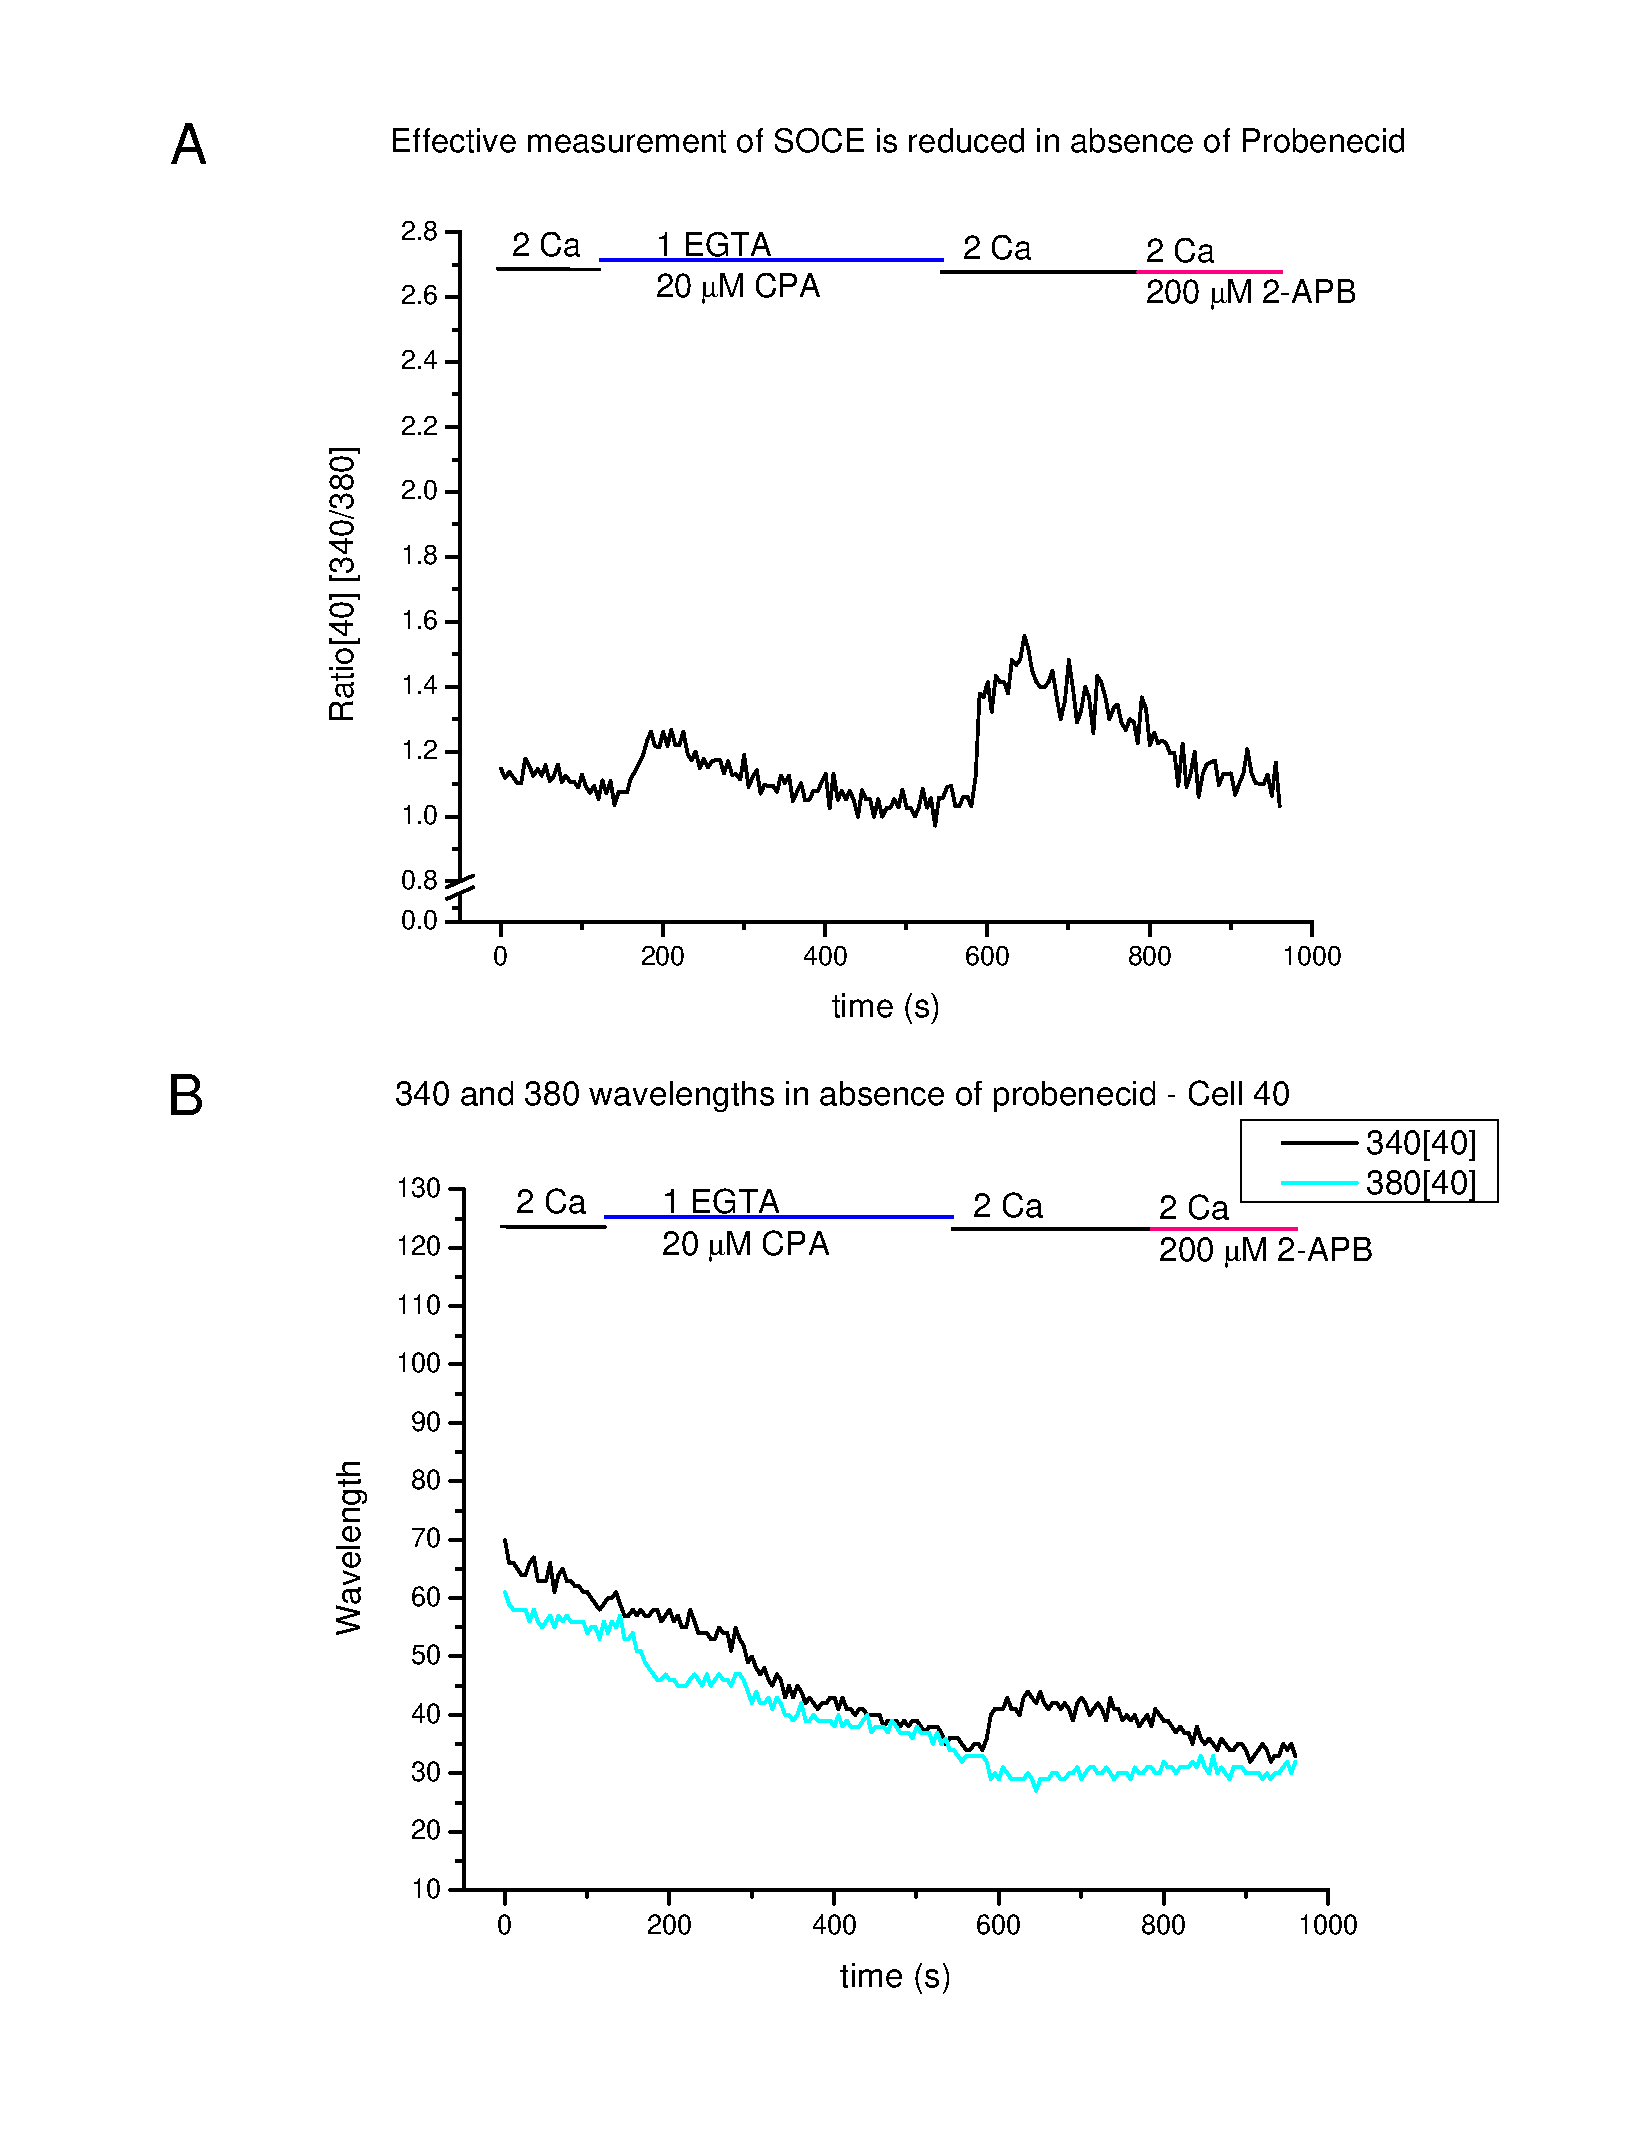
\includegraphics[scale=0.5]{Figures/s2_cell40_nopro.pdf}
\caption[Absence of probenecid gives less efficient dye loading in S2 cells]
	{{\bfseries The absence of probenecid results in less efficient dye loading in S2 cells}. ({\bfseries A}) The ratio of the 340 nm and 380 nm wavelengths of an individual cell during the course of one perfusion experiment where probenecid was omitted from the incubation solution. ({\bfseries B}) The individual 340 nm and 380 nm wavelength values, which produced the ratio seen in {\bfseries A}.}
\label{fig:s2_no_pro}
%\end{center}
\end{figure}

Figure~\ref{fig:s2_no_pro}A shows a recording from an individual S2 cell loaded without probenecid being present in the dye-loading solution (DLS).  Figure~\ref{fig:s2_no_pro}B shows the individual 340 and 380 nm wavelength values that produced the trace in A. Though the trace of the ratio hides it, we see that both wavelengths values start decreasing immediately after the start of the experiment. The decreasing values continue to the end of the experiment. The decay likely reflects leakage of Fura-2 which takes place in S2 cells if probenecid is absent in the DLS \citep{DiVirgilio1990}. The \Ca{} ratios reported after SOCE, upon reintroduction of 2 Ca are  also shown to be low here. This is most likely an artifact caused by less Fura-2 availability, thereby limiting the amount of cytoplasmic \Ca{} that can be measured.

\newpage

\begin{figure}[!ht]
%\begin{center}
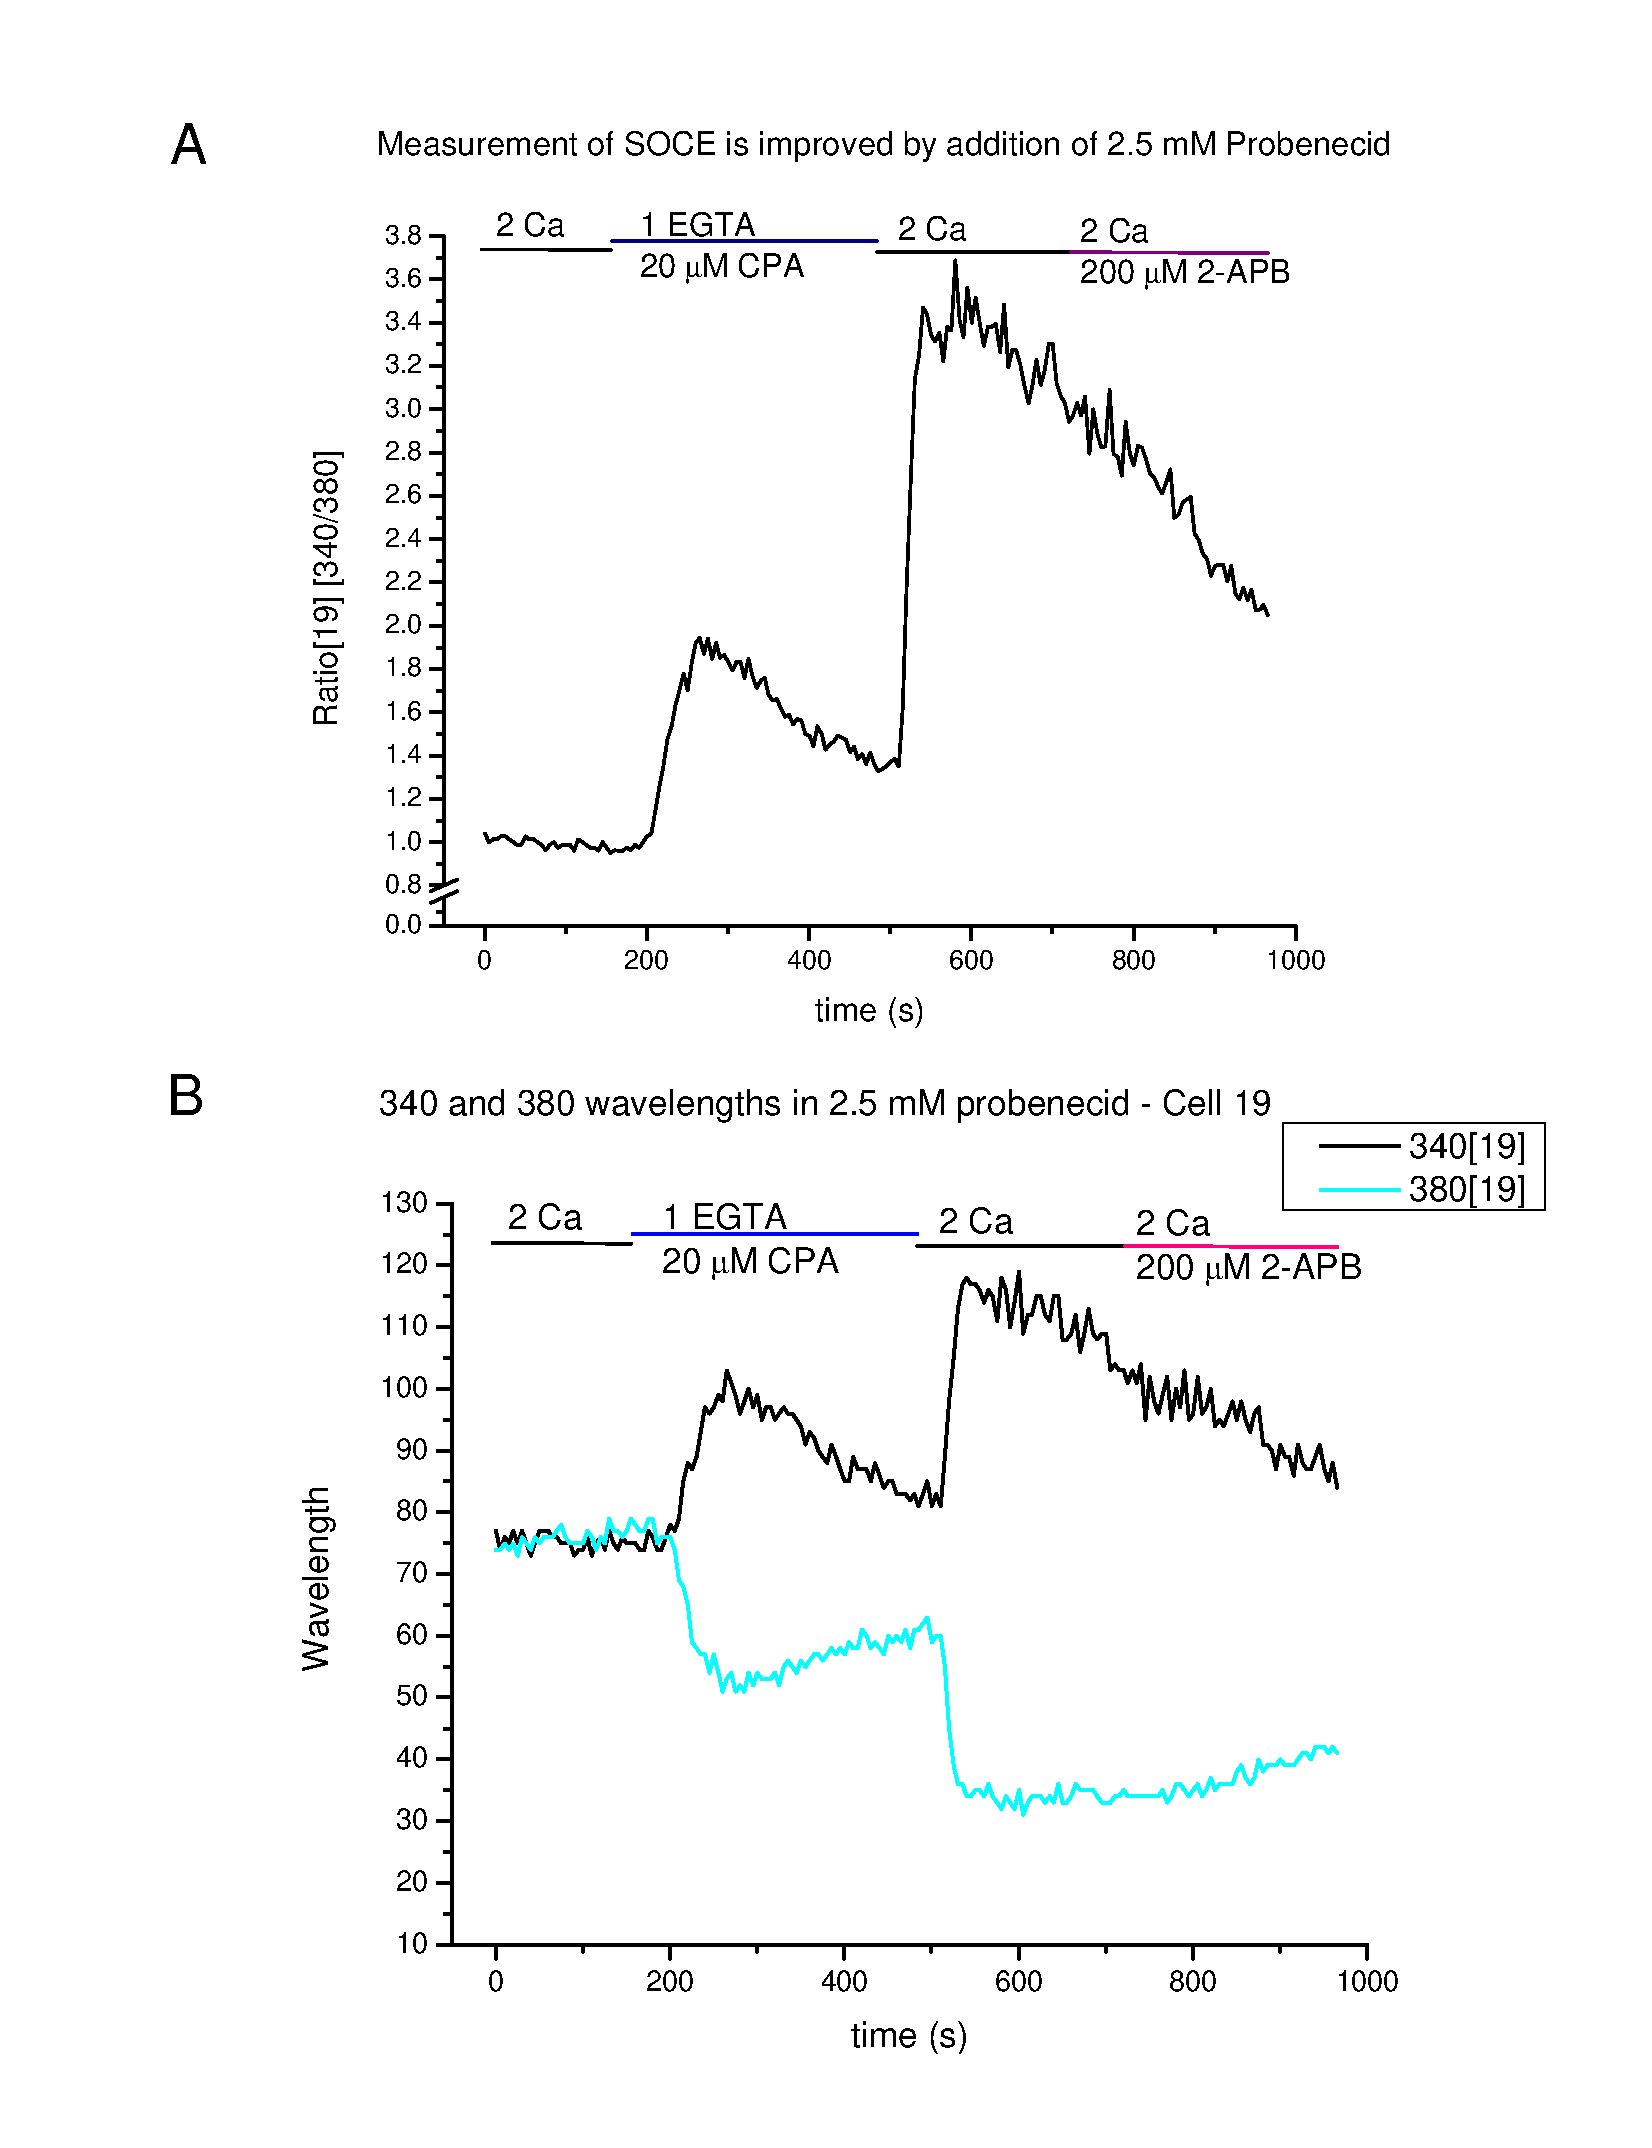
\includegraphics[scale=0.52]{Figures/s2_cell19_pro.pdf}
\caption[Probenecid improves dye loading in S2 cells]
	{{\bfseries The presence of 2.5 mM probenecid improves dye loading in S2 cells}. ({\bfseries A}) The ratio of the 340 nm and 380 nm wavelengths of an individual cell during the course of a perfusion experiment where 2.5 mM probenecid was included in the incubation solution. ({\bfseries B}) The individual 340 nm and 380 nm wavelength values, which produced the ratio seen in {\bfseries A}.}
\label{fig:s2_with_pro}
%\end{center}
\end{figure}

Figure~\ref{fig:s2_with_pro}A shows a sample recording from a cell incubated with DLS containing 2.5 mM probenecid. The ratio is robust and provides better resolution than the trace in figure~\ref{fig:s2_no_pro}. Figure~\ref{fig:s2_with_pro}B gives the individual 340 nm and 380 nm wavelengths which were used to obtain the ratio in A. We are able to clearly see the reciprocal nature of the 340 nm and 380 nm wavelength values. The steady decline of the values over the course of the experiment is no longer apparent. Probenecid has stopped or greatly slowed leakage of Fura-2 from the cytosol. As a result, we are able to record higher \Ca{} transients as more Fura-2 is available as the experiment proceeds, compared to cells loaded without probenecid. This is readily apparent in the SOCE portion of the trace. 

\newpage

\begin{figure}[!ht]
\centering
\subfloat{
	\begin{lpic}[clean]{Figures/no_pro(0.8)}
	%\includegraphics[scale=0.9]{Figures/no_pro} 
		\lbl[bl]{1,105; \bfseries A}
	\end{lpic}
}
	
\subfloat{
	\begin{lpic}[clean]{Figures/with_pro(1.3)}
	%\includegraphics[scale=1.3]{Figures/with_pro}
		\lbl[bl]{6,76; \bfseries B}
	\end{lpic}
}
\caption[Addition of Probenecid improves \Ca{} recordings]{{\bfseries Addition of Probenecid improves \Ca{} recordings}. 
({\bfseries A}) Recordings taken from a population of cells incubated in dye-loading solution that did not contain probenecid ({\bfseries B}) Recordings taken from a population of cells incubated in dye-loading solution that contained 2.5 mM probenecid.}
\label{fig:s2_pro_compare}
\end{figure}

Figure~\ref{fig:s2_pro_compare} shows a population of cells loaded without (A) and with (B) probenecid. We are able to observe a larger \Ca{} transient, due to more Fura-2 being available. Also, addition of probenecid results in more cells meeting the selection criteria for data collection. This can be attributed to Fura-2 retention in probenecid-treated S2 cells. The result is more dye being available at the start of the experiment, and as it progresses. 

Unhealthy cells, cells with damaged plasma membranes may also be omitted from the data set in a reliable, unbiased manner after probenecid treatment. Such cells would still display characteristics of untreated cells such as pronounced, persistent dye leakage.

Conditions for selecting data were formulated after examining individual 340 nm and 380 nm wavelength traces for probenecid-treated and untreated cells. Three out of six cells in A, had either 340 nm or 380 nm wavelength values below 40. This led us to use 40 as a cutoff value for data selection. For the S2 cells selected, both the 340 nm and 380 nm wavelength values stayed at or above 40 during the initial 2 Ca perfusion. This allowed for elimination of cells which were poorly loaded with Fura dye.
%leaky, even after treatment with probenecid  which, for reasons explained above, were deemed undesirable.

%\begin{figure}[htbp]
%\begin{center}
%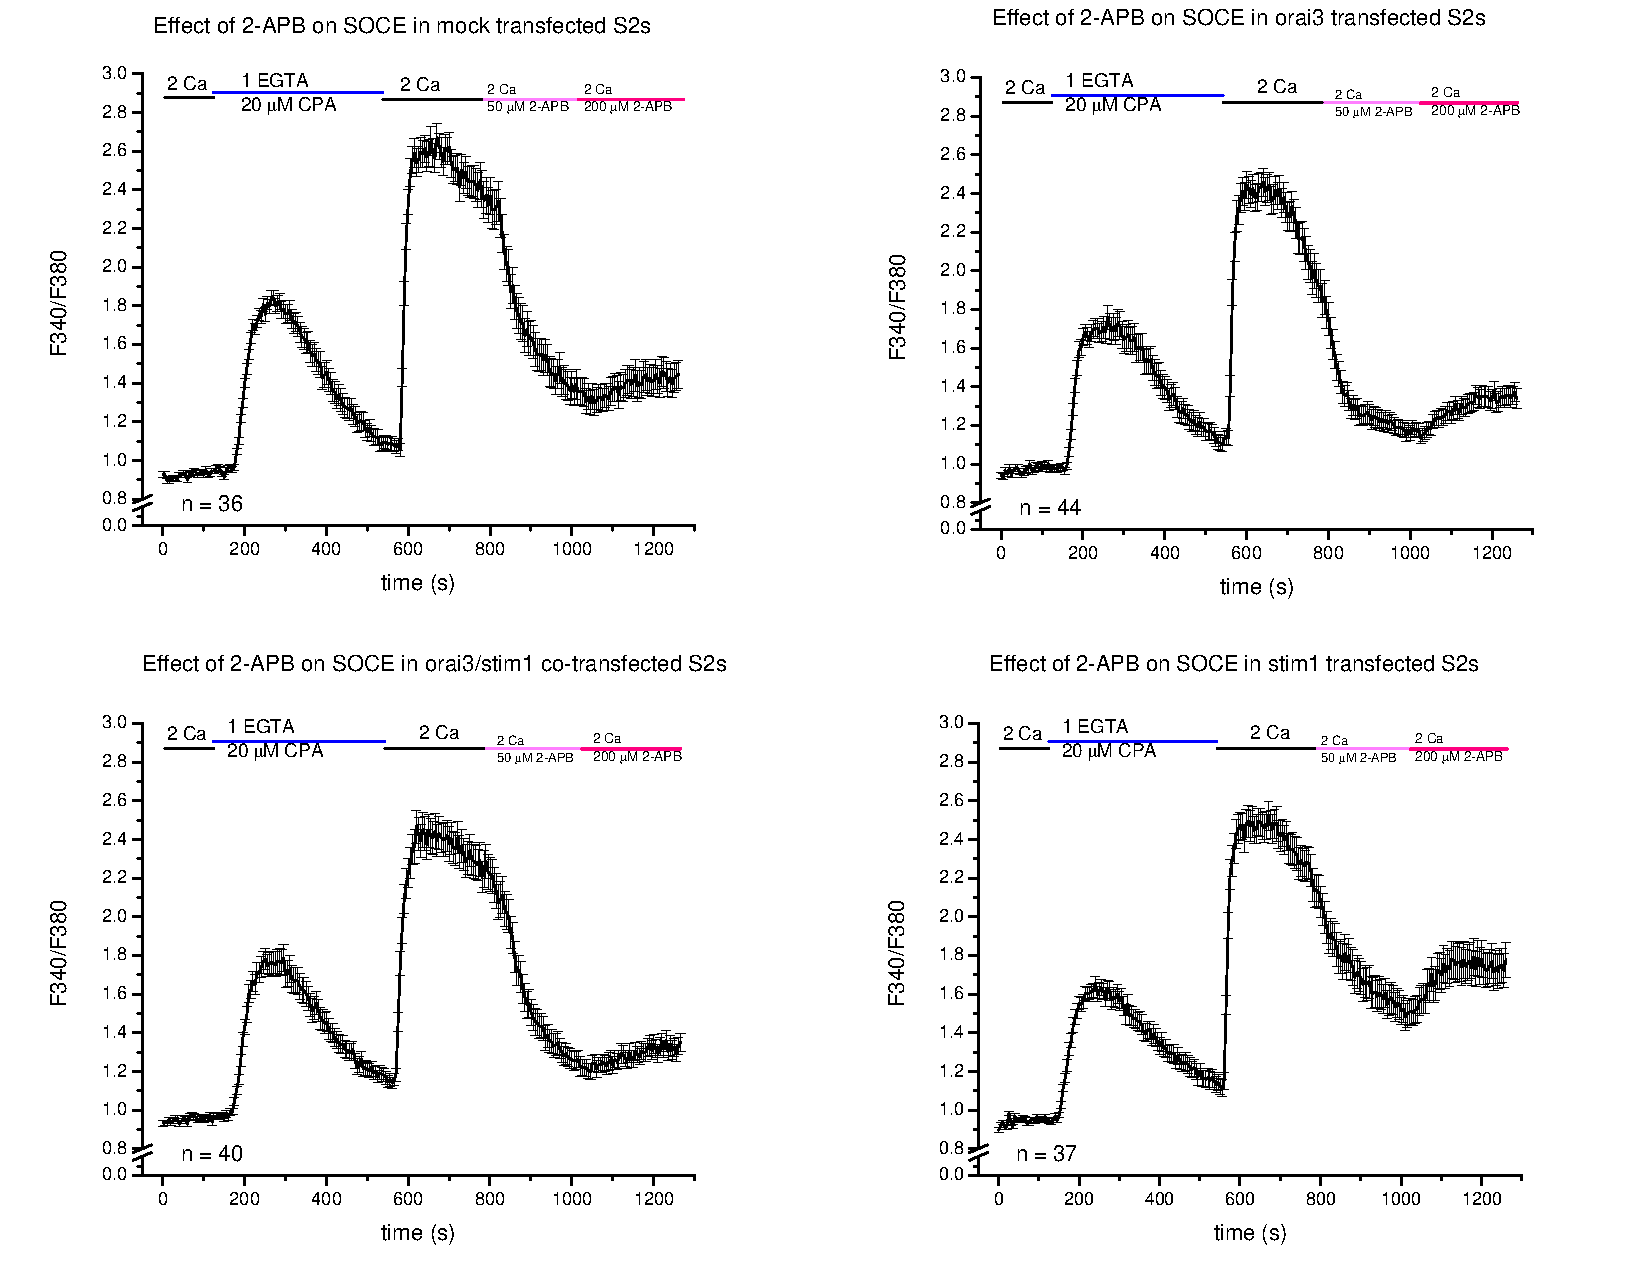
\includegraphics[clip=true, scale=0.61, trim=8mm 0 10mm 0]{Figures/s2_sample_composite}
%\caption{Ca$^{2+}$ measurements in transfected S2 cells perfused with 2-APB}
%\label{fig:s2_composite}
%\end{center}
%\end{figure}
\newpage

\begin{figure}[!ht]
	\centering
	\subfloat{
		\begin{lpic}[clean]{Figures/s2_ca_mock5_all(0.45)}
		%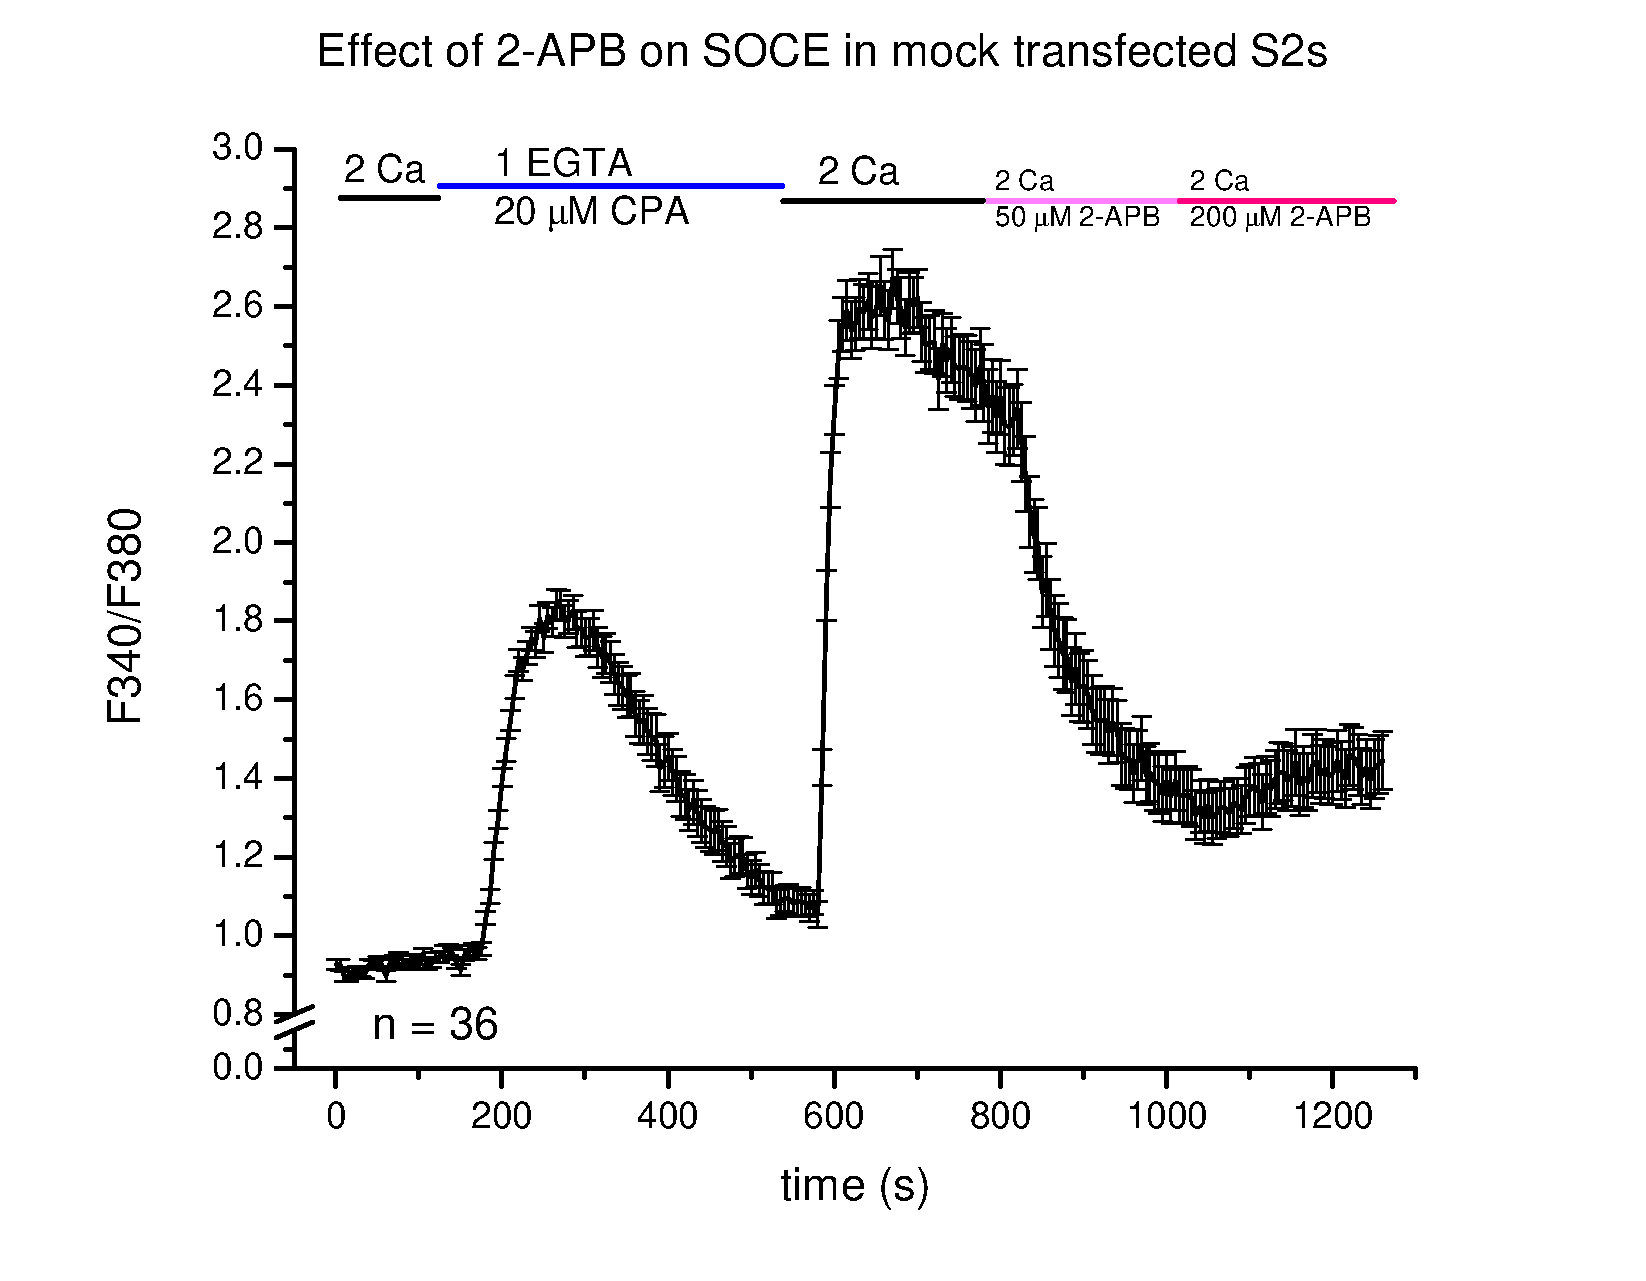
\includegraphics[scale=0.5]{Figures/s2_ca_mock5_all.pdf}
		\lbl[bl]{5,205; \bfseries A}
		\end{lpic}
	}
	
	\subfloat{
		\begin{lpic}[clean]{Figures/s2_ca_orai3_all5(0.45)}
		%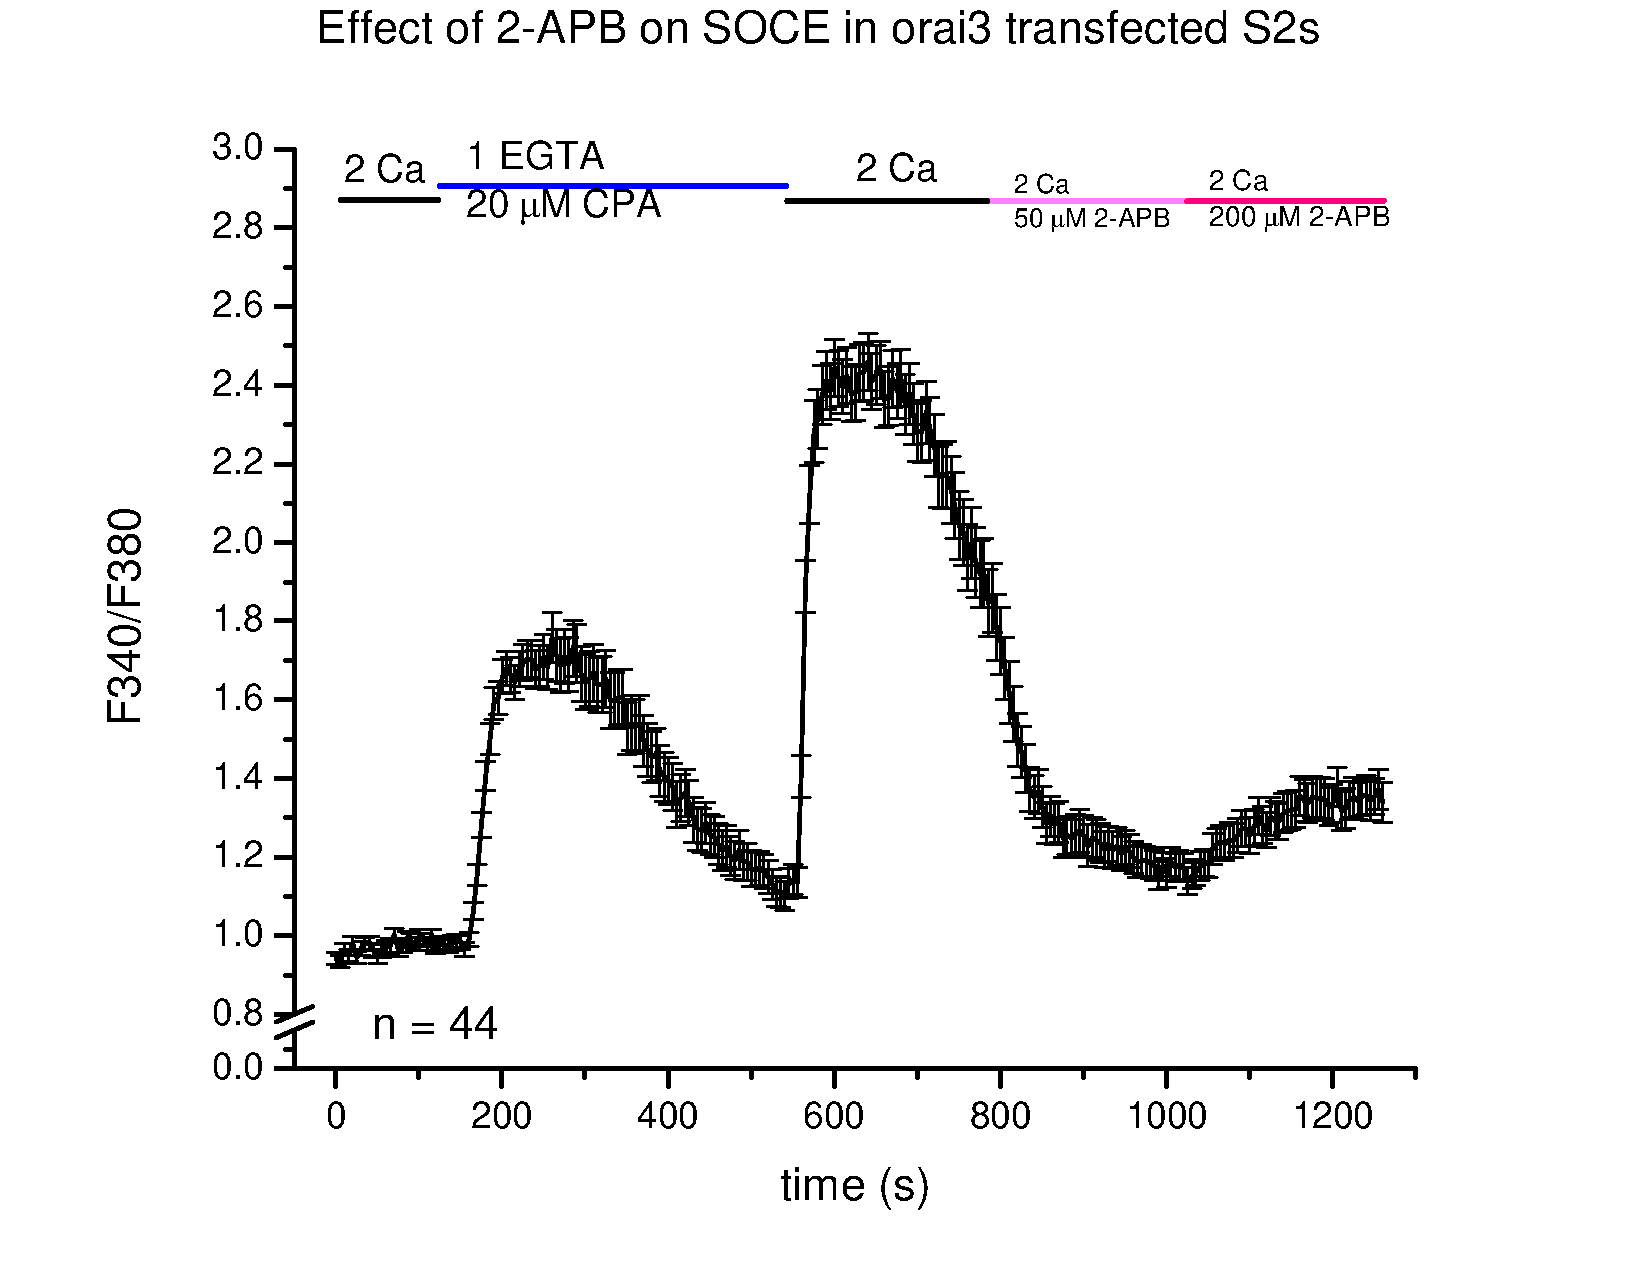
\includegraphics[scale=0.5]{Figures/s2_ca_orai3_all5.pdf}}
			\lbl[bl]{5,210; \bfseries B}
		\end{lpic}
	} 
	\caption[\Ca{} measurements in transfected S2 cells perfused with 2-APB]{{\bfseries \Ca{} measurements in transfected S2 cells perfused with 2-APB}. 	
	The lines above the trace are labeled with the solutions perfused during those times. \textbf{A}) A trace of mock-transfected S2s showing the effect of 2-APB on SOCE. \textbf{B}) A trace of Orai3-transfected S2s showing the effect of 2-APB on SOCE.}
	\label{fig:s2_composite}
\end{figure}
	
\begin{figure}[!ht]
	\centering
	\ContinuedFloat
	\subfloat{
		\begin{lpic}[clean]{Figures/s2_5_o3s1_all(0.42)}
		%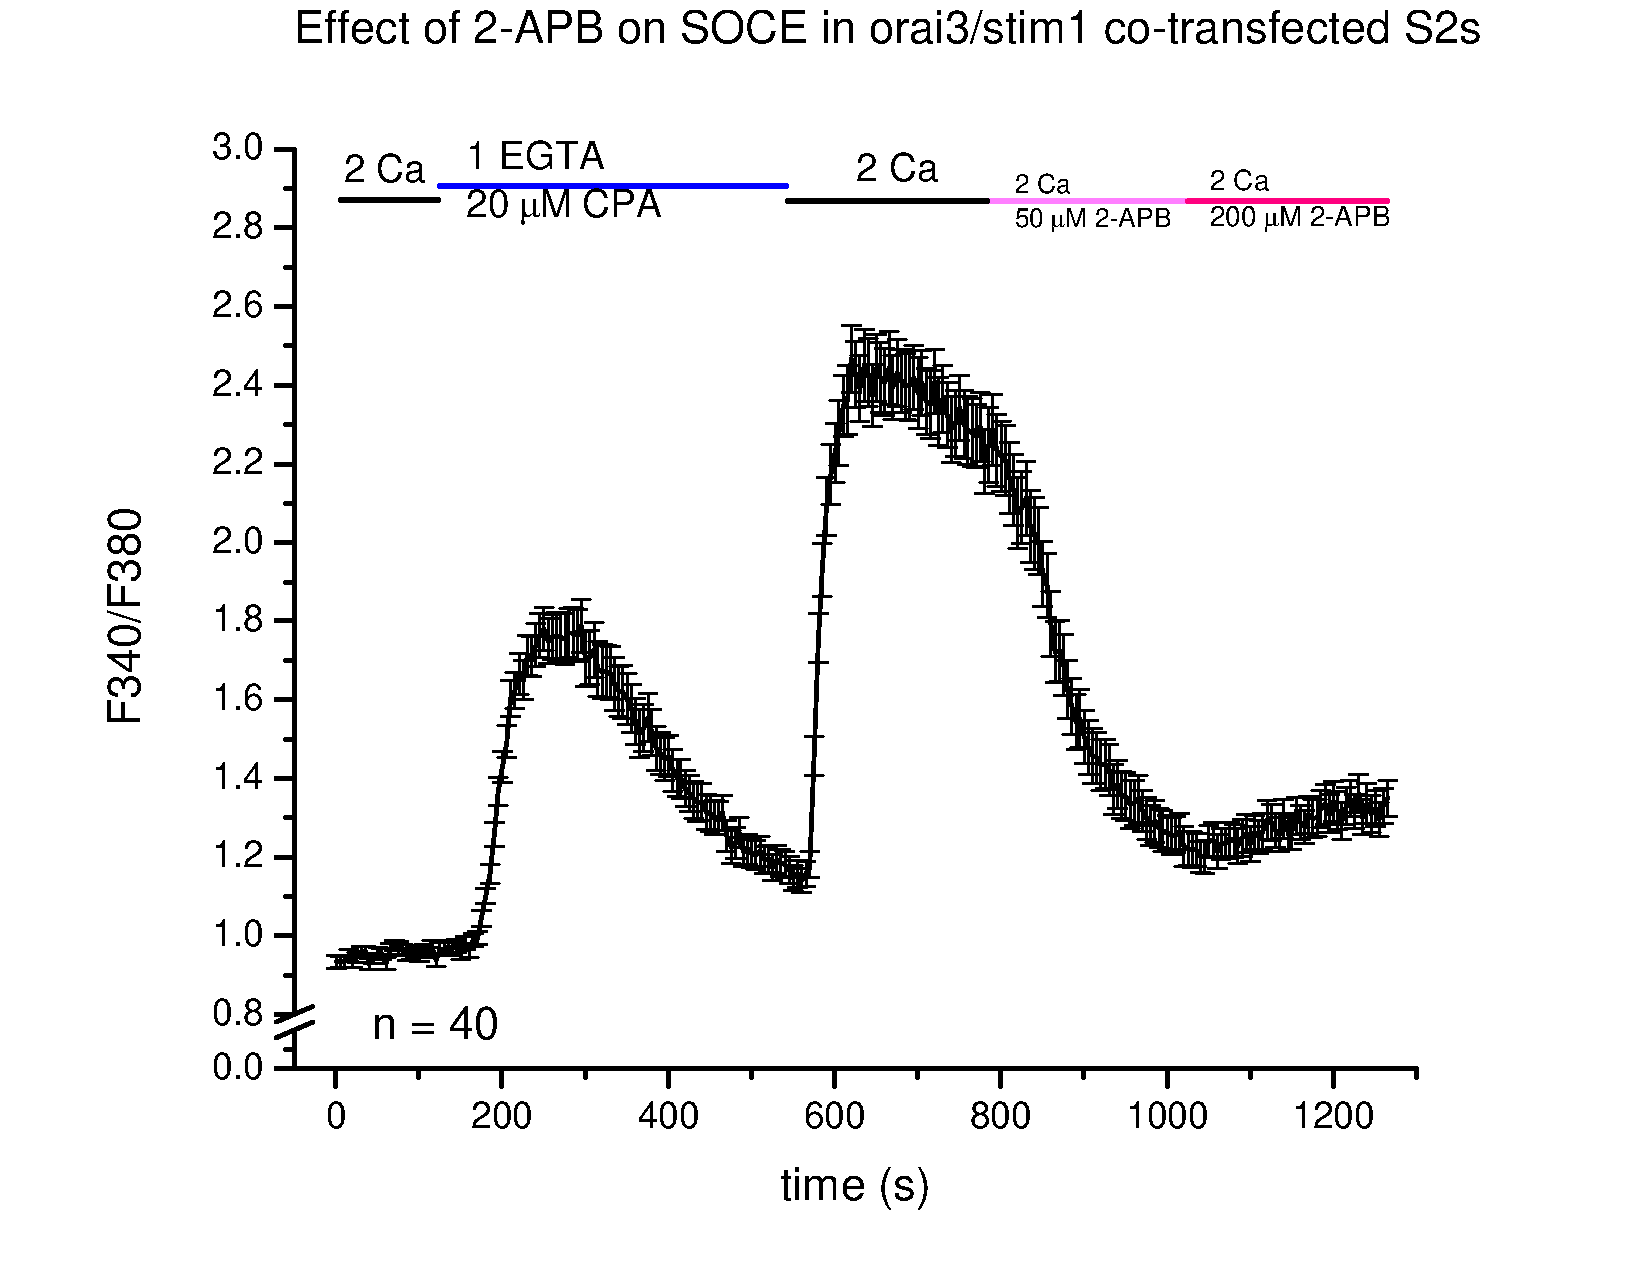
\includegraphics[scale=0.5]{Figures/s2_5_o3s1_all.pdf}
			\lbl[bl]{5,210; \bfseries C}
		\end{lpic}
	}
	
	\subfloat{
		\begin{lpic}[clean]{Figures/s2_ca_stim1_3_all(0.42)}
		%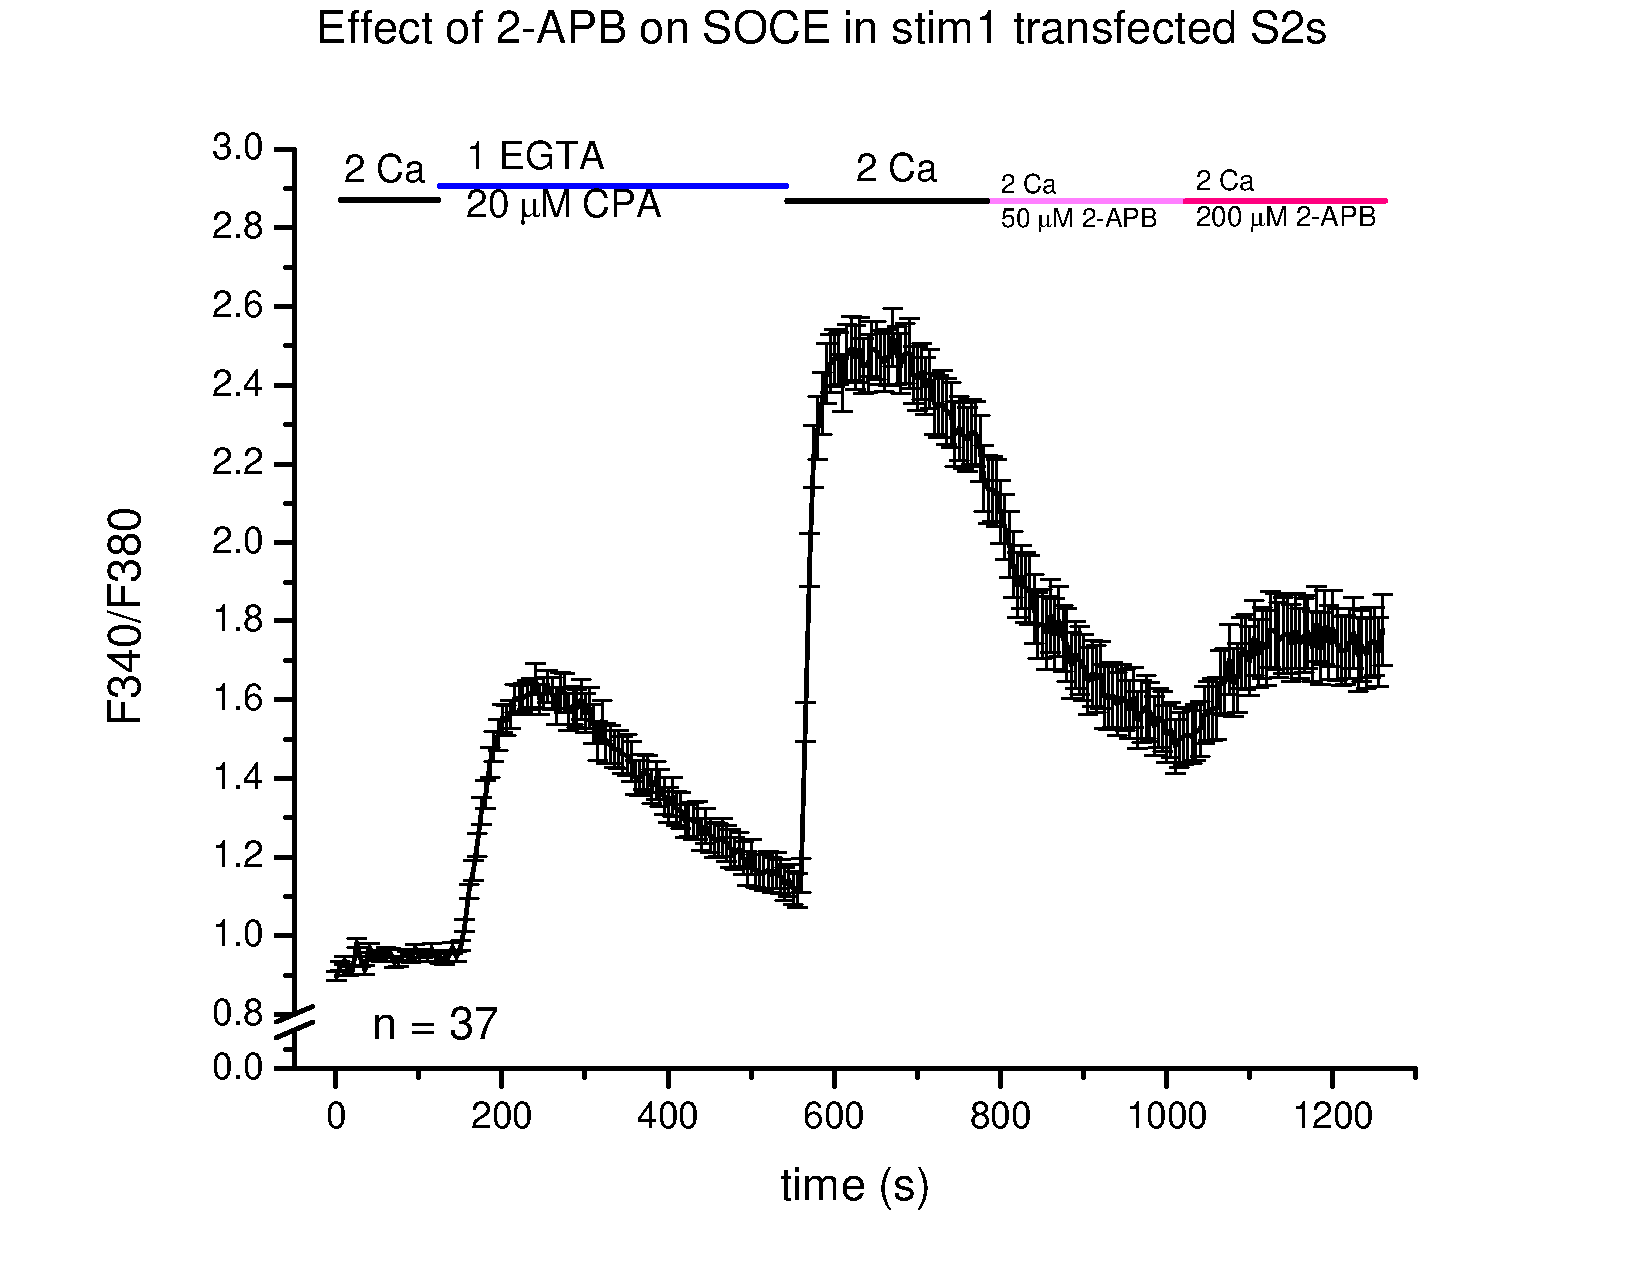
\includegraphics[scale=0.5]{Figures/s2_ca_stim1_3_all.pdf}
			\lbl[bl]{5,210; \bfseries D}
		\end{lpic}
	}
	\caption[]{{\bfseries Ca$^{2+}$ measurements in transfected S2 cells perfused with 2-APB}. 	
	The lines above the trace are labeled with the solutions perfused during those times. \textbf{C}) Sample trace of Orai3+\stim{}-transfected S2s showing the effect of 2-APB on SOCE. \textbf{D}) Sample trace of \stim{}-transfected S2s showing the effect of 2-APB on SOCE.}
	\label{fig:s2_composite}
\end{figure}


The composite in Figure~\ref{fig:s2_composite} shows representative traces for \Ca{} imaging experiments where S2 cells have been mock-transfected or transfected with Orai3, \stim{}, or Orai3+\stim.
In Figure~\ref{fig:s2_composite}A we see an average of several traces giving the result of an experiment done on mock-transfected S2s. Initially, the 2 Ca response of these mock-transfected S2s is relatively stable. Upon introduction of 20 $\mu$M CPA in 1 EGTA, we observe an increase in the F340/F380 ratio. This indicates an increase in cytosolic free \Ca, resulting from leakage of \Ca{} from the ER. This \Ca{} leak achieves a maximum and subsequently declines. The decline phase is indicative of \Ca{} being pumped out of the cell, shuttled to non-ER compartments, such as the mitochondria, or being bound by cytosolic \Ca{} chelators. Transport of \Ca{} to the ER is prevented by CPA, which blocks the SERCA pump. 

After $\sim$7 minutes of perfusion in 1 EGTA/20 $\mu$M CPA, \Ca{} is reintroduced. The mock-transfected S2s then exhibit SOCE, and a second \Ca{} transient forms at this stage. The maximal \Ca{} entry after 2 Ca reintroduction is greater than maximal \Ca{} release from the ER.  \dorai{} channels responsible for SOCE in S2 cells are able to open quickly, allowing \Ca{} into the cell shortly after switching to the 2 Ca solution.
We eventually begin to see less \Ca, which can be attributed to \dorai{} channels closing, slowing \Ca{} entry.

After 4 minutes in 2 Ca, 50 $\mu$M 2-APB is added to the perfusion solution. We see for the mock-transfected S2 cells, that the gradual decline in \Ca{} becomes sharper, shortly after addition of 2-APB. This is expected because at these concentrations 2-APB is inhibitory for \dorai{} \citep{Yeromin:2004p520}. The decline in \Ca{} continues during the 4 minutes in 50 $\mu$M 2-APB. 

After 4 minutes in 2 Ca with 50 $\mu$M 2-APB, the 2-APB concentration is increased to 200 $\mu$M 2-APB. This solution was perfused across the cells for another 4 minutes and then the experiment was stopped. During this time we observe what seems to be a slight increase. The overlap of the error bars along the trace indicate that, while there is a trend toward an increase, further analysis is required to determine its significance. In order to address the question of what happens to \Ca{}, the area under the curve was calculated for each 4-minute section after store-depletion occurred for each group of transfected cells. 

Figure~\ref{fig:s2_composite}B shows an average trace of an experiment performed on Orai3-transfected S2 cells. The initial and store-depletion phases are similar to those in the mock-transfected S2s. 2 Ca reintroduction shows a swift onset of SOCE. The expected increase in \Ca{} after addition of 50 $\mu$M 2-APB was not seen, however. Addition of 200 $\mu$M 2-APB seemed to result in a marginal increase in \Ca{} entry. The \Ca{} content of this 200 $\mu$M 2-APB phase was analyzed further and no significant change from the mock was found (see Figure~\ref{fig:s2_2apb_bar}).

%Discussion: There are a few possibilities for why this happened. The most obvious is that while Orai3 RNA production was induced with \cuso, actual protein production did not occur.Another possibility is that the transfection efficiency was consistently low with the TransIT-2020 reagent and Orai3 vector DNA. This may have resulted in poor expression of Orai3 and a paucity of Orai3 protein translation, leading to a deficiency in Orai3 channels expressed at the cellular surface. Another possibility is that, because of how closely related Orai3 and \dorai{} are, Orai3 forms heterodimers with \dorai, and adopts a phenotype primarily \dorai{} in nature.
%Testing protein expression of Orai3 proteins is possible, by isolating proteins from cells and performing a Western Blot using antibodies purchased to Orai3. 
%The generation of stable cell lines expressing Orai3 will facilitate experiments important for testing the other possibilities. \rnai{} knockdown of native \dorai{} will enable these experiments to be carried out in a background free of Orai which may be interfering with our heterologous Orai3 channel assembly. 

Since no distinct effect of 2-APB was observed in S2s transfected with Orai3 only, Orai3+\stim{} transfections were performed. We reasoned that human Orai3 may require a human \stim{} protein for coupling, rather than the background \dstim{} natively expressed in S2 cells. A trace for one of these experiments is provided in Figure~\ref{fig:s2_composite}C. 
The store-depletion and SOCE phases again seem similar to that of the mock- and Orai3-transfected cells. When treated with 50 and 200 $\mu$M 2-APB, no clear trend was visible compared to the mock- or Orai3-transfected cells.

In Figure~\ref{fig:s2_composite}D a similar experiment was performed, but on \stim{}-transfected  S2s. 
Here, the store-depletion and SOCE phases after 2 Ca reintroduction are similar to mock and other transfections. Interestingly, addition of 50 $\mu$M 2-APB in the \stim{} only transfected cells, was less effective at slowing \Ca{} entry than in the other transfections. %There seemed to be less deactivation of the \dorai{} occurring compared to the mock transfection. An alternative explanation is that another channel which allowed Ca{} into the cell was opening up due to the presence of \stim{} and 2-APB. 
When 200 $\mu$M 2-APB was added, a clear increase in cytosolic \Ca{} was observed.



\newpage

\begin{figure}[htbp]
\begin{center}
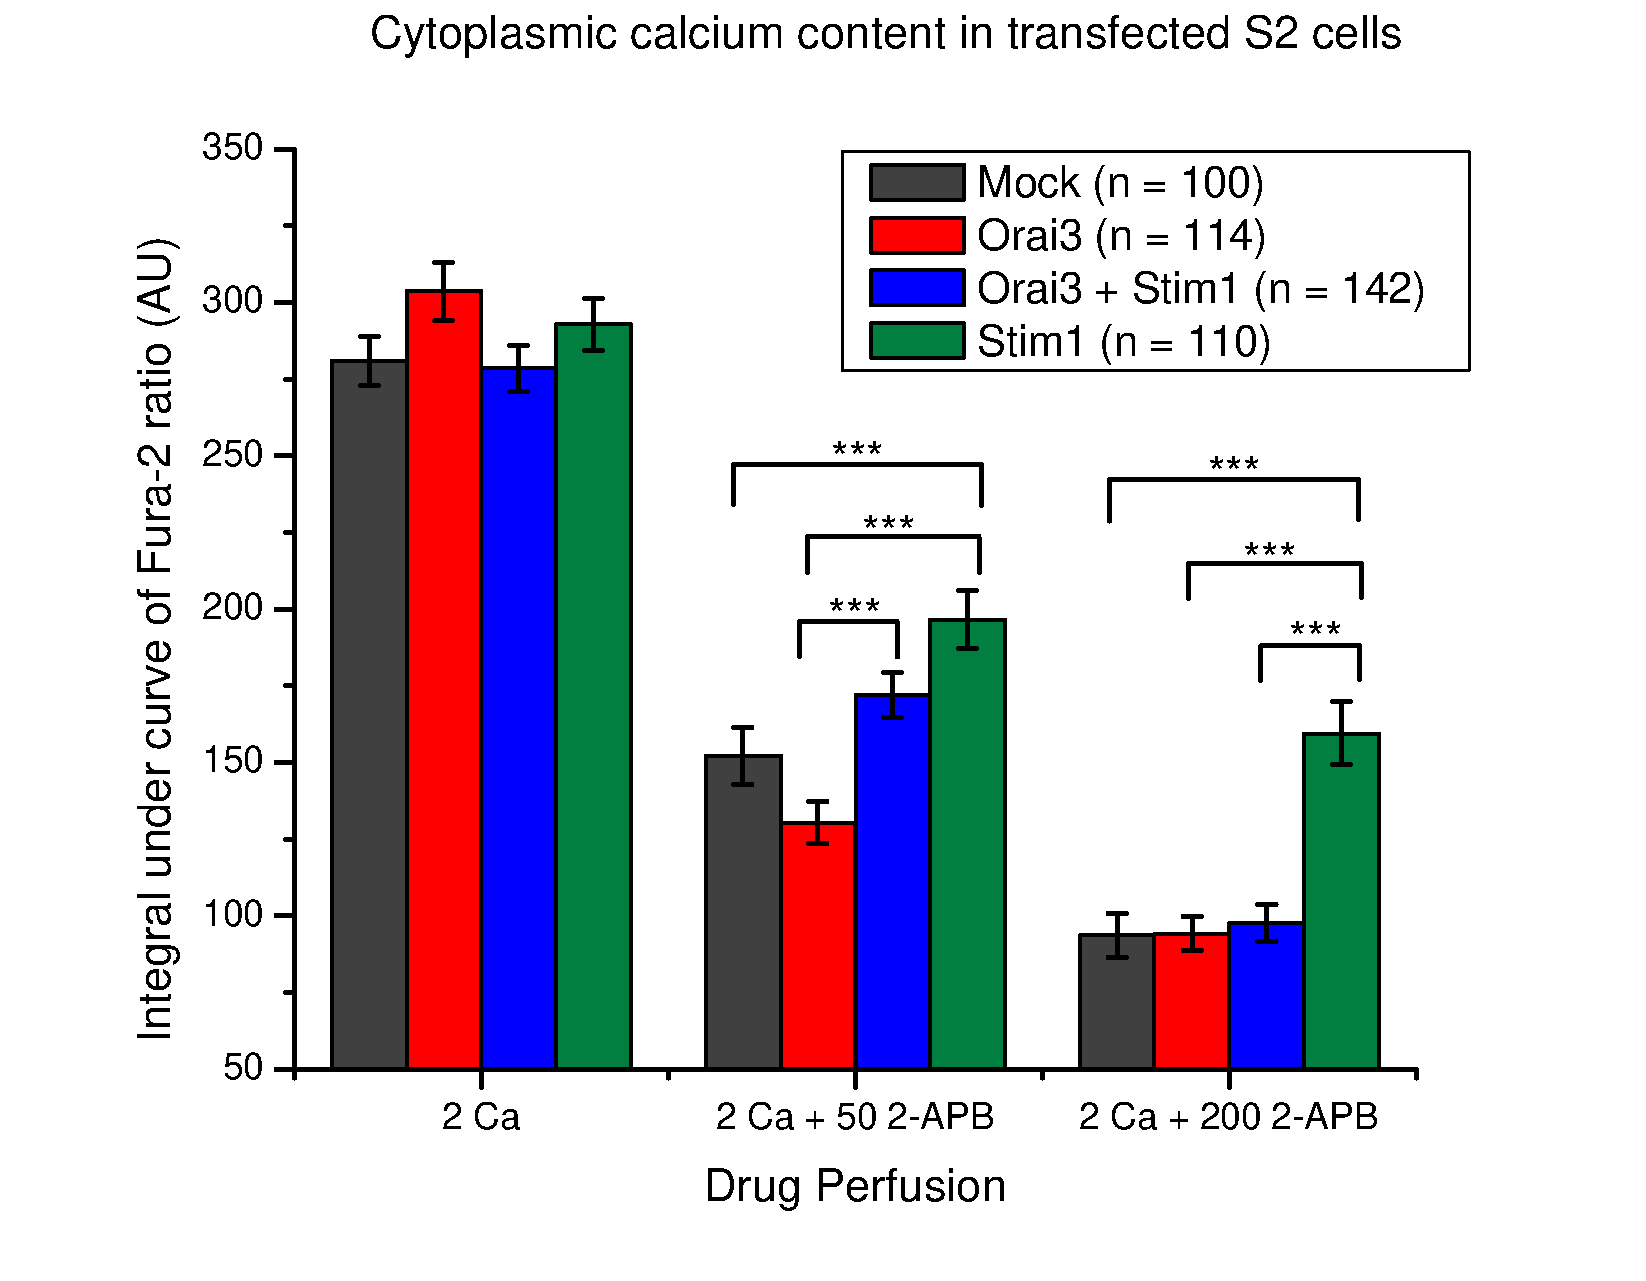
\includegraphics[clip, trim = 0 0 25mm 20mm, scale=0.6]{Figures/s2_drug_bar}
\caption[Cytoplasmic \Ca{} content in transfected S2 cells]{{\bfseries Cytoplasmic \Ca{} content in transfected S2 cells}. 
The bars represent area under the curve analysis for segments where {\bfseries 2 Ca}, {\bfseries 2 Ca + 50 $\mu$M 2-APB}, or {\bfseries 2 Ca + 200 $\mu$M 2-APB} were used to perfuse transfected S2 cells. The transfection groups are indicated in the legend. Significant differences between the transfected groups at the 0.05 significance level are indicated by ***. No significant difference was found between the 2 Ca perfusion group. Significant differences were found between the 2 Ca + 50 $\mu$M 2-APB and 2 Ca + 200 $\mu$M 2-APB perfusion groups.}
\label{fig:s2_2apb_bar}
\end{center}
\end{figure}

Figure~\ref{fig:s2_2apb_bar} displays the results of area under the curve (AUC) analysis on the three phases of treatment after store-depletion. By doing AUC analysis, the ratios generated by Fura-2 recordings were translated into cytosolic \Ca{} content of arbitrary units. The three groups in the bar graph correspond to perfusion with 2 Ca, 2 Ca + 50 $\mu$M 2-APB, and 2 Ca + 200 $\mu$M 2-APB. The perfusion time for each group was 4 minutes. A one way ANOVA was used to determine if there were significant differences in the experimental groups. If significant differences were found, Tukey's \underline{studentized} range test, was used to determine where significant differences lie between the transfection groups.  

The 2 Ca group represents an untreated period of SOCE in the transfection groups. Statistical analysis showed no significant change in cytosolic \Ca{} for this group. Functional Orai3 \Ca{} channels were expected to increase the levels of cytosolic \Ca{} during SOCE. 
%That this was not observed may be due to the \Ca{} capacity of the cell already being at maximal levels. If the S2 cell is capable of holding a finite amount of \Ca{}, and it had already reached that point, more \Ca{} channels would merely get it to that point faster, but observing further increase in \Ca{} levels would not be expected in this case.
That this was not observed may be due to the inability of Orai3 to express \emph{in the membrane}, a possibility addressed in the discussion. 

%Discussion mock:
%To determine whether the cell's cytosol was at its maximal \Ca{} carrying capacity, experiments with 2 Ca and ionomycin can be performed. After store depletion with CPA, 2 Ca can be perfusion, followed by a 2 Ca + ionomycin solution. Ionomycin is an ionophore which would raised the   \cai{} to that of the external solution. Depending on the result of perfusion with 2 Ca + ionomycin, we could say with certainty whether the maximal \Ca{} carrying capacity of the cytoplasm was reached. If for example, perfusion with ionomycin resulted in higher Ca{} levels, than was obtained without ionomycin, this would indicate that maximal levels were not obtained. 
%Discussion
%Another method for determining this would be to change the concentration of \Ca{} being used in the perfusion solution. All solutions contained 2 mM \CaCl, but decreasing the concentration to $\mu$M levels, which provide less \Ca{} for SOCE. This would result in less Ca{} being available for entry and a lower cytosolic calcium content resulting. If the \Ca{} from SOCE was still not significantly different between the transfection groups, this would allow us to conclude that the Orai3 channels were not activated solely as a function of store-depletion.


The 2 Ca + 50 2-APB experiments did show significant differences in this treatment group. 
Significant differences existed between Orai3+\stim{}-transfected cells and the Orai3 only transfected group. There were also significant differences between \stim{} only transfected cells and Orai3 only transfected cells. For both of the groups described above, the Orai3 only group showed much less cytosolic \Ca, which was unexpected. 
A significant difference was also found between mock-transfected and \stim{}-transfected cells, with the \stim{}-transfected group having higher levels of cytosolic calcium than the mock-transfected group.
The significant differences for all of the above was p $<$ 0.0001 at the 0.05 significance level. 

%Discussion:
%When only Orai3 was transfected into S2 cells and perfused with 2 Ca + 50 2-APB, a slight decrease was observed compared to mock-transfected cells, though this was not found to be significant. There were significant differences between Orai3 only and two other transfected groups: Orai3 + \stim{} and \stim{} only. That there was \emph{less} \Ca{} available in Orai3 only transfected cells, suggests that the effect of 2-APB on these  was inhibitory.
%This is supported by the finding that only \stim{}-transfected cells had significantly higher cytosolic \Ca{} than the mock-transfected cells. The difference between Orai3+\stim{} and Orai3 only transfected cells, is likely the result of the action of heterologously expressed \stim{} in this DES.


The 2 Ca + 200 2-APB showed a small but significant difference only between the \stim{}-transfected  cells and all the other groups. Again, an unexpected result which is discussed further below.  


%The \stim{} + 2-APB interaction is enhanced in higher concentrations of 2-APB. The overexpression of \stim{} in this DES may be resulting in opening of another channel by heterologous \stim{}, or alternatively slowing the deactivation of the \dorai{} responsible for the SOCE. We can see if this effect of \stim{} is specific to SOCE, by performing a similar experiment, but omitting the store depletion portion. In the absence of store-depletion, there should be no activity by \dorai{} thus any \Ca{} entry observed would likely be due to another channel. We could also test using inhibitors known to affect \dorai, such as (Ln3+?)(CITE) to determine whether the \dorai{} is being activated by \stim{} here, because \stim{} somehow changes some the characteristics of the channel. e.g. if heterologously expressed \stim{} is in the membrane, and 2-APB activates it without the need for heterologous ER \stim{} to act.

%************************

%note that perfusion of s2 cells results in near instantaneous changes in ca recordings. 
%each segment is 4 minutes long. 
%mention tukey's stat analysis
%look at probenecid - hammer that home. want to use probenecid.
%in discussion, stim1 possibilities. this vs. that.  
%Maybe Orai3 in S2s will activate in absence of store depletion.




% -eof-

% ------------------------------------------------------------------------
\chapter{Discussion}

As demonstrated in figures~\ref{fig:orai3_digests} and \ref{fig:stim1_digests} the ligation of the inserts and subsequent cloning of \oraiiiivector{} and \stimivector{} were successful. \droso{} vectors \emph{capable} of expressing mammalian Orai3 and \stim{} genes in S2 cells were created, satisfying specific aim \#1. 

Figures~\ref{fig:orai3_rtpcr} and \ref{fig:stim1_rtpcr} then showed induction of Orai3 and \stim{} \emph{gene expression} from these vectors. This demonstrated that both vector constructs actually expressed these mammalian genes in \droso{} S2 cells, satisfying specific aim \#2. Having carried out the objectives in specific aims \#1 and \#2, we moved on to address specific aim \#3: assessing the effect of 2-APB on Orai3 channels. As mentioned previously, concentrations of $\ge$ 50 $\mu$M 2-APB will activate mammalian Orai3 channels.

Initial attempts at taking \Ca{} measurements in S2 cells were thwarted by leakage of Fura-2, the \Ca{} dye being used, from these cells. As demonstrated in figures~\ref{fig:s2_no_pro}, \ref{fig:s2_with_pro} and \ref{fig:s2_pro_compare} addition of the anion transport inhibitor probenecid was crucial to recording satisfactory calcium transients. We see that omission of probenecid led to ratio measurements of SOCE transients which were lower than those recorded when probenecid was present.  Leakage of Fura-2, would have resulted in a gradual elevation of the significance of the background fluorescence. The lower ratio maxima for SOCE transients then is likely due to the low ratio caused by background fluorescence in the the cells not treated with probenecid.
%the result of less Fura-2 being present for binding to \Ca{} due to a persistent leak. 
We see that addition of probenecid reduced dye leakage by blocking the transporters responsible, and resulted in better measurements of S2 cell populations. This demonstrates that the use of probenecid for \Ca{} recordings of \droso{} S2 cells is necessary for obtaining quality data \citep{Yagodin1999}. 
 
After solving the issue of recording \Ca{} transients, assessing the effect of 2-APB on S2 cells expressing Orai3 was possible. Our hypothesis, that gene expression of mammalian Orai3 in \droso{} S2s would result in \Ca{} channels that behaved similarly to those in mammalian cells expressing Orai3 proved incorrect. As seen by the results presented in figures~\ref{fig:s2_composite} and \ref{fig:s2_2apb_bar}, Orai3 channel behavior in our  \droso{} expression system was anomalous, no increase in SOCE due to Orai3 was observed (2 Ca column, figure \ref{fig:s2_2apb_bar}). Aims \#1 and 2 were achieved, but testing of aim \#3 showed that the expression model requires further optimization. 

An unexpected and interesting result from this study was the ability of \stim{} to cause an increase in cytosolic \Ca{}. The results in figure~\ref{fig:s2_composite} for the \stim{} only transfection hint at less \emph{deactivation} of \dorai{} occurring in 50 $\mu$M 2-APB  compared to the mock transfection. Addition of 200 $\mu$M 2-APB to \stim{} only transfected S2s resulted in a clear increase in cytosolic calcium indicative of channel opening.  
One explanation is that another \Ca{} channel opened due to the combination of \stim{} and 2-APB. It may also be that 200 $\mu$M 2-APB is interacting with \stim{} leading to non-specific effects on \dorai. 
As this is only present in the \stim{} transfected cells, and since the amount of \stim{} DNA used in \stim{} and Orai3+\stim{} transfections was the same (2 $\mu$g) this suggests an effector+2-APB interaction in the absence of Orai3. 

%The presence of mammalian \stim{} with 200 µM 2-APB, while not able to increase SOCE, slows the inactivation of \dorai. This results in a significant increase of intracellular calcium, when compared to the mock and other transfections. Support for theory of alteration of pore selectivity? If the slowing of inactivation of \dorai{} currents was due to an increase in the 2-APB which somehow affected the SERCA pump, a drug whose effects are not reversible (personal communication, Dr. J. Ashot Kozak), then we would expect to see similar results in all the other transfections, due to the effects of the hypothetical CPA washout. 
%Figure~\ref{fig:s2_2apb_bar}

%Discussion mock:
%To determine whether the cell's cytosol was at its maximal \Ca{} carrying capacity, experiments with 2 Ca and ionomycin can be performed. After store depletion with CPA, 2 Ca can be perfusion, followed by a 2 Ca + ionomycin solution. Ionomycin is an ionophore which would raised the   \cai{} to that of the external solution. Depending on the result of perfusion with 2 Ca + ionomycin, we could say with certainty whether the maximal \Ca{} carrying capacity of the cytoplasm was reached. If for example, perfusion with ionomycin resulted in higher Ca{} levels, than was obtained without ionomycin, this would indicate that maximal levels were not obtained. 

%Another method for determining this would be to change the concentration of \Ca{} being used in the perfusion solution. All solutions contained 2 mM \CaCl, but decreasing the concentration to $\mu$M levels, which provide less \Ca{} for SOCE. This would result in less Ca{} being available for entry and a lower cytosolic calcium content resulting. If the \Ca{} from SOCE was still not significantly different between the transfection groups, this would allow us to conclude that the Orai3 channels were not activated solely as a function of store-depletion.



%By using directional cloning techniques we were able to quickly generate our desired constructs. Restriction digest analysis was used to determine whether Orai3 and \stim{} were inserted into \puchygmt{} in the intended orientation. The size of the \sali{}+\xbai{} digested vector was taken to be quite close to 7000 bp, as no clear band was visible at 100 bp or higher. Given that these sites were in the multiple cloning region, and given the closeness of the sites on the provided map, it is likely that only a few base pairs separated the sites. The original vector map can be seen in the supplemental data.

%In figure~\ref{fig:orai3_digests} \bamhi{} and \xhoi{} were used to digest \oraiiiivector{} and determine the insert size. In the absence of an insert, a sole $\sim$7000 bp would be observable on the gel. The presence of the $\sim$6957 bp and 931 bp bands indicated that Orai3 insertion was successful.

%\bamhi{} and \xhoi{} were selected because \sali{} and \xbai{} digestion did not produce the expected bands. Further analysis uncovered that this was due to the \xbai{} site being blocked as a result of a dam methylation. The {\tt TGA} stop codon of Orai3 combined with the {\tt TCTAGA} \xbai{} restriction site, introduced a {\tt GATC} dam methylation site. The result was a linearized \oraiiiivector{} after \sali+\xbai{} double digestion, because \xbai{} is blocked by dam methylation.
%See supplemental figure.\todo{create supplemental figure for this}are present in \puchygmt{}. 

%The use of \kpni{}, whose site is specific to Orai3 and \xhoi, specific to the vector allowed us to determine whether Orai3 inserted properly. Successful insertion in the 5\'{} to 3\'{} direction, would yield the 796 bp band observed in lane 3 of figure~\ref{fig:orai3_digests}. 
%After restriction digest analysis, clones which displayed the expected bands were sent for sequence verification. 
%Sequence analysis on \oraiiiivector{} found no mutations in the Orai3 sequence. This experiment and the subsequent sequence analysis were important in providing confirmation that the \oraiiiivector{} construct was successfully generated. %The sequence of \oraiiiivector, can be seen in the supplemental data.


%With our \stimivector{} construct, there were no issues with dam methylation, and so \xbai{} could be used. Lane 4 shows the 2066 bp and $\sim$6994 bp bands we expect from \sali+\xbai{} digestion, along with a linearized $\sim$9060 bp product. The result of \stui+\xhoi{} and \bamhi+\stui{}  digestions in lanes 1 and 2 respectively,  confirm insertion of \stim in the correct direction. Together, these restriction digests confirm that the \stimivector{} was also successfully created, and in the proper direction. Following restriction digest analysis, \stimivector{} clones which displayed the expected bands were also sent for sequence verification. Sequence analysis on \stimivector{} DNA confirmed the sequence and direction of \stim{} insertion as well.  



There are several possibilities for why Orai3, either alone or with \stim{}, did not display the expected \Ca{} increase after addition of 50 or 200 $\mu$M 2-APB. The most obvious is that while Orai3 RNA production was induced with \cuso, actual protein production did not occur by the time of the experiments. Another possibility is that the transfection efficiency was consistently low with the transfection reagent and \oraiiiivector{} DNA. This may have resulted in poor expression of Orai3 and a paucity of Orai3 protein translation, leading to a deficiency in Orai3 channels expressed at the cellular surface.
Another possibility is that, because of how closely related Orai3 and \dorai{} are -- a BLAST comparison shows a 64\% nucleotide sequence similarity -- Orai3 forms heteromers with \dorai, and adopts a phenotype primarily \dorai{} dominated in nature.  

Given that \stim{} expression results in an unexpected phenotype, it is unlikely that Orai3, the smaller protein which was made in a similar manner, does not express. It is more likely that interactions with the closely related \dorai{} result in heteromeric channels, and it is the output from those channels that we are investigating.

Transfection of Orai3 with \stim{} did lead to a significant increase in cytosolic \Ca{} compared to Orai3 only transfected cells (see figure~\ref{fig:s2_2apb_bar}). This suggests that \dstim{} is not sufficient for Orai3 function.
 
Future work on this project will involve testing the possibilities presented above, for why Orai3 activation did not occur after 2-APB treatment. The generation of stable cell lines using the hygromycin B resistance conferred by \puchygmt{}  is underway. While creating clonal populations of stably selected S2 cells is possible, reports indicate that the additional effort does not seem worthwhile \cite{Schetz2004}. Expression levels for high-expressing clones seem similar to those from a polyclonal population \cite{Schetz2004}.
Stable lines expressing  Orai3 and \stim{} together will facilitate experiments needed to test these possibilities. 

Protein expression of Orai3 can be tested by isolating proteins from transfected cells and performing Western Blot analysis using antibodies to Orai3. Testing for interference from native \dorai{} by performing \rnai{} knockdown will address the issue of \dorai{} influencing the Orai3 channel phenotypes. Beyond the potential issue of \dorai{} affecting Orai3 function and/or expression, \rnai{} knockdown of \dorai{} allows study of Orai3 channels in isolation on a \dorai{}-free background. This will be useful for defining Orai3 channel function, as opposed to general SOCE, to which Orai3 may contribute.

\section{Conclusion}
The creation of an expression system for mammalian Orai \Ca{} channels to be used for drug discovery purposes was begun in this study. The proteins selected to probe the feasibility of using such a system were the mammalian Orai3 \Ca{} channel, and mammalian \Ca{} sensor \stim. Constructs for expression in S2 cells were created and were able to successfully express genes from both Orai3, and \stim. Our \droso{} system was not able to reproduce the function of the Orai3 channel in the presence of the known effector 2-APB, highlighting the need for further refinement, before use in future drug studies. Provided that the issues with channel expression are solved, the system has the potential to be a very useful tool, for study of not just Orai3, but the entire Orai family. 

The system is effective in inducing RNA expression of Orai3 and \stim{}, however, and is currently being used to generate stable cell lines to further this study. Given the importance of SOCE to the adaptive immune response and related disease states, this initial work and future studies based upon it, have the potential to be important vehicles for contributing to the body of knowledge in the field of \Ca{} metabolism. Studies of diseases resulting from disrupted \Ca{} homeostasis, including forms of cancer and autoimmune diseases, may also benefit from the creation of this expression system.




%\newpage 

%\section{Discussion \& Future Work}
%It is possible that the endogenous \dorai{} and \dstim{} proteins will, on the basis of their similarity with the human orthologs, have some contribution to the \Ca{} measurements obtained. \\droso{} are very amenable to RNA interference (RNAi), which can be used to knock down specific genes, based on their sequence. Future work will be to create stable cell lines,  expressing our genes of interest. The vectors used, were designed with this goal in mind, and only Hygromycin B selection of S2 cells transfected with our construct remains. 
%Furthermore, by knocking down \dorai{} and \dstim{} using RNAi, and repeating the experiments, the contribution of the endogenous genes can be determined.

%More work is necessary to make this system useable for the purpose of drug discovery, but the foundation of this work has already been laid. Creation of stable cell lines expressing our genes of interest is currently being undertaken. These stably expressed \stim{} and Orai3 lines will allow us to answer questions on protein expression of the channel. Due to the unexpected result we get from \stim{} expression with 200 $\mu$ 2-APB, it is very unlikely that \stim{} is not being expressed. 
%The stable cell line will allow us to study the novel behavior of \stim{} in this model system. important questions such as, the channel heterologous \stim{} seems to be affecting, will be answered more easily due to the creation of this cell line. 
%************ Given that \stim{} expresses, it seems unlikely that Orai3, which was made in a similar manner is not expressing. 
%************ More likely it is interacting with \dorai{} and the result of these heteromeric channels are what we are looking at.

%See supplemental figure. GFP only, Stim1 + GFP transient transfection, STIM1 + GFP after 1 month of selection.
%See supplemental figure. No 2-APB in untransfected cells.  

%%%%%%%%%%%%%% NOTICE MEEEE %%%%%%%%%%%%%%%%%
%See Goto2010 for example of ORAI3 activation dependent on STIM. Precedent exists. 

 
% ------------------------------------------------------------------------
%\include{Chapters/conclusion}
% ------------------------------------------------------------------------
%\include{Chapter/supplement}
% ------------------------------------------------------------------------
%\include{chapter7}
% ------------------------------------------------------------------------
%\include{chapter8}
% ------------------------------------------------------------------------
\renewcommand\baselinestretch{1.5}
\addcontentsline{toc}{chapter}{Bibliography}
%\bibliographystyle{acmtrans}
%\citestyle{nature}
%\bibpunct{(}{)}{,}{n}{}{;}
%\bibliographystyle{plainnat}% You should chose one for your major. Look for bst styles on ctan, or use makebst.sty. This formats the bibliography
%\bibliographystyle{asmems4}
\bibliography{library}
 
 
%\appendix

%\chapter{First appendix chapter}
%Oh, there can be an appendix. 
%\include{appendixA}
%\include{appendixB}
%\include{appendixC}
%\include{appendixD}

%-----------------------------------------------------------------------
\end{document}
%-----------------------------------------------------------------------
